\documentclass[a4paper, 12pt, oneside]{book}

\usepackage[utf8]{inputenc}
\usepackage{lmodern}
\usepackage{layout}
\usepackage{emptypage}
\usepackage{fancyhdr}
\usepackage{subfigure} % subfiguras
\usepackage{caption}
\usepackage{mathtools}
\usepackage[a4paper,top=3cm, bottom=3cm, inner=2.5cm, outer=2.5cm]{geometry}
\usepackage{listings}
\usepackage[spanish]{babel}
\usepackage{float}
\usepackage{multirow}
\usepackage{rotating} 
\usepackage{color}
\usepackage{colortbl}
\usepackage[table]{xcolor}
\usepackage[spanish]{babel}
\usepackage{tikz}
\usetikzlibrary{shapes.geometric, arrows}
\usepackage[bottom]{footmisc}
\usepackage{amssymb}
\usepackage{booktabs,array}
\usepackage[hyphens]{url}
\usepackage[hidelinks]{hyperref}
\hypersetup{breaklinks=true}
\urlstyle{same}

\definecolor{greenyellow}{RGB}{173,255,47}
\definecolor{darkgreen}{RGB}{34,139,34}
\definecolor{myorange}{RGB}{255,153,51}

\PassOptionsToPackage{hyphens}{url}\usepackage{hyperref}

\tikzset{
  treenode/.style = {shape=rectangle, rounded corners,
                     draw, anchor=center,
                     text width=3cm, align=center,
                     top color=white, bottom color=blue!20,
                     inner sep=1ex},
  treenodelong/.style = {shape=rectangle, rounded corners,
                     draw, anchor=center, minimum height = 1cm,
                     text width=6cm, align=center,
                     top color=white, bottom color=blue!20,
                     inner sep=1ex},
  decision/.style = {treenode, diamond,  aspect=2, inner sep=0pt,
                     text centered, draw=black},
  arrow/.style = {thick,->,>=stealth}
}

\usepackage{dirtree}
\usepackage{mdwlist}


\usepackage[acronym, nonumberlist]{glossaries}
\makeglossaries
\newacronym{urm}{MRU}{Movimiento Rectilíneo Uniforme}
\newacronym{dof}{DOF}{Grado de libertad}
\newacronym{dofs}{DOF}{Grados de libertad}
\newacronym{mlp}{MLP}{\textit{Multilayer Perceptron}}
\newacronym{lstm}{LSTM}{\textit{Long Short-Term Memory}}

\makeatletter
\renewcommand{\@makeschapterhead}[1]{%
%  \vspace*{50\p@}%
  \vspace*{0\p@}%
  {\parindent \z@ \raggedright
    \normalfont
    \interlinepenalty\@M
    \Huge \bfseries  #1\par \nobreak
%    \vskip 40\p@
    \vskip 15\p@
  }}
\makeatother

\renewcommand{\baselinestretch}{1.4}
\setlength{\headheight}{16pt} 
\captionsetup{justification=justified}
\pretolerance=1000

\chead[]{}
\rhead[]{}
\renewcommand{\headrulewidth}{0.5pt}

\pagestyle{empty}

\title{Predicción de fotogramas}
\author{Nuria Oyaga de Frutos}

\lstset{
	float=hbp,
	basicstyle=\ttfamily\small,
	columns=flexible,
	tabsize=4,
	frame=single,
	extendedchars=true,
	showspaces=false,
	showstringspaces=false,
	numbers=none,
	numberstyle=\tiny,
	breaklines=false,
	breakautoindent=true,
	captionpos=b
}
\setcounter{tocdepth}{4}
\setcounter{secnumdepth}{4}

\definecolor{lightgray}{gray}{0.9}

\begin{document}
%%%%%%%%%%%%%%% Portada %%%%%%%%%%%%%%%%%%%%
\begin{titlepage}
	\begin{center}
		\begin{center}
			
\includegraphics[width=0.4\linewidth]{figures/logo}
		\end{center}
		\vspace{7.5mm}
		
		\fontsize{15.5}{14}\selectfont ESCUELA TÉCNICA SUPERIOR DE INGENIERÍA INFORMÁTICA
		\vspace{13mm}
		
		\fontsize{14}{14}\selectfont MÁSTER UNIVERSITARIO EN VISIÓN ARTIFICIAL 
		
		\vspace{70pt}
		
		\fontfamily{lmss}\fontsize{15.7}{14}\selectfont \textbf{TRABAJO FIN DE MÁSTER} 
		
		\vspace{20mm}
		\begin{huge}
			Predicción de fotogramas \vspace{0.4cm} \\ con Redes Neuronales
		\end{huge}
		
		\vspace{35mm}
		
		\begin{large}
			Autor: Nuria Oyaga de Frutos
			
			Tutor: José María Cañas Plaza
			
			Cotutor: Inmaculada Mora Jiménez
			
			\vspace{20mm}
		\end{large}
		\begin{normalsize}
			Curso académico 2019/2020	
		\end{normalsize}
		\vspace{10mm}
		
	\end{center}
	
\end{titlepage}

\pagebreak
\thispagestyle{empty}
\vspace*{12cm}

\begin{flushright}


\includegraphics[height=1.0cm]{figures/CC-BY-SA.png}

\vspace*{0.5cm}

\copyright 2020 Nuria Oyaga de Frutos

\vspace*{0.3cm}

Esta obra está distribuida bajo la licencia de 

``Reconocimiento-CompartirIgual 4.0 Internacional (CC BY-SA 4.0)''

de Creative Commons.

\vspace{0.2cm}

Para ver una copia de esta licencia, visite

http://creativecommons.org/licenses/by-sa/4.0/ o envíe

una carta a Creative Commons, 171 Second Street, Suite 300,

San Francisco, California 94105, USA.

\end{flushright}

\pagenumbering{Roman}

%%%%%%%%%%%%%%% Agradecimientos %%%%%%%%%%%%
{
	\vspace*{1cm}
	\begin{flushright}
		\textit{"The way to get started is to quit talking and begin doing"}\\
		\vspace{10pt}
		-Walt Disney-
	\end{flushright}
	
	\vspace*{14cm}
	\begin{flushright}
		\textit{A mi rosa mas bonita,\\
		la más bella del rosal,\\
		gracias por enseñarme,\\
		lo que es vivir y luchar.}
	\end{flushright}
}

\chapter*{Agradecimientos}

En primer lugar quiero dar las gracias...\\

\begin{flushright}
	\emph{¡Muchísimas gracias a todos!}
\end{flushright}


%%%%%%%%%%%%%%% Resumen %%%%%%%%%%%%%%%%%%%%
\chapter*{Resumen}

En los últimos años, la investigación en Visión Artificial para que las máquinas puedan percibir el mundo físico que les rodea, al igual que hace el ser humano mediante la vista, ha experimentado un gran desarrollo. En este aspecto, el uso de arquitecturas neuronales profundas cuyo aprendizaje está dirigido por conjuntos de datos representativos de la tarea a abordar, ha permitido mejorar las prestaciones de los algoritmos tradicionales. De las tres tareas que pueden realizar las estructuras neuronales, detección, clasificación y predicción, la predicción visual es la menos común. Además, dicha tarea tiene un largo recorrido en su investigación y una gran utilidad. Es por ello que este trabajo fin de máster aborda la tarea de predicción haciendo uso de secuencias de imágenes con un elemento móvil.\\

Se ha realizado un estudio sobre cómo distintas estructuras neuronales, de naturaleza recurrente y no recurrente, pueden utilizarse para realizar la predicción de fotogramas en una secuencia de vídeo, donde las correlaciones espacio-temporales entre imágenes son importantes. Para ello, se ha creado una serie de secuencias sintéticas formadas por fotogramas en los que un único píxel activo se desplaza siguiendo una determinada dinámica temporal: lineal, parabólica o sinusoidal. Así mismo, se han considerado los fotogramas en dos formatos distintos, uno modelado, que reduce toda la imagen a las posiciones (\textit{x}, \textit{y}) del píxel activo, y otro crudo, que representa la imagen como una matriz 2D de píxeles. Para obtener las secuencias sintéticas,  se ha desarrollado un generador que permite crear ejemplos adaptados a un tipo de estudio concreto.\\

Con la realización de esta investigación se ha comprobado que, bajo determinadas hipótesis, es posible predecir satisfactoriamente la posición del objeto móvil en secuencias de imágenes. Además, la recurrencia en las estructuras neuronales aporta un gran valor para abordar este tipo de tarea, pues permite capturar la correlación temporal existentes en la secuencia.


%%%%%%%%%%%%%%% Índices %%%%%%%%%%%%%%%%%%%%
\renewcommand{\tablename}{Tabla}
\renewcommand{\listtablename}{Índice de tablas}
\tableofcontents

\cleardoublepage % Í­ndice de figuras
\addcontentsline{toc}{chapter}{\listfigurename}
\listoffigures

\cleardoublepage % Í­ndice de tablas
\addcontentsline{toc}{chapter}{Índice de tablas}
\listoftables 


%%%%%%%%%%%%%%% Acronimos %%%%%%%%%%%%%%%%%%%%
\renewcommand{\acronymname}{Acrónimos}
\cleardoublepage
\addcontentsline{toc}{chapter}{Acrónimos}
\printglossary[type=\acronymtype]

\cleardoublepage
%%%%%%%%%%%%%%% Capítulos %%%%%%%%%%%%%%%%%%
\pagestyle{fancy}
\pagenumbering{arabic}
\setlength{\parindent}{6mm}

\lhead[]{CAPÍTULO \thechapter. INTRODUCCIÓN}
\chapter{Introducción}\label{cap.introduccion}
En este capítulo se situará el trabajo en el marco existente en la actualidad, explicando de manera genérica en qué consiste el aprendizaje profundo...

\section{Visión Artificial}

\section{Predicción}

\section{Redes neuronales artificiales}
\subsection{\acrfull{mlp}}
\subsection{Redes neuronales convolucionales}
\subsection{Redes neuronales recurrentes}
\subsubsection{Capas \acrfull{lstm}}
\subsubsection{Capas \textit{ConvLSTM}}
\lhead[]{CAPÍTULO \thechapter. ESTADO DEL ARTE}
\chapter{Estado del arte}\label{cap.estado}
En este capítulo se presenta el estado del arte sobre la predicción mediante redes neuronales de aprendizaje profundo. Se exponen distintos trabajos enfocados en las estructuras neuronales para la predicción y la realización de esta tarea con secuencias de valores, así como otros que ponen el foco en la predicción con secuencias de imágenes en un vídeo. También se presenta la infraestructura \textit{software} y \textit{hardware} utilizada en el desarrollo del trabajo.\\

\section{Estructuras neuronales para la predicción}
Antes de llegar al conocimiento y el uso de las \acrshort{rnn} y las \acrshort{lstm}, estructuras dinámicas utilizadas en este trabajo, se desarrollaron varias investigaciones que permitían, en cierta forma, predecir un elemento en una secuencia a partir de elementos previos de la misma secuencia haciendo uso de estructuras de naturaleza estática, es decir, no recurrentes.\\

En 1990, Elman realizó un estudio sobre la estructura temporal con el que logró dotar de cierta memoria a las estructuras de aprendizaje~\cite{elman1990finding}. En este artículo, se llega a importantes conclusiones que permitieron avanzar en el desarrollo de estructuras dinámicas que faciliten la tarea de predicción: 

\begin{itemize}
    \item Algunos problemas pueden cambiar el enfoque por el hecho de incluir en ellos la variable temporal.
    \item La señal de error variable en el tiempo puede ser de ayuda para establecer la estructura temporal.
    \item Aumentar las dependencias secuenciales en una tarea no tiene por qué implicar un peor rendimiento.
    \item La representación tiempo-memoria depende de la tarea que se quiera llevar a cabo.
    \item Las representaciones de los datos no tienen por qué tener una estructura concreta.
\end{itemize}

El trabajo de Elman fue muy utilizado en estudios posteriores que se centran en la predicción con secuencias temporales mediante estructuras dinámicas. Por ejemplo, en el año 1996, Koskela \textit{et al.}~\cite{koskela1996time} desarrollaron un trabajo en el que se comparaban tres tipos de redes para la tarea de predicción, obteniendo resultados muy similares entre las redes Elman y los \acrshort{mlp}. Para el uso de los \acrshort{mlp} se modifica su estructura introduciendo las entradas retardadas de manera sucesiva, logrando así obtener un comportamiento dinámico. Los resultados obtenidos en el estudio muestran que la el algoritmo de aprendizaje es un factor más importante que el modelo de red neuronal utilizado. Además, a pesar de ser mucho más sencillo, el modelo MLP obtiene un rendimiento muy bueno en varias de las series, reduciendo sustancialmente el tiempo de entrenamiento.\\

También en los años 90, Kevin J.Lang \textit{et al.}~\cite{LANG199023} introdujeron una nueva forma para dotar de memoria a las estructuras: las Redes Neuronales de Retardo Temporal (TDNN). Se trata de redes multicapa realimentadas cuyas neuronas ocultas y de salida se replican en el tiempo, de forma que las salidas de una capa se almacenan durante varios instantes de tiempo y, posteriormente, alimentan a la siguiente capa. La topología de este tipo de redes se incluye dentro de un \acrshort{mlp}, donde cada conexión sináptica está representada por un filtro de respuesta finita.\\

Finalmente, se llega a las \acrshort{rnn}. Estas redes fueron inventadas en la década de los 80, con el desarrollo por John Hopfield de una red que lleva su mismo nombre. Este tipo de redes se usan como sistemas de memoria asociativa con unidades binarias. Están diseñadas para converger a un mínimo local, pero dicha no está garantizada~\cite{Hopfield:2007}. Tras esta primera \acrshort{rnn} se fueron desarrollando muchas otras, como las \acrshort{lstm}, cuyo concepto se introdujo en el año 1997 por Sepp Hochreiter y Jürgen Schmidhuber~\cite{hochreiter1997long}. En este estudio se analiza la transmisión del error hacia atrás y se desarrolla una nueva arquitectura formada por una capa de entrada, una oculta y la capa de salida. La capa oculta está completamente conectada y la forman un conjunto de celdas de memoria y sus correspondientes puertas, que se encargan de evitar un conflicto con los pesos de entrada. La celda de memoria es el elemento principal de estas redes y pueden ser agrupadas en bloques que compartan las puertas de entrada y de salida, facilitando el almacenamiento de la información. En la Figura~\ref{fig.lstm_net} se muestra una red de este tipo que consta de 8 neuronas en la capa de entrada, cuatro en la salida, y dos celdas de memoria en la oculta.\\

\begin{figure}[H]
	\begin{center}
		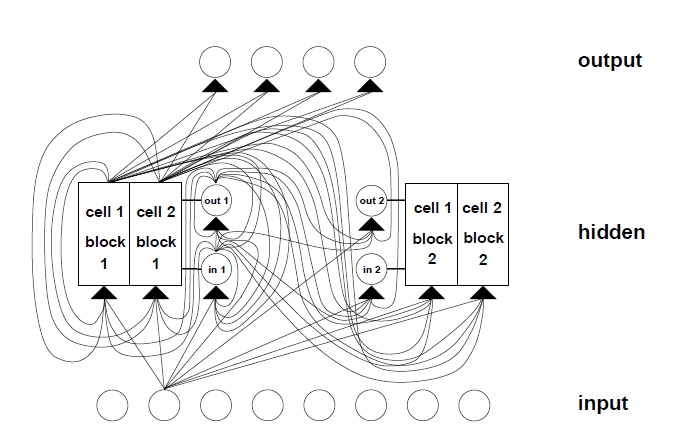
\includegraphics[width=0.7\textwidth]{ figures/estadoarte/lstm_net.PNG}
		\caption{Red LSTM. Imagen obtenida de~\cite{hochreiter1997long}.
		}
		\label{fig.lstm_net}
	\end{center}
\end{figure}
\vspace{-10pt}

Los trabajos expuestos anteriormente dan lugar a la definición de una serie de estructuras dinámicas que permiten abordar con aprendizaje profundo la tarea de la predicción.

\section{Predicción de valores}
El uso de secuencias de valores para la predicción mediante el uso de \acrshort{rna} marca la primera vía de investigación en esta tarea. Así mismo, actualmente es la vía más desarrollada y que presenta muchos de los ejemplos existentes.\\

En el año 2002, miembros del \textit{Institute of Electrical and Electronics Engineers} llevaron a cabo un estudio~\cite{arimaprices} en el se desarrolla un método para predecir los precios de la electricidad al día siguiente según los modelos \acrfull{arima}. Este tipo de modelos se basan en el uso de una serie de procesos estocásticos para analizar series de tiempo, y fue introducida por Box y Jenkins~\cite{box1994series}. El estudio propone dos modelos de este tipo para predecir los precios en cada hora para los mercados eléctricos de España y California, que alcanzan resultados satisfactorios. De entre las conclusiones a las que llega esta investigación cabe destacar que el histórico temporal necesario para realizar la predicción de una forma satisfactoria varía según el mercado, siendo mayor en el español. Además, se plantea el uso de variables explicativas que permiten mejorar los resultados en aquellos meses con una alta correlación entre la producción hidroeléctrica disponible y el precio de la electricidad.\\

En relación con el trabajo anterior, otro estudio que hace uso de los modelos \acrshort{arima} es el desarrollado por G. Peter Zhang~\cite{arimann}, en el que se propone combinar dichos modelos con las \acrshort{rna} para distintas secuencias de valores. El desarrollo de un modelo híbrido viene motivado por la naturaleza combinada de las series temporales: es difícil determinar si una serie de tiempo se genera a partir de un proceso subyacente lineal o no lineal. Con un modelo híbrido se tiene la flexibilidad para modelar una variedad de problemas aprovechando la fuerza en la correlación lineal de \acrshort{arima} y en la no lineal de las \acrshort{rna}. El estudio concluye que, efectivamente, un modelo híbrido ofrece mejores prestaciones que cada modelo por separado, sin embargo la diferencia no es demasiado significativa, según se muestra en la Figura~\ref{fig.arimann}.\\

\begin{figure}[H]
	\begin{center}
		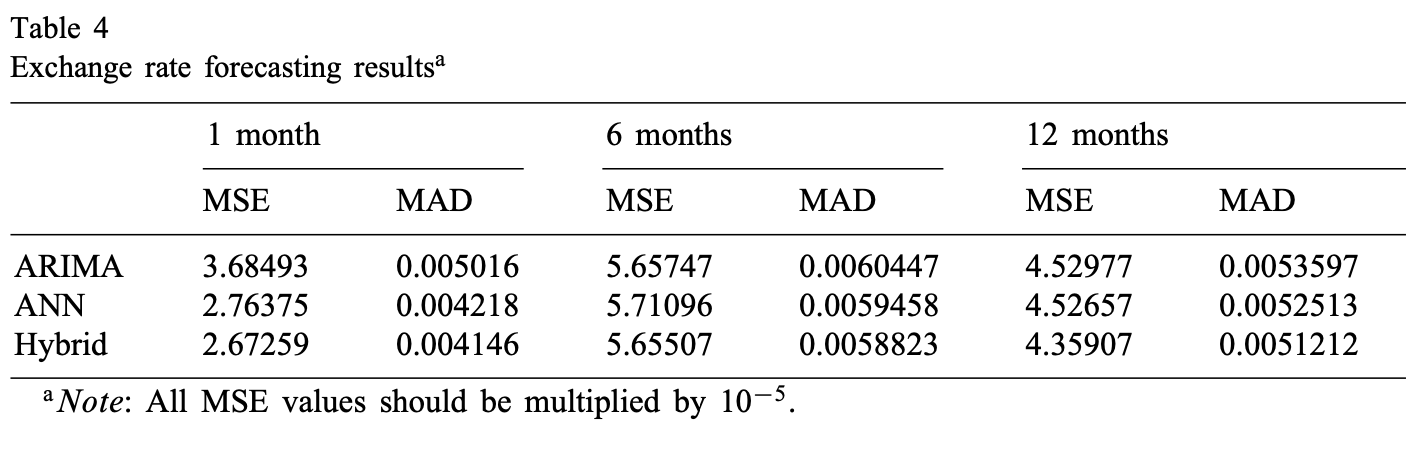
\includegraphics[width=0.85\textwidth]{ figures/estadoarte/ARIMA+NN.png}
		\caption{Resultados comparativos de \acrshort{arima}, \acrshort{rna} y \acrshort{arima}+\acrshort{rna}. Imagen obtenida de~\cite{arimann}.
		}
		\label{fig.arimann}
	\end{center}
\end{figure}
\vspace{-10pt}

Un estudio similar es el desarrollado por un grupo de investigadores japoneses en el año 2015~\cite{dbnARIMA}. En dicho trabajo se combina los modelos \acrshort{arima} con un tipo de red estocástica llamada \acrfull{rbm} seguida de un \acrshort{mlp}. En la Figura~\ref{fig.dbnarima} se muestra el flujo del modelo propuesto, en el que se integran los dos modelos. Se sitúa el foco de la investigación en cómo afecta el orden de ambos modelos en la predicción de distintos valores económicos. El estudio concluye que el orden adecuado depende del tipo de datos con el que se esté trabajando.
\vspace{10pt}
\begin{figure}[H]
	\begin{center}
		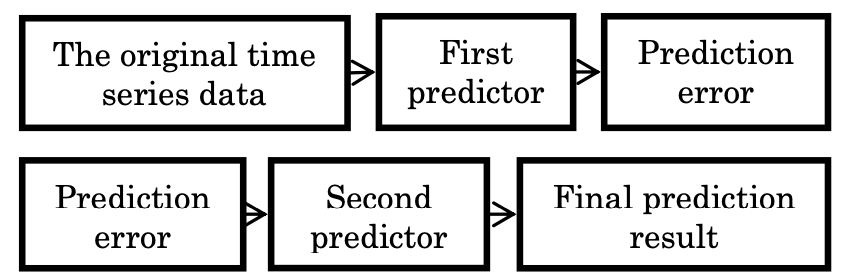
\includegraphics[width=0.5\textwidth]{ figures/estadoarte/flujo_dbn.png}
		\caption{Diagrama de flujo del estudio~\cite{dbnARIMA}.
		}
		\label{fig.dbnarima}
	\end{center}
\end{figure}
\vspace{-10pt}

Respecto al uso de redes recurrentes, Erol Egrioglu, Ufuk Yolcu, Cagdas Hakan Aladag y Eren Basen desarrollan un estudio en el que se propone una arquitectura combinada de \acrshort{rnn} y \acrshort{rna}~(RMNM-ANN)~\cite{multiplicative}. La \acrshort{rnn} propuesta se basa en el modelo de neuronas multiplicativas que se caracterizan por el uso de funciones de agregación multiplicativas en lugar de aditivas. El nuevo modelo, representado en la Figura~\ref{fig.rmnm-ann}, puede producir variables de error rezagadas y utilizarlas como entradas gracias a su estructura de retroalimentación recurrente, y hace uso de una única neurona en la capa oculta de la \acrshort{rna}. El modelo propuesto se aplicó para estimar la cantidad de dióxido de carbono medida mensualmente en Ankara entre marzo de 1995 y abril de 2006, proporcionando mejores resultados que otros modelos de la literatura.

\vspace{10pt}
\begin{figure}[H]
	\begin{center}
		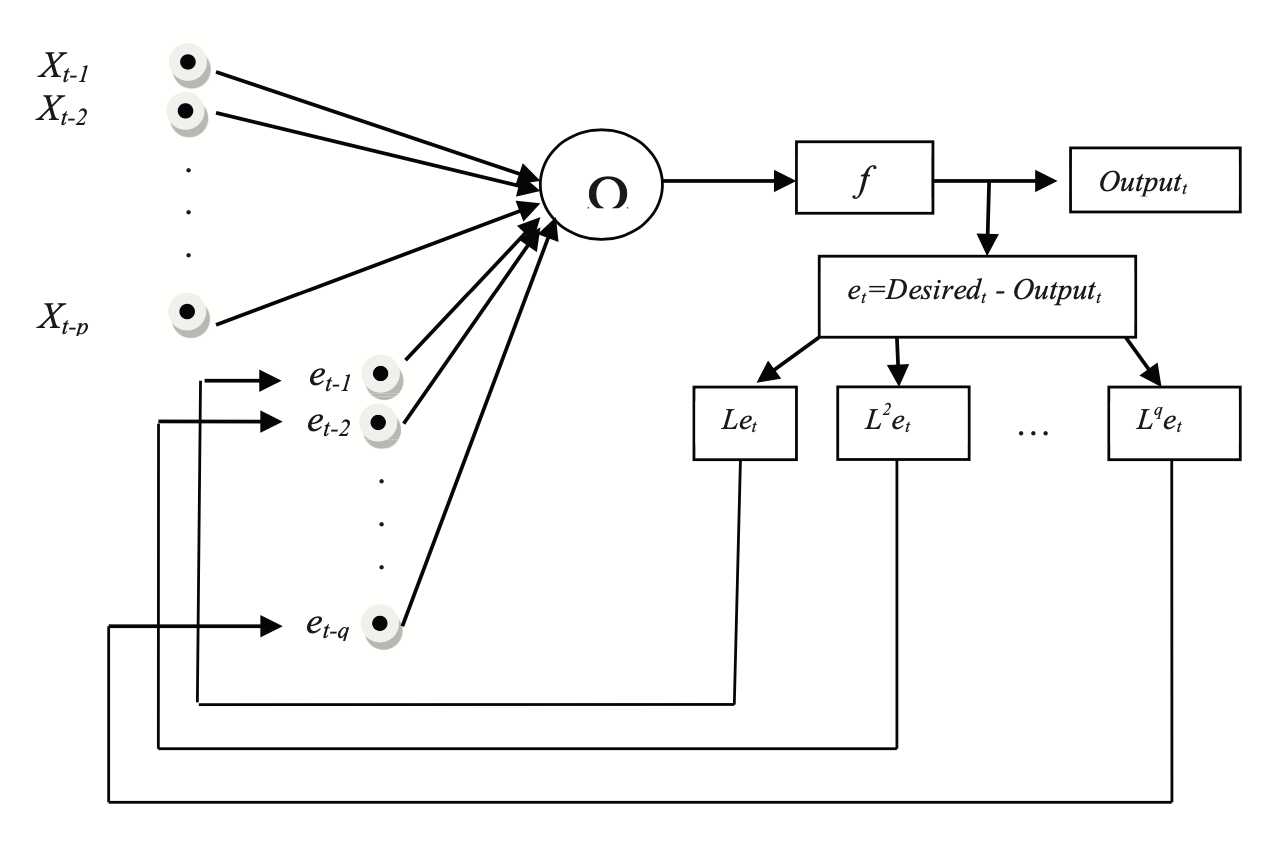
\includegraphics[width=0.51\textwidth]{ figures/estadoarte/rmnm-ann.png}
		\caption{Estructura de RMNM-ANN~\cite{multiplicative}.
		}
		\label{fig.rmnm-ann}
	\end{center}
\end{figure}
\vspace{-10pt}

Algunos estudios han utilizado una combinación de datos de distinta naturaleza para lograr una predicción más precisa. A modo de ejemplo, un artículo de 2018  combina datos temporales con información en forma de texto no estructurado para estimar la demanda de taxi en la ciudad de Nueva York~\cite{taxi}. Para ello se proponen dos estructuras, utilizando una red para el texto y otra para la información temporal y que conjuntamente logran superar de modo significativo a otros métodos populares. La principal diferencia entre ambas estructuras se encuentra en la red utilizada para el procesamiento de la información temporal, que puede ser \acrshort{lstm}~(véase la Figura~\ref{fig.taxi}) o \textit{fully connected}.

\vspace{10pt}
\begin{figure}[H]
	\begin{center}
		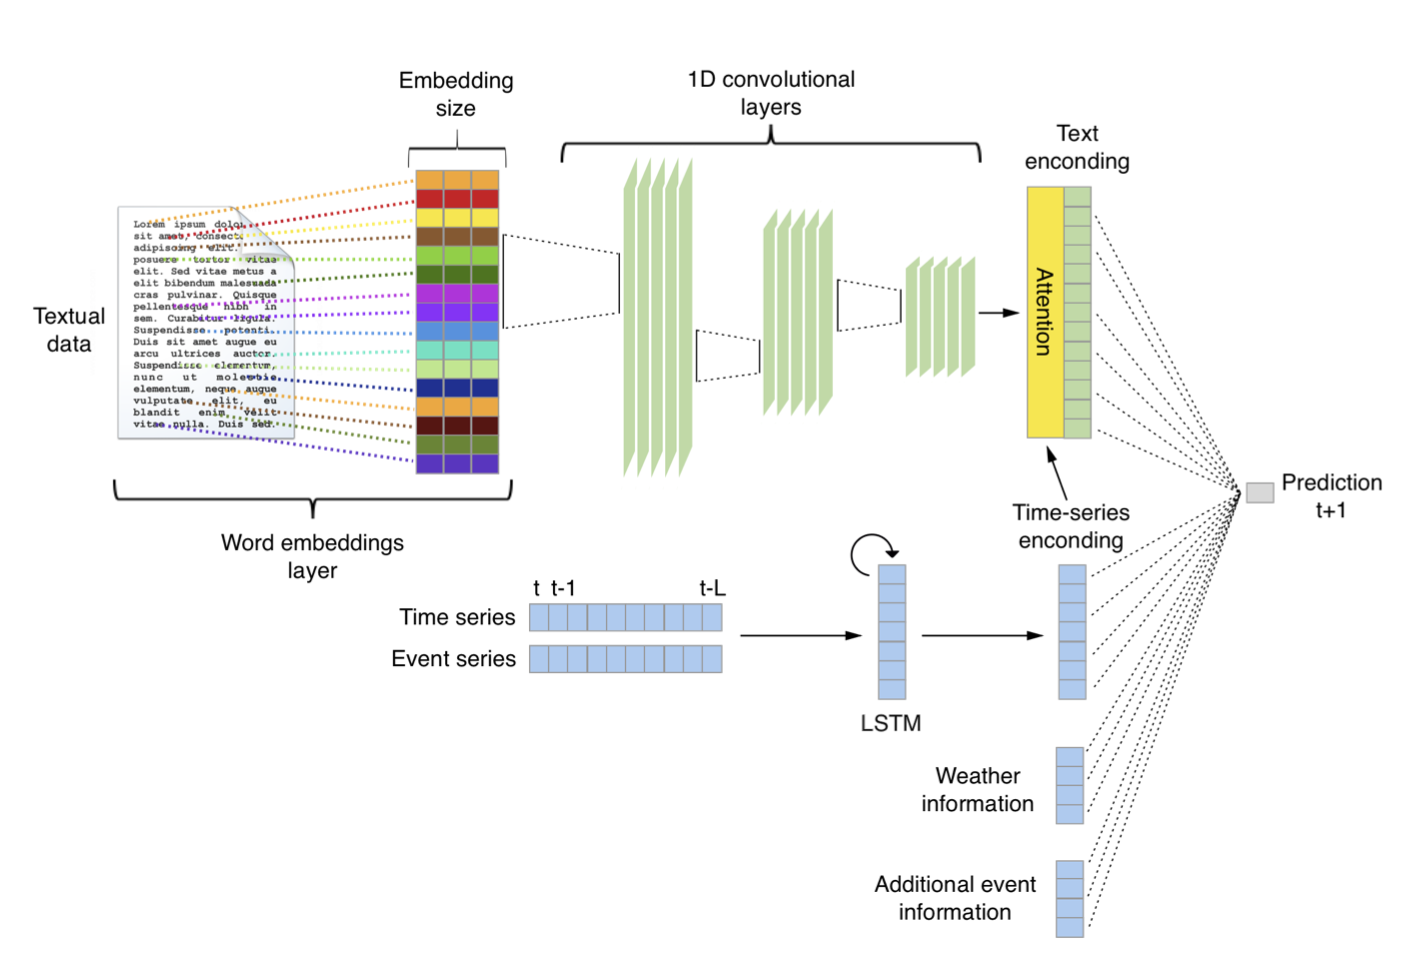
\includegraphics[width=0.95\textwidth]{ figures/estadoarte/taxi.png}
		\caption{Estructura propuesta por~\cite{taxi} con \acrshort{lstm}.
		}
		\label{fig.taxi}
	\end{center}
\end{figure}
\vspace{-10pt}

Finalmente, en cuanto al seguimiento de trayectorias, se han llevado a cabo varios estudios. En el año 2016, se presentó en un artículo la red \textit{SocialLSTM}, cuyo objetivo es lograr es predecir la dinámica del movimiento de peatones en escenas abarrotadas. Esta red es capaz de predecir de forma conjunta las trayectorias de todas las personas que aparecen en una escena teniendo en cuenta las reglas de sentido común y las convenciones sociales que los humanos utilizan mientras se desplazan. Se utiliza una \acrshort{lstm} independiente para cada trayectoria y, posteriormente, se conectan todas ellas a través de una capa de agrupación social (\textit{S-pooling}), compartiendo información entre sí. En la Figura~\ref{fig.socialstm} se muestra la estructura de la red propuesta. El método propuesto logra superar a los métodos de vanguardia en dos conjuntos de datos públicos~(ETH y UCY). Además, es capaz de predecir con éxito varios comportamientos no lineales que surgen de interacciones sociales. 

\vspace{10pt}
\begin{figure}[H]
	\begin{center}
		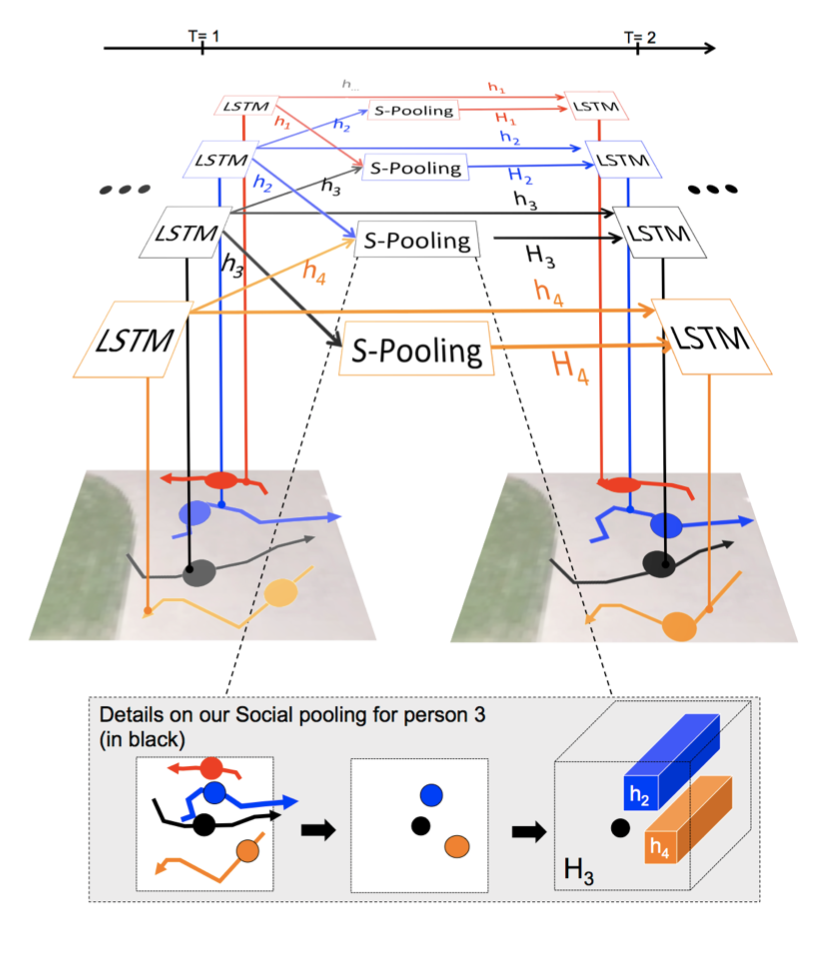
\includegraphics[width=0.7\textwidth]{ figures/estadoarte/sociallstm.png}
		\caption{Estructura de SocialLSTM~\cite{sociallstm}.
		}
		\label{fig.socialstm}
	\end{center}
\end{figure}
\vspace{-10pt}



Otro estudio en relación con trayectorias, en esta ocasión de vehículos~\cite{vehicletrajectory}, se publica en el 2018 y se basa en la arquitectura de red neuronal del codificador-decodificador \textit{lstm}\footnote{\url{https://machinelearningmastery.com/encoder-decoder-long-short-term-memory-networks/}}. El sistema propuesto, mostrado en la Figura~\ref{fig.vehicletrajectory}, se basa en el análisis de varias observaciones pasadas del vehículo por el codificador para que el decodificador genere un número \textit{K} de posibles trayectorias a seguir. Este método es capaz de lograr una mejora significativa con respecto a los métodos existentes en términos de precisión de predicción, al mismo tiempo que puede generar la secuencia completa de la trayectoria predicha.

\vspace{10pt}
\begin{figure}[H]
	\begin{center}
		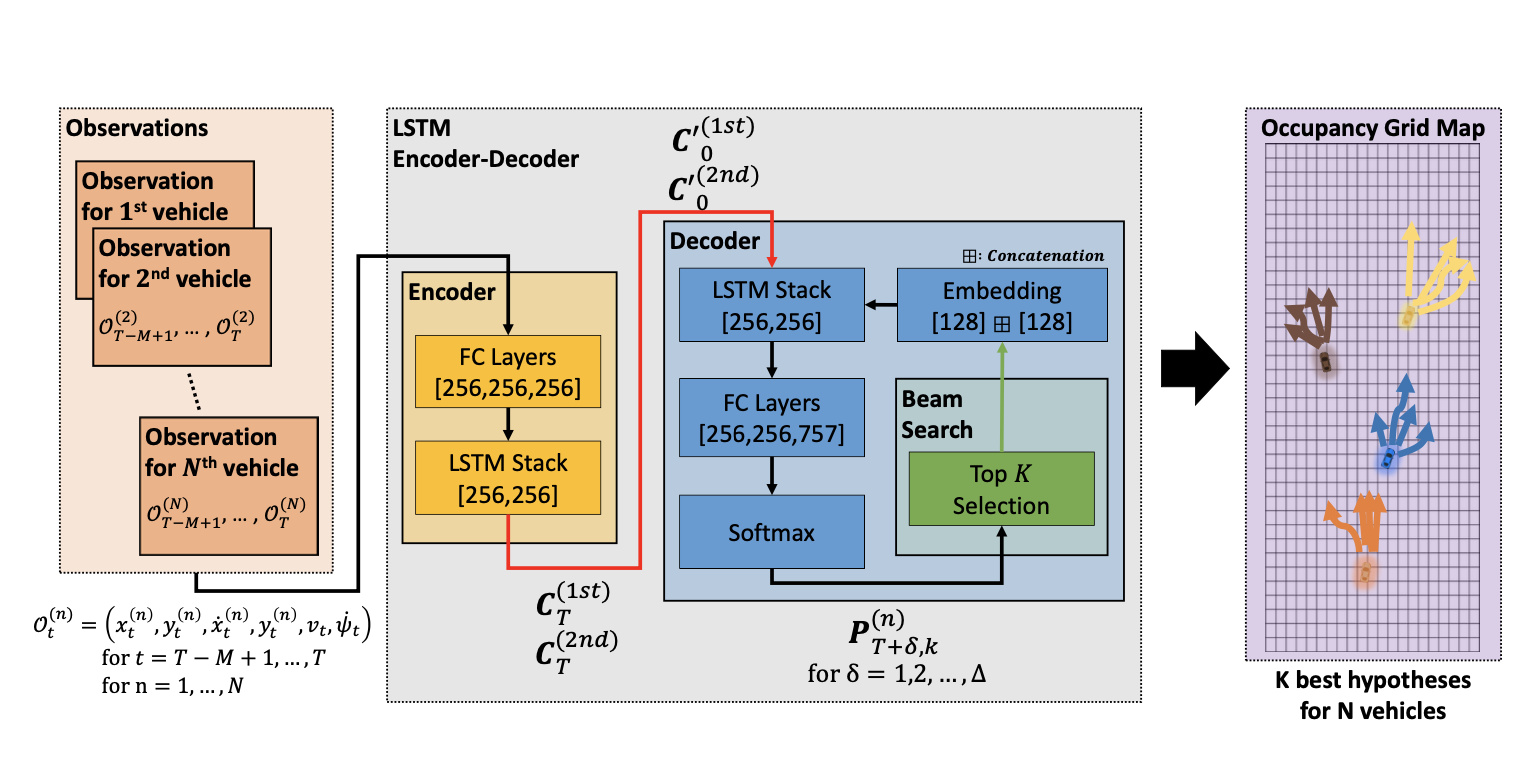
\includegraphics[width=0.95\textwidth]{ figures/estadoarte/vehicle_trajectory.png}
		\caption{Estructura propuesta por~\cite{vehicletrajectory}.
		}
		\label{fig.vehicletrajectory}
	\end{center}
\end{figure}
\vspace{-10pt}

\section{Predicción en imágenes}
La investigación en la tarea de predicción con secuencias de imágenes o de vídeo está menos desarrollada, puesto que surge más tarde que para las secuencias numéricas.\\

Uno de los campos en los que se han realizado estudios de predicción con imágenes es el de los videojuegos. En el año 2015 se publica un artículo~\cite{actiongames} que propone dos estructuras, mostradas en la Figura~\ref{fig.games_nets}, novedosas hasta el momento para la predicción de fotogramas que dependen de las acciones del jugador. Los resultados, tanto cualitativos como cuantitativos, muestran que ambas redes son capaces de predecir fotogramas visualmente realistas y útiles para el control del juego, con una separación temporal~(\textit{gap}) de 100 pasos en varios juegos de Atari de distinto dominio. Se trata de uno de los primeros artículos que muestra buenas predicciones en los juegos de Atari.\\

\vspace{10pt}
\begin{figure}[H]
	\begin{center}
		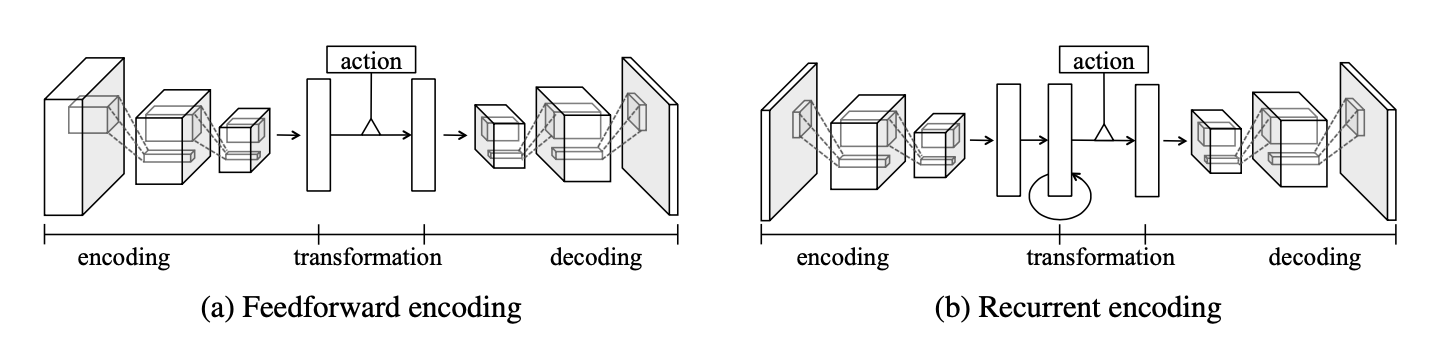
\includegraphics[width=0.95\textwidth]{ figures/estadoarte/games_nets.png}
		\caption{Estructuras propuestas en~\cite{actiongames}.
		}
		\label{fig.games_nets}
	\end{center}
\end{figure}
\vspace{-10pt}

Otro campo de estudio es la predicción de secuencias de vídeo, anticipándose a las acciones que sucederán en la secuencia. Un ejemplo de ello es el artículo propuesto por Carl Vondrick, Hamed  Pirsiavash y Antonio Torralba, que se centra en dicha predicción mediante aprendizaje no supervisado~\cite{unlabeledvideo}. Se propone la estructura definida en la Figura~\ref{fig.unlabeled_net}, entrenada con más de 600 horas de vídeo de \textit{YouTube} con diferentes temáticas. Con las predicciones obtenidas realizan una clasificación de la acción que se está desarrollando en la escena, obteniendo resultados bastante satisfactorios aunque con margen de mejora.

\vspace{10pt}
\begin{figure}[H]
	\begin{center}
		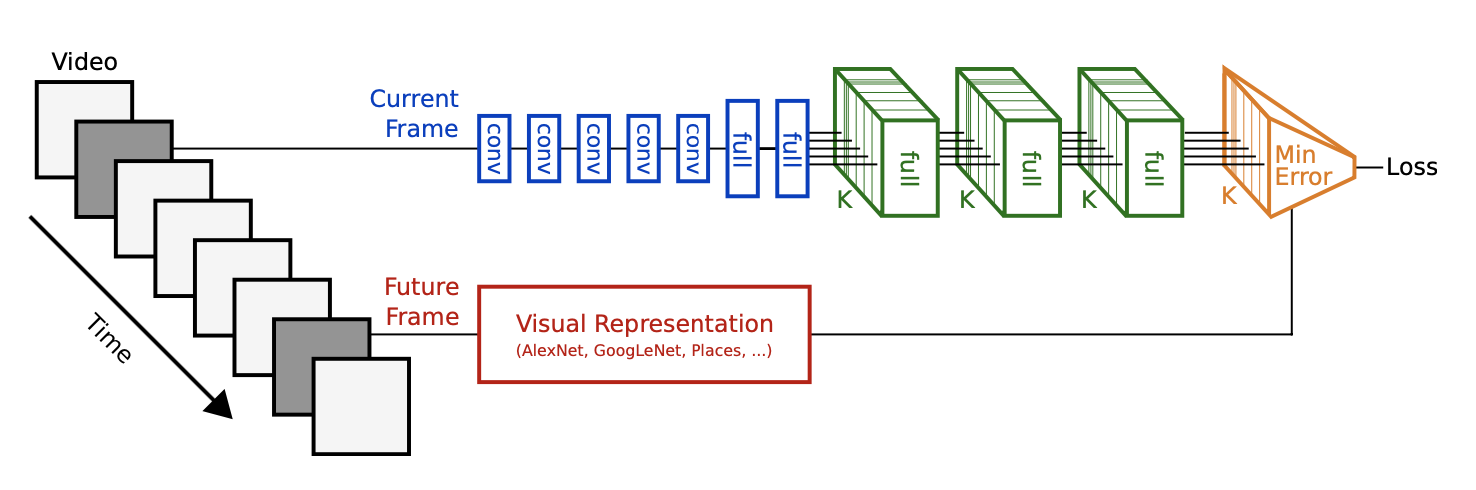
\includegraphics[width=0.95\textwidth]{ figures/estadoarte/unlabeled_net.png}
		\caption{Estructura propuesta en~\cite{unlabeledvideo}.
		}
		\label{fig.unlabeled_net}
	\end{center}
\end{figure}
\vspace{-10pt}

En en año 2018 se publica un estudio que propone la descomposición del movimiento y el contenido para manejar de forma efectiva la evolución los píxeles en los vídeos~\cite{descompose}. El modelo propuesto~(MCnet), mostrado en la Figura~\ref{fig.descompose}, se basa en un codificador-decodificador con \acrshort{cnn} y una \acrshort{lstm} convolucional que obtiene la predicción a nivel de píxel. Debido a la separación entre movimiento y contenido, la predicción se obtiene convirtiendo el contenido extraído en el contenido del siguiente fotograma mediante las características de movimiento identificadas, simplificando la tarea. Para evaluar la red y compararla con otras estructuras han empleado los conjuntos de datos KTH, Weizmann action y UCF-101, que están formados por vídeos de actividad de personas. La estructura propuesta es considerada una de las primeras arquitecturas que realizan la separación de movimiento y contenido en la predicción a nivel de píxeles en vídeos naturales.\\

\vspace{10pt}
\begin{figure}[H]
	\begin{center}
		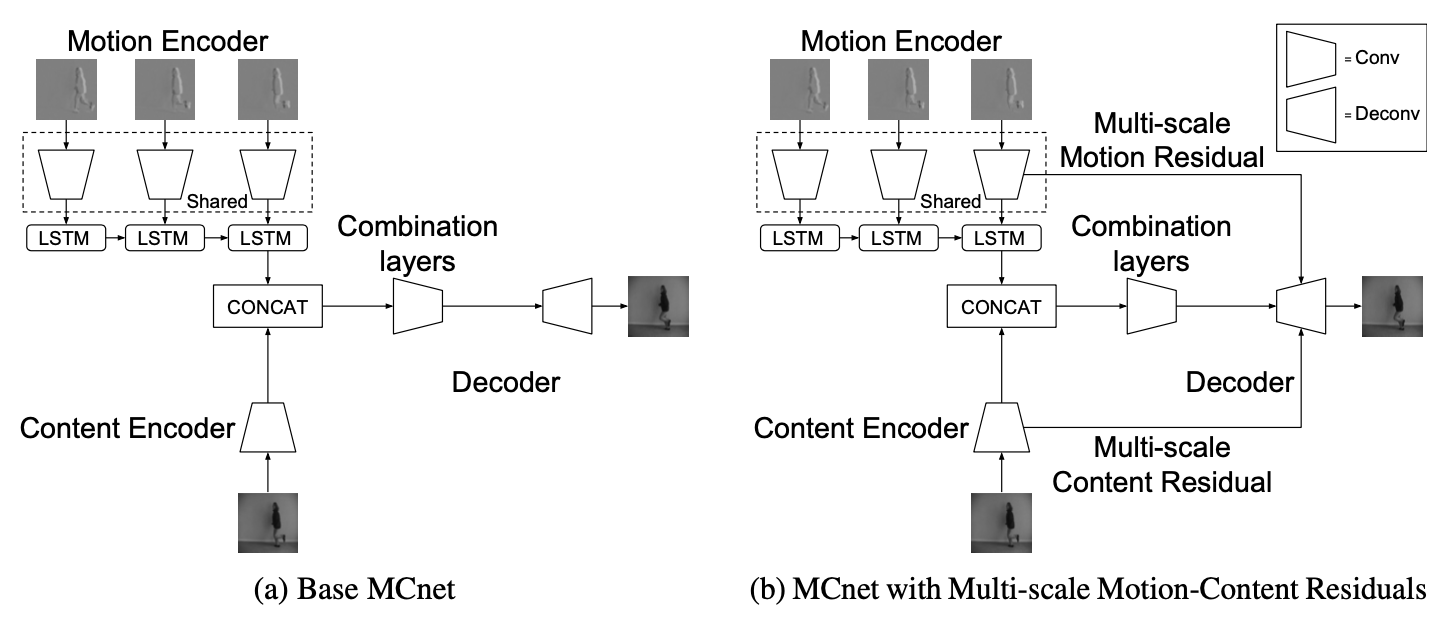
\includegraphics[width=0.95\textwidth]{ figures/estadoarte/descompose.png}
		\caption{Estructura de red MCnet~\cite{descompose}.
		}
		\label{fig.descompose}
	\end{center}
\end{figure}
\vspace{-10pt}

En el año 2019, Jason Y. Zhang, Panna Felsen, Angjoo Kanazawa y Jitendra Malik llevaron a cabo un estudio para predecir el movimiento 3D de una persona a partir de una secuencia de vídeo~\cite{3d}. Es uno de los primeros enfoques que tratan de predecir una malla 3D a partir de una serie de fotogramas, por lo que el margen de mejora es todavía bastante amplio. Este modelo~(PHD) centra su atención en acciones periódicas como el caminar, lanzar a los bolos o realizar un ejercicio de gimnasio. En la Figura~\ref{fig.3d} se muestra un ejemplo de funcionamiento. 

\vspace{10pt}
\begin{figure}[H]
	\begin{center}
		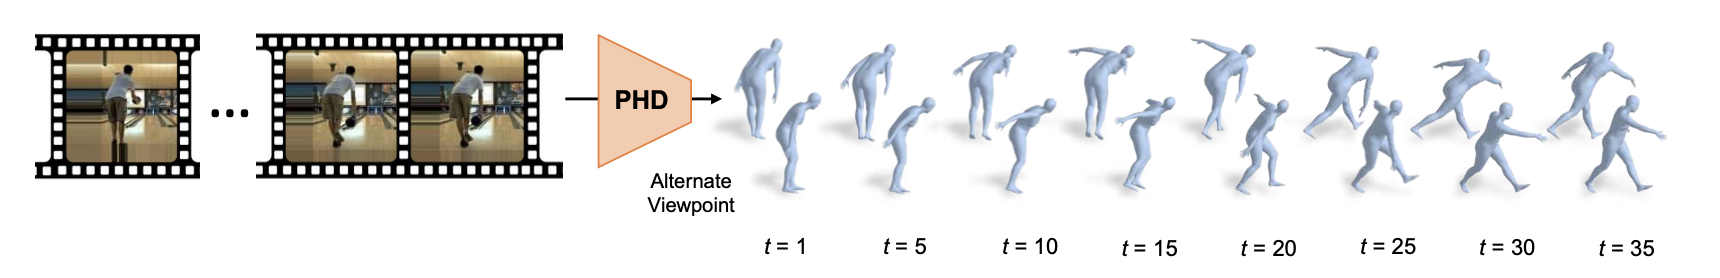
\includegraphics[width=1\textwidth]{ figures/estadoarte/3D-func.png}
		\caption{Funcionamiento de PHD~\cite{3d}.}
		\label{fig.3d}
	\end{center}
\end{figure}
\vspace{-10pt}

La arquitectura definida se basa en modelos autorregresivos y no necesita de vídeos etiquetados en 3D, se puede entrenar con vídeos que sólo dispongan de anotaciones 2D. El modelo desarrollado en este estudio, mostrado en la Figura~\ref{fig.3d_net}, está formado por cuatro partes:
\begin{itemize}
    \item Una \textit{Resnet} que se encarga de extraer las características de cada fotograma.
    \item Un codificador temporal causal que aprende una ``tira de película'', es decir, una representación latente de la dinámica humana en 3D.
    \item Un regresor 3D que puede leer la malla 3D de la tira de película.
    \item Un modelo autorregresivo en el espacio latente que toma las tiras de películas pasadas para predecir las películas futuras, capturando así la dinámica humana.
\end{itemize}

\vspace{10pt}
\begin{figure}[H]
	\begin{center}
		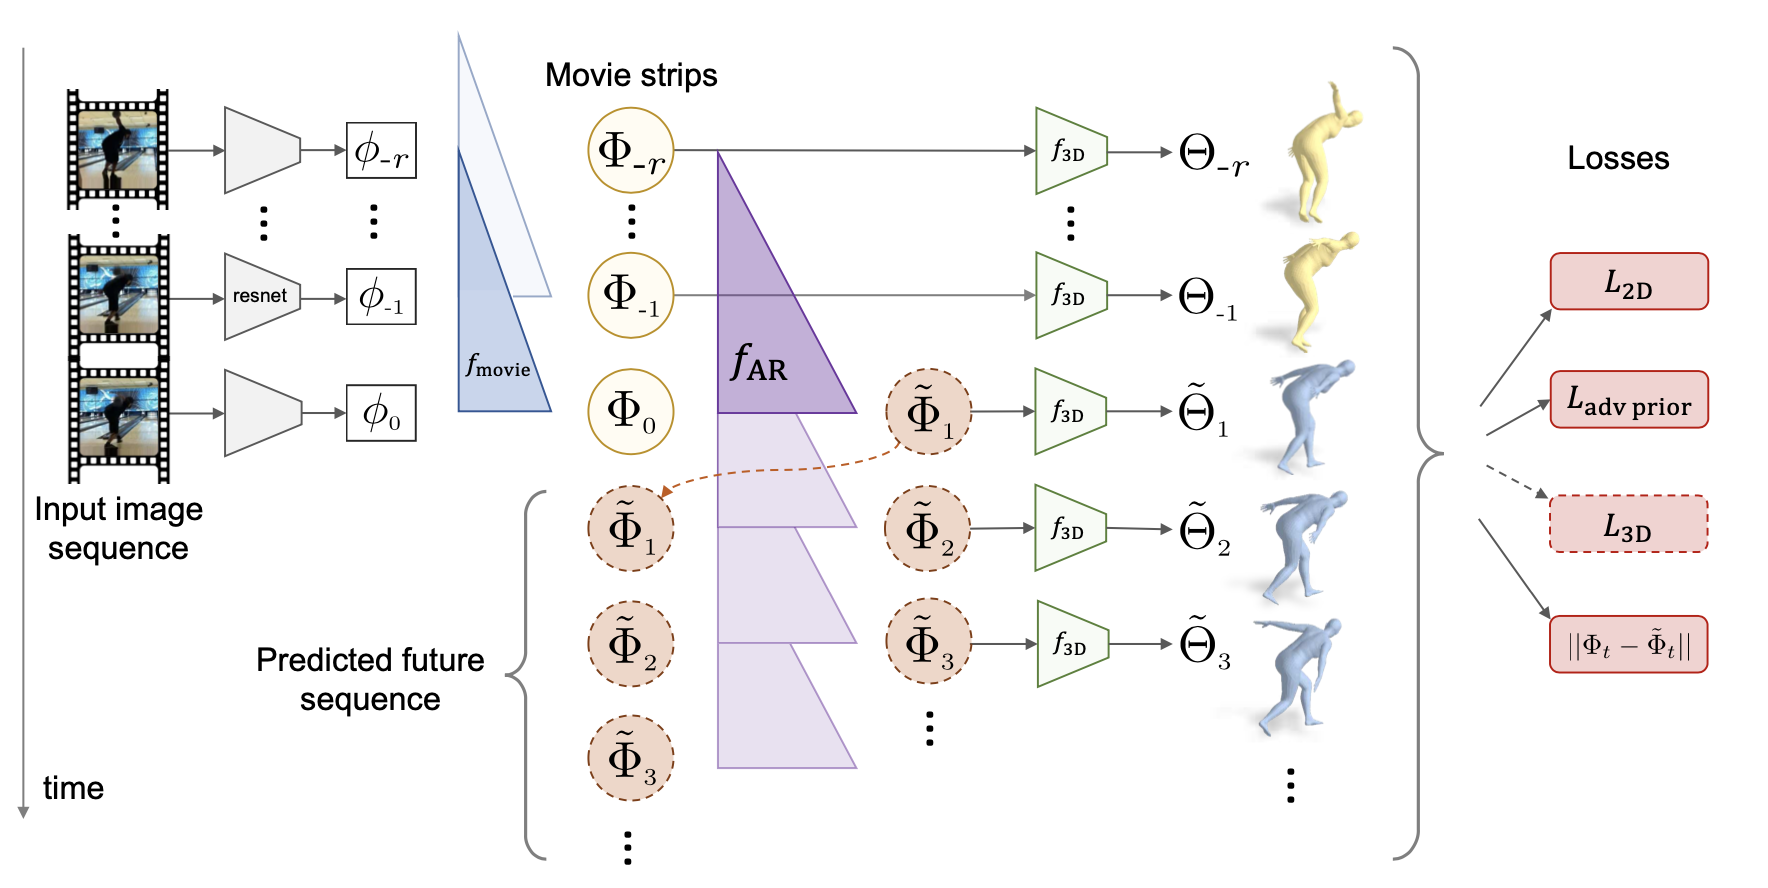
\includegraphics[width=0.95\textwidth]{ figures/estadoarte/3D-net.png}
		\caption{Estructura de red PHD~\cite{3d}.}
		\label{fig.3d_net}
	\end{center}
\end{figure}
\vspace{-10pt}

Finalmente, uno de los estudios más recientes~\cite{photorealistic} trata de obtener la predicción del fotograma lo más nítida y realista posible, evitando las distorsiones que generan otros métodos de predicción. Para ello se hace uso de la estructura definida en la Figura~\ref{fig.real-net}, una red residual profunda con arquitectura jerárquica donde cada capa hace una predicción del estado futuro a diferentes resoluciones espaciales para después fusionarlas a través de conexiones de arriba hacia abajo.

\vspace{10pt}
\begin{figure}[H]
	\begin{center}
		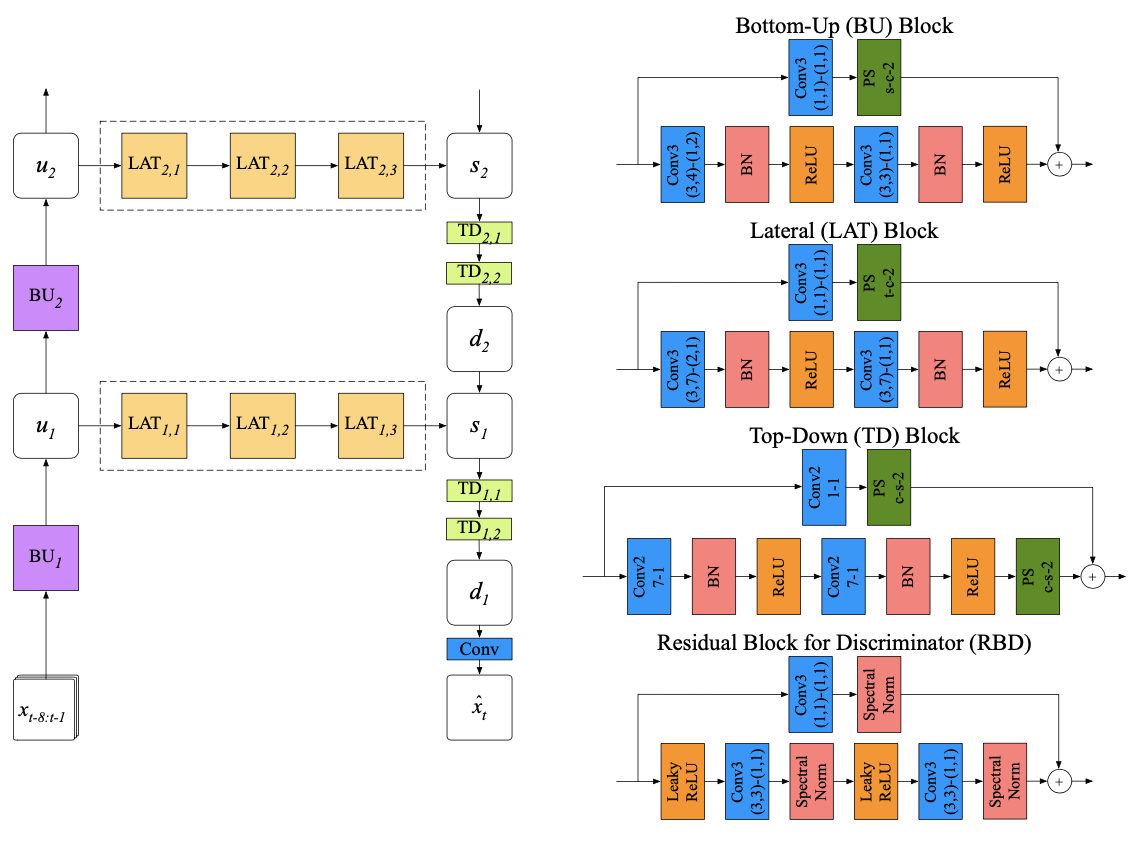
\includegraphics[width=0.85\textwidth]{ figures/estadoarte/Real-net.png}
		\caption{Estructura propuesta en~\cite{photorealistic}.}
		\label{fig.real-net}
	\end{center}
\end{figure}
\vspace{-10pt}

El modelo propuesto supera cuantitativamente las líneas del estado del arte en la predicción de fotogramas futuros y es capaz de generar fotogramas con detalles más finos y texturas que son perceptualmente más realistas, según se muestra en la Figura~\ref{fig.real-func}.

\vspace{10pt}
\begin{figure}[H]
	\begin{center}
		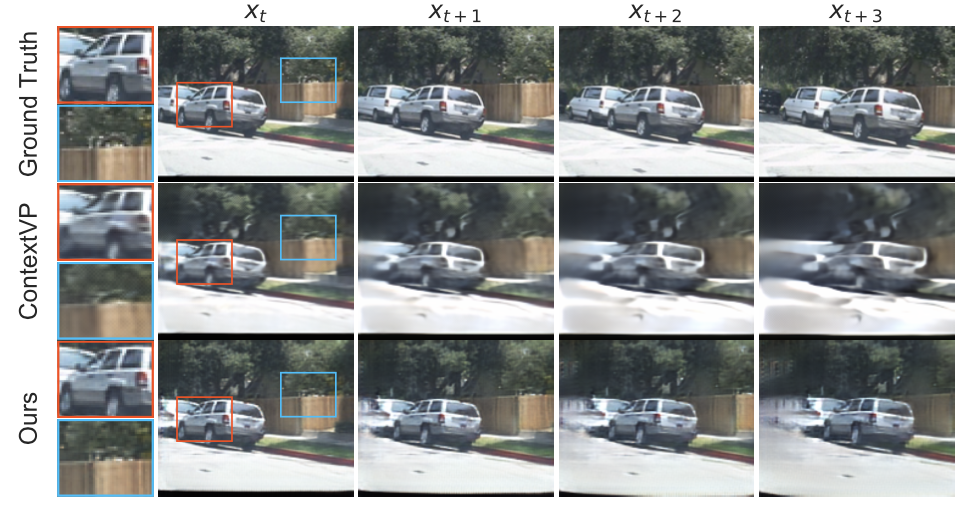
\includegraphics[width=0.85\textwidth]{ figures/estadoarte/Real-func.png}
		\caption{Resultados de estructura propuesta en~\cite{photorealistic}.}
		\label{fig.real-func}
	\end{center}
\end{figure}
\vspace{-10pt}

\section{Infraestructura utilizada}
Esta sección describe los elementos \textit{software} y \textit{hardware} utilizados en el desarrollo de este trabajo. Se explica el lenguaje de programación empleado, las herramientas \textit{software} necesarias, y el servidor en el que se han ejecutado todos los experimentos.

\subsection{Lenguaje Python}
Python\footnote{\url{https://www.python.org}} es un lenguaje de programación orientado a objetos, interpretado e interactivo que combina una alta potencia con una sintaxis muy clara. Esta sencillez en la sintaxis hace que sea fácil de aprender. Además la comunidad de desarrolladores proporciona conferencias, documentación y listas de correo que facilitan su aprendizaje.\\

La potencia de este lenguaje viene dada por la fácil combinación de la biblioteca estándar con miles de módulos de terceros que permite aumentar casi infinitamente el rango de posibilidades de sus aplicaciones. Además, puede ser utilizado como lenguaje de extensión para aplicaciones escritas en otros lenguajes que necesitan interfaces de automatización o \textit{scripts} fáciles de usar. Todo esto hace que su uso se haya extendido en las distintas aplicaciones de \acrshort{ia}. Es un lenguaje de código abierto que permite su libre uso y distribución, cuya licencia está administrada por la \textit{``Python Software Foundation''}.\\

Actualmente, la versión de Python más reciente es la 3.8.6,  lanzada el 24 de septiembre de 2020. Sin embargo, en la realización de este trabajo se ha utilizado la versión 3.6.9, pues era la última en el momento de comenzar el desarrollo.

\subsection{Biblioteca OpenCV}
OpenCV (\textit{Opne Source Computer Vision Library})\footnote{\url{https://opencv.org}} es una librería de código abierto para realizar tareas de \acrshort{va} y aprendizaje automático. Fue creado con el objetivo de facilitar una infraestructura común para diversas aplicaciones de \acrshort{va} y acelerar su uso en productos comerciales.\\

Su uso está muy extendido, pues cuenta con más de 47 mil usuarios en la comunidad y un número aproximado de descargas superior a 18 millones. Su expansión abarca desde grupos de investigación hasta empresas tan potentes como \textit{Google}, y cuenta con algunos usos desplegados como la unión de imágenes en \textit{streetview} o la comprobación de pistas en busca de escombros en Turquía.\\

Presenta interfaces para los lenguajes C++, Java, MATLAB y Python, esta última utilizada en este trabajo. En cuanto a sistemas operativos, es compatible con Windows, Linux, Android y Mac OS. Dispone de más de 2500 algoritmos, clásicos y de última generación, que han sido optimizados y que permiten realizar tareas como la detección de rostros y su identificación, el seguimiento de objetos, la extracción de modelos 3D de los objetos o la búsqueda de patrones.\\

El principal uso de OpenCV en el trabajo se ha centrado en el procesamiento de las imágenes utilizadas para el entrenamiento y la evaluación de las redes mediante tres métodos:

\begin{itemize}
    \item \textbf{\textit{cv2.imwrite(filename, image)}:} Almacena la imagen (\textit{image}) en el fichero (\textit{filename}). Se utiliza en la generación de las imágenes para almacenar las secuencias de imágenes en la base de datos.
    \item \textbf{\textit{cv2.imread(path, flag=0)}:} Lee la imagen almacenada en \textit{path} en escala de grises (\textit{flag=0}). Se utiliza en la lectura las secuencias de imágenes de la base de datos para entrenar o evaluar las distintas redes.
    \item \textbf{\textit{cv2.GaussianBlur(image, (5, 5), 0)}:} Aplica un filtro gaussiano a la imagen para expandir el píxel en una ventana de 5x5. Se utiliza como preprocesamiento de las imágenes en algunos estudios.
\end{itemize}

La versión más reciente de la biblioteca OpenCV en la actualidad es la 4.4.0, mientras que la empleada en este trabajo es la 4.2.0 con su interfaz de Pyhton.

\subsection{Biblioteca Matplotlib}
La librería Matplotlib\footnote{\url{https://matplotlib.org}} está enfocada a la creación de gráficos 2D de matrices en Pyhton. Su origen se sitúa en la emulación de comandos gráficos de MATLAB pero ha desembocado en una biblioteca completamente independiente de este lenguaje que puede ser usada en Python y de forma orientada a objetos. Está escrito principalmente en Python puro, aunque utiliza de forma intensiva la librería Numpy para el tratamiento de matrices, y otros códigos de extensión para un buen rendimiento incluso con matrices grandes. La filosofía de esta biblioteca radica en la capacidad de crear gráficos simples con unos pocos comandos, o tan solo uno.\\

Los usos de Matplotlib son muy variados. En este trabajo se emplean para la representación gráfica de las distintas métricas calculadas para comparar las prestaciones de las diferentes redes. En concreto, se hace uso de dos gráficos:

\begin{itemize}
    \item \textbf{\textit{pyplot.bar}:} Dibuja un diagrama de barras dados un par de vectores \textit{x} e \textit{y} con el mismo número de valores. Permite la modificación de parámetros como el ancho de la barra, su alineación respecto el valor de \textit{x} o el color de la misma.
    \item \textbf{\textit{pyplot.boxplot}:} Dibuja un diagrama de caja y bigotes sobre un conjunto de datos. En este gráfico se representa la caja, con los valores del cuartil inferior al superior de los datos con una línea en la mediana; y los bigotes, que se extienden desde la caja para mostrar el rango de los datos. Además aparecen representados los distintos \textit{outliers} como puntos más allá del final de los bigotes.
\end{itemize}

La versión más reciente de Matplotlib es la 3.3.2, pero en este trabajo se hace uso de la versión 3.1.3.

\subsection{Middleware neuronal Keras}
Keras\footnote{\url{https://keras.io}} es un \textit{middleware} de aprendizaje profundo escrito en Python que se ejecuta sobre la plataforma Tensorflow. Su enfoque de desarrollo se sitúa en lograr una experimentación rápida, pasando de la idea al resultado de una forma fluida. Keras es la API de alto nivel de TensorFlow 2.0 que proporciona abstracciones y bloques de construcción esenciales para desarrollar diversas soluciones de aprendizaje automático con una alta velocidad de iteración.\\

Las estructuras de datos centrales de este \textit{middleware}, sobre las que se entrará en detalle a continuación, son los llamados modelos y capas.

\subsubsection{Modelos en Keras}
Un modelo es una estructura de datos que engloba a otras, las capas, para la creación de redes neuronales de aprendizaje profundo. El tipo de modelo más sencillo definido en Keras, y el utilizado en este trabajo, es el \textit{Sequential()} que apila todas las capas de forma lineal. Para trabajar con estos modelos se utilizan las funciones que se exponen a continuación:

\begin{itemize}
    \item \textbf{\textit{model.add(layer)}:} Se utiliza para añadir una nueva capa (\textit{layer}) al modelo (\textit{model}).
    \item \textbf{\textit{model.compile(...)}:} Sirve para, una vez definida la estructura, configurar la red para el entrenamiento. A esta función se le pueden pasar varios argumentos, siendo empleados en este trabajo dos de ellos:
    \begin{itemize}
        \item \textit{loss}: Define la función de pérdida a optimizar y varía según el experimento a realizar.
        \item \textit{optimizer}: Define el tipo de optimizador a utilizar.
    \end{itemize}
    \item \textbf{\textit{model.fit(...)}:} Entrena el modelo bajo una serie de condiciones. Los parámetros utilizados son:
    \begin{itemize}
        \item \textit{x}: Datos de entrenamiento.
        \item \textit{y}: Etiquetas de entrenamiento.
        \item \textit{batch}\_\textit{size}: Tamaño del lote, número de muestras utilizadas en cada actualización de gradiente.
        \item\textit{epochs}: Número de épocas a entrenar.
        \item \textit{validation}\_\textit{data}: Datos de validación.
        \item \textit{callbacks}: Lista con los objetos para realizar acciones en varias etapas del entrenamiento. En concreto se hace uso de dos de ellos.
        \begin{itemize}
            \item \textit{early}\_\textit{stopping}: Define un criterio de parada en el entrenamiento cuando el valor de la función de \textit{loss} no mejora un número de épocas consecutivas.
            \item \textit{checkpoint}: Guarda el modelo en un punto de control determinado. En este trabajo, se guarda el modelo si éste es mejor que el anterior en términos de \textit{loss} con el conjunto de validación.
        \end{itemize}
        \item \textit{verbose}: Establece la forma de obtener información sobre el entrenamiento del modelo durante el avance del mismo.
    \end{itemize}
    \item \textbf{\textit{model.fit}}\_\textbf{\textit{generator(...)}:} Realiza la misma operación que el \textit{fit} pero con una división por lotes del conjunto de entrenamiento. Se utilizan los mismos parámetros que los definidos en la función anterior salvo tres de variaciones:
    \begin{itemize}
        \item \textit{generator}: Especifica la forma en la que se obtienen los distintos lotes para el entrenamiento. Para este trabajo se trata de una función que lee un bloque de secuencias del tamaño indicado. Esta función sustituye a los valores de \textit{x} e \textit{y}.
        \item \textit{steps}\_\textit{per}\_\textit{epoch}: Establece el número de lotes que se procesarán en cada época. Este valor se obtiene como \textit{Tamaño conjunto entrenamiento / Tamaño lote}.
        \item \textit{validation}\_\textit{steps}: Establece el número de lotes que se validarán en cada época. Este valor se obtiene como \textit{Tamaño conjunto validación / Tamaño lote}.
    \end{itemize}
    \item \textbf{\textit{model.predict(dataX)}:} Genera las predicciones sobre los datos de entrada que se proporcionen~(\textit{dataX}).
    
\end{itemize}
Por último, para poder obtener una representación esquemática de la estructura de la red diseñada se hace uso del método \textit{utils.vis}\_\textit{utils.plot}\_\textit{model(model, path)} que almacena la estructura del modelo (\textit{model}) en la ruta definida (\textit{path}). Por otro lado, la función \textit{models.load}\_\textit{model(path)} carga en memoria un modelo de Keras previamente guardado.

\subsubsection{Capas en Keras}
Como se mencionó anteriormente, los modelos en Keras están compuestos por una combinación de varias de sus capas. A continuación se exponen las capas utilizadas en este trabajo, un subconjunto de todas las posibilidades que proporciona el API.

\begin{itemize}
    \item \textbf{\textit{Dense}:} Define una capa completamente conectada (\textit{fully connected}) con un número de neuronas determinado.
    \item \textbf{\textit{Conv2D}:} Se trata de una capa de convolución en la que un núcleo~(\textit{kernel}) convoluciona con la entrada de la capa para producir un tensor de salidas.
    \item \textbf{\textit{MaxPooling2D}:} Es una capa que realiza una operación de agrupación máxima para datos espaciales 2D. Reduce la representación de entrada utilizando el valor máximo sobre una ventana de tamaño definido en el parámetro \textit{pool}\_\textit{size}. 
    \item \textbf{\textit{LSTM}:} Crea una capa recurrente de tipo LSTM con un número de celdas de memoria determinado y la posibilidad de devolver las secuencias para apilar varias capas de este tipo.
    \item \textbf{\textit{ConvLSTM2D}:} Establece una capa de tipo ConvLSTM en dos dimensiones, en la que las multiplicaciones en una celda de memoria se sustituyen por operadores de convolución.
    \item \textbf{\textit{Flatten}:} Se trata de una capa cuya función es reestructurar la entrada que recibe como un vector unidimensional.
    \item \textbf{\textit{TimeDistributed}:} No es una capa como tal. Se trata de un contenedor que permite aplicar una capa a cada segmento temporal de una entrada. La entrada debe ser al menos 3D, y la primera dimensión será considerada la dimensión temporal.
\end{itemize}

En todas estas capas se definen el número de neuronas que tiene cada capa y la función de activación a utilizar, encargada de normalizar el valor de la salida en un rango determinado. Para este trabajo han sido consideradas cuatro funciones de activación, representadas en la Figura~\ref{fig.activacion}.

\begin{figure}[H]
		\begin{center}
			\subfigure[]{
\includegraphics[width=0.3\textwidth]{ figures/estadoarte/lineal.png}} \hspace{10pt}
	        \subfigure[]{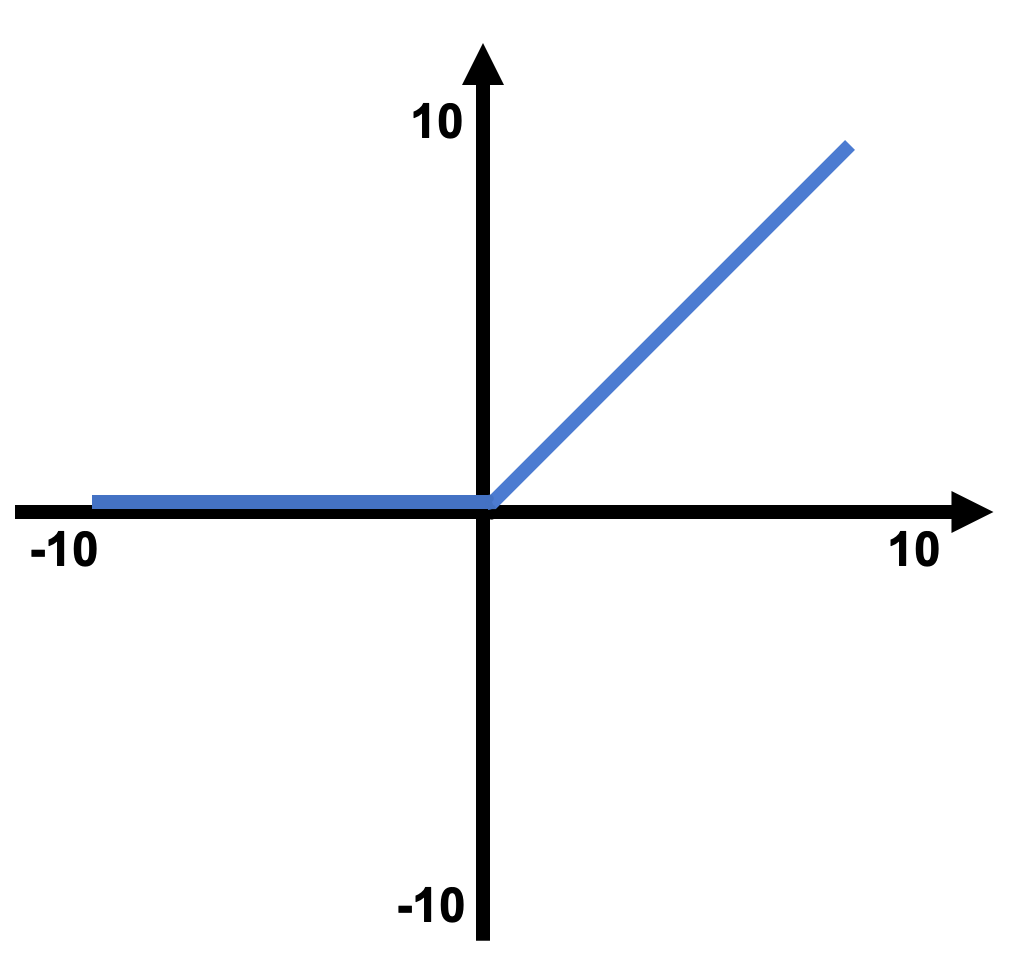
\includegraphics[width=0.3\textwidth]{ figures/estadoarte/relu.png}} \vskip\baselineskip
	        \subfigure[]{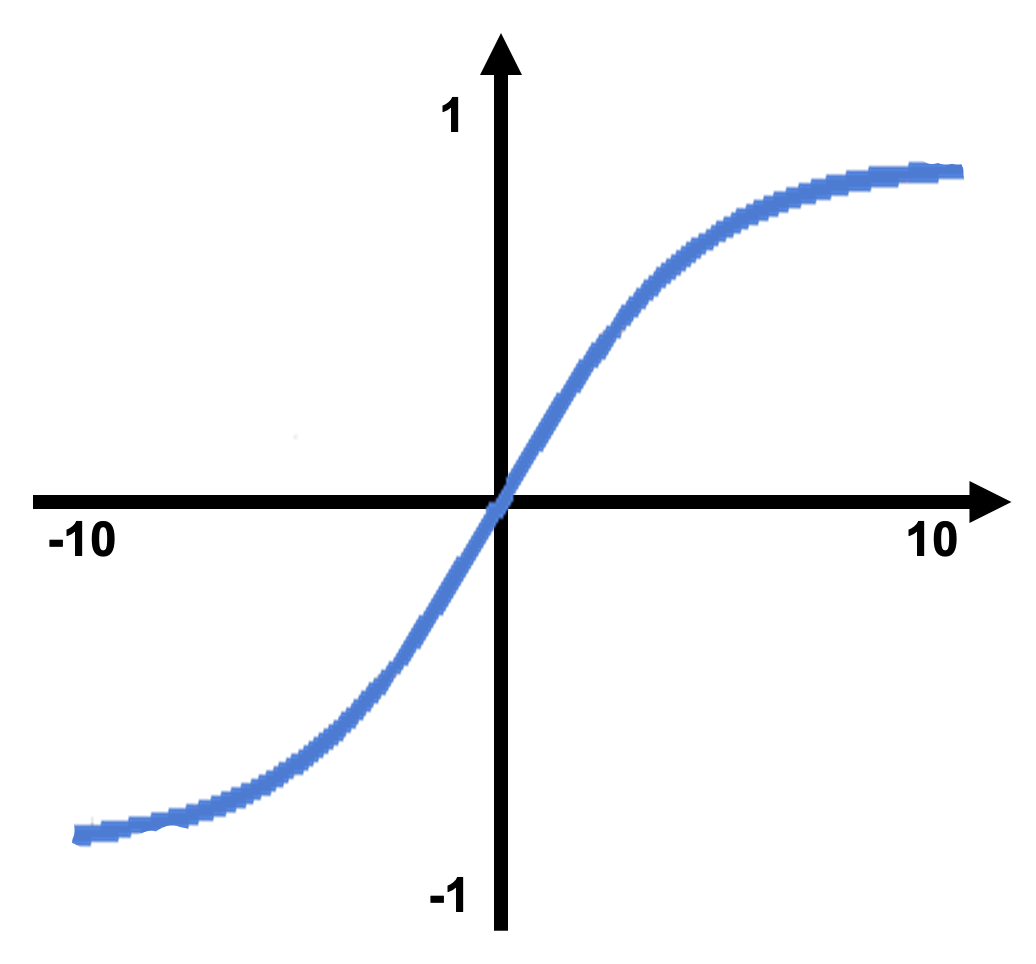
\includegraphics[width=0.3\textwidth]{ figures/estadoarte/tanh.png}}
	        \hspace{10pt}
	        \subfigure[]{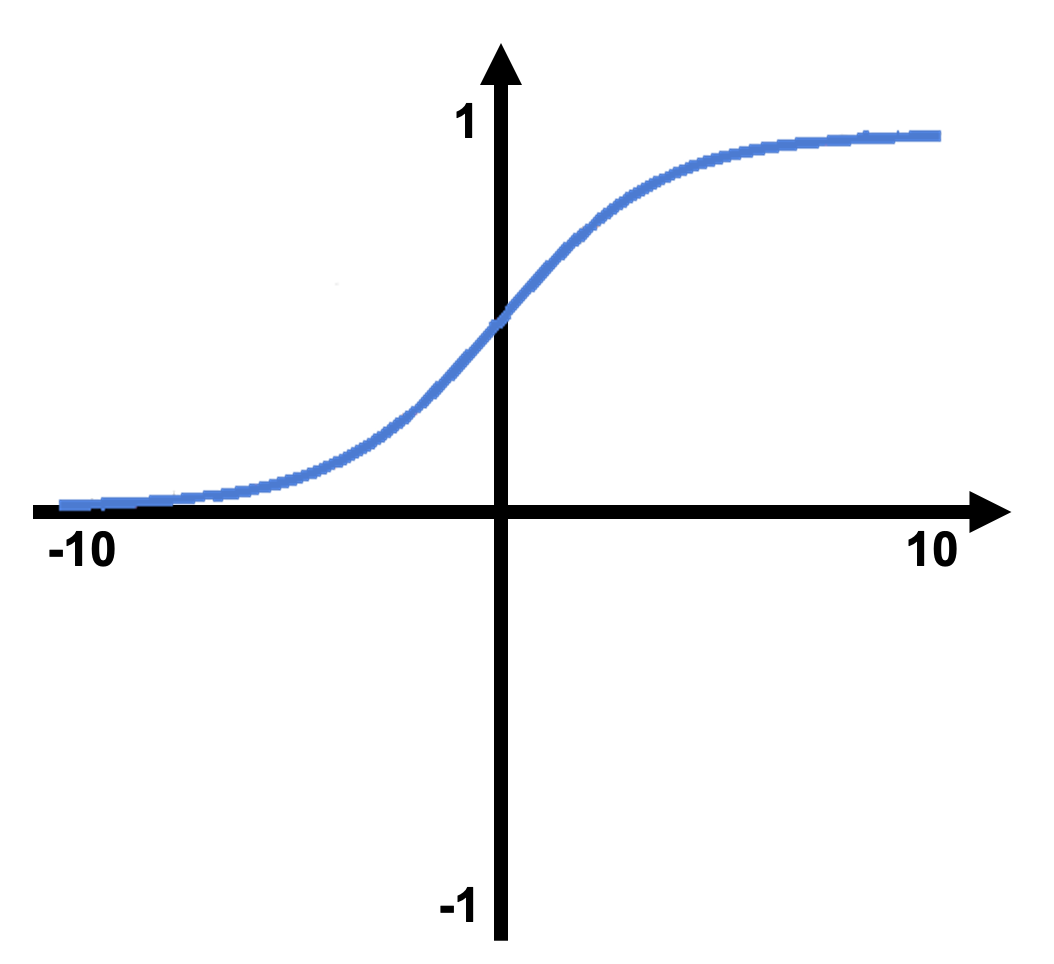
\includegraphics[width=0.3\textwidth]{ figures/estadoarte/softmax.png}}
	        \caption{Funciones de activación: (a)~Lineal, (b)~ReLu, (c)~Tanh y (d)~Softmax.}
			\label{fig.activacion}
		\end{center}
\end{figure}
\vspace{-10pt}

\subsection{Servidor Tamino}
Para la ejecución de los distintos procesos de este trabajo se ha utilizado un servidor Linux, Tamino, que está situado en el CPD de la ETSIT-URJC y pertenece a \textit{RoboticsLabURJC}. Las principales características de este servidor son:

\begin{itemize}
    \item \textbf{Procesador:} Intel(R) Xeon(R) CPU E5-2609 v4 @ 1.70GHz.
    \item \textbf{Número de núcleos:} 8 cores.
    \item \textbf{Memoria RAM:} 64GB.
    \item \textbf{GPU:} GeForce GTX 1080.
\end{itemize}

El uso de esta máquina ha permitido realizar entrenamientos más potentes así como el uso de conjuntos de datos más grandes.
\lhead[]{CAPÍTULO \thechapter. GENERACIÓN DE SECUENCIAS DE VÍDEO SINTÉTICAS}
\chapter{Generación de secuencias de vídeo sintéticas}\label{cap.generacion}

En este trabajo se va a evaluar el poder de predicción de distintas redes neuronales profundas. La exploración en este ámbito se realizará de forma progresiva: primero con píxeles que se mueven linealmente, posteriormente con otros que se mueven parabólicamente y finalmente otros que se mueven siguiendo una función sinusoidal. Es decir, se modifican las dinámicas de movimiento con una complejidad creciente. Para entrenar estas redes neuronales es necesario tener un conjunto grande de imágenes "etiquetas" con las que aprender a predecir. Se ha programado una aplicación que genera automáticamente esos conjuntos voluminosos siguiendo esas dinámicas con sus parámetros correspondientes, a la vez que divide el conjunto en los subconjuntos de entrenamiento, validación y \textit{test}. En la Figura~\ref{fig.gen_cajanegra} se presenta un diagrama ``caja negra'' del funcionamiento de dicha aplicación, en la que se parte de un fichero de configuración y se obtiene una base de datos con las muestras deseadas.

\begin{figure}[H]
		\begin{center}
			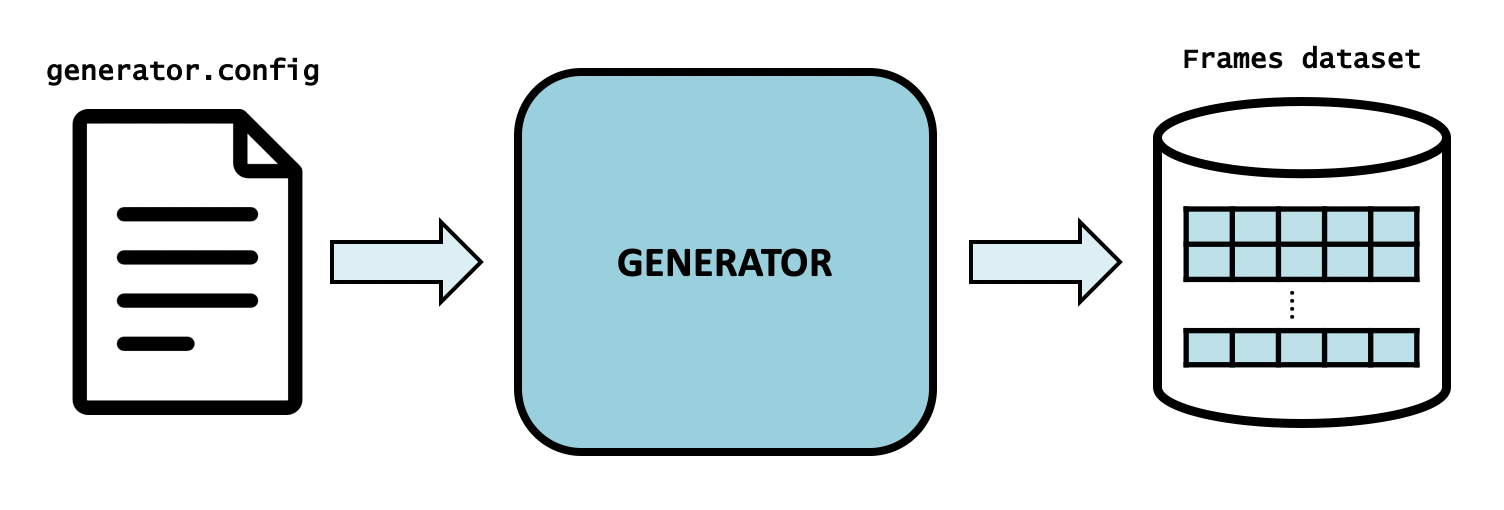
\includegraphics[width=0.8\textwidth]{ figures/generador.png}
			\caption{Diagrama ``caja negra'' del generador.}
			\label{fig.gen_cajanegra}
		\end{center}
\end{figure}

En este capítulo se explican los dos tipos de imágenes que se han considerado, modeladas y crudas, y se exponen las distintas dinámicas de movimiento entre fotogramas que se aplican dentro de un mismo subconjunto. Así mismo, se expondrá el código desarrollado para la generación de los conjuntos de datos que se utilizarán para entrenar las redes neuronales profundas de predicción y para validar experimentalmente la calidad sus predicciones, el nivel de acierto.


\section{Propiedades del \textit{dataset}}

Esta sección hace hincapié en las características de los \textit{datasets} generados con secuencias de vídeo. Se explica en profundidad la estructura que tiene el directorio que almacena los distintos conjuntos utilizados, los dos tipos de imágenes considerados, modeladas y crudas, y las tres dinámicas que han sido estudiadas, lineal, parabólica y sinusoidal.\\

Un \textit{dataset} generado se corresponde con una base de datos en la que se almacenan \textit{n}\_\textit{samples} muestras, cada una de las cuales es una colección de \textit{n}\_\textit{points}$+1$ fotogramas. En la Figura~\ref{fig.dataset} se muestra un esquema general del aspecto que presenta un conjunto de datos utilizado en este trabajo.

\begin{figure}[H]
		\begin{center}
			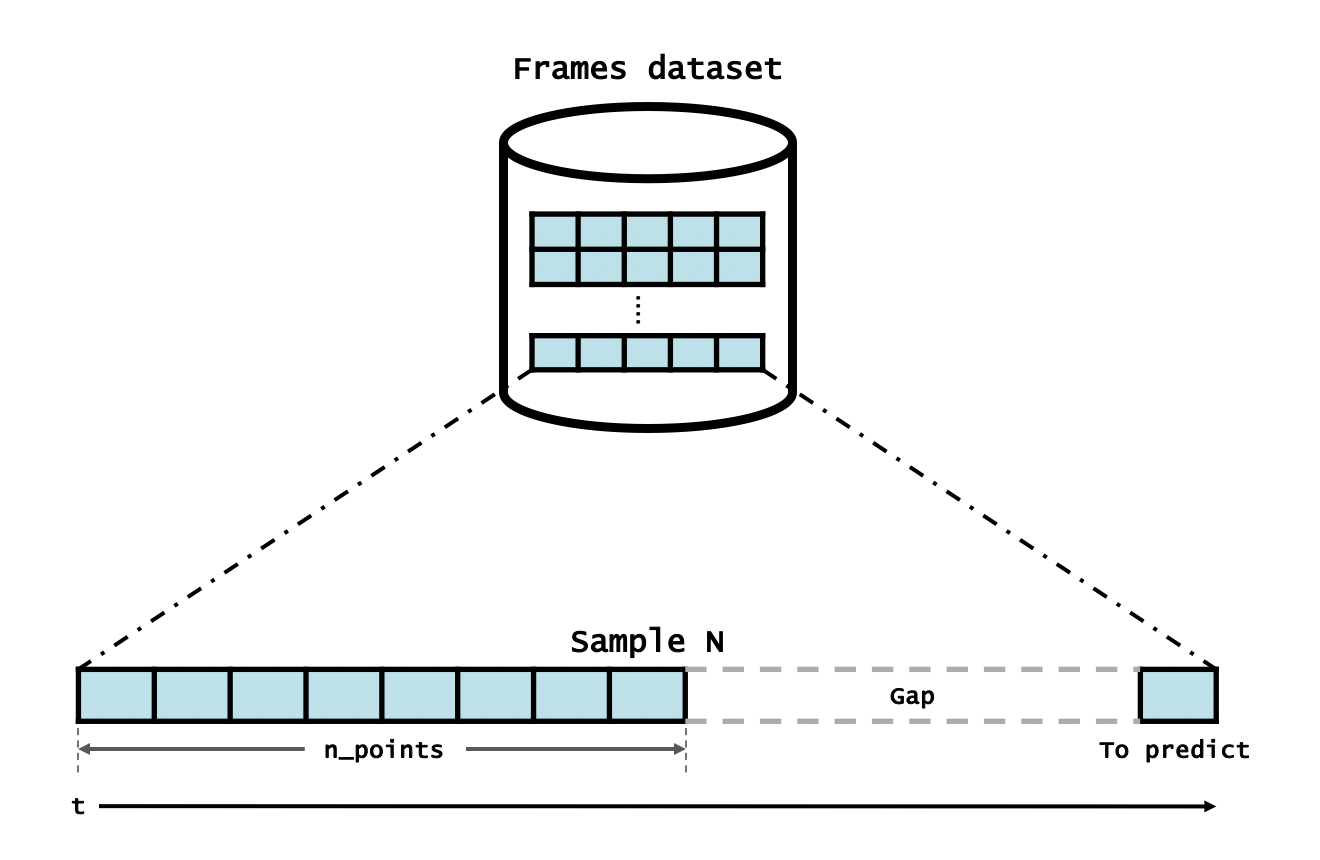
\includegraphics[width=0.85\textwidth]{ figures/dataset.png}
			\caption{Vista general de un \textit{dataset}.}
			\label{fig.dataset}
		\end{center}
\end{figure}

\subsection{Estructura del \textit{dataset}} \label{ap.estructura}

En la Figura~\ref{fig.estructura_dataset} se presenta un esquema de la estructura resultante con la ejecución del código explicado en la Sección~\ref{sec.generador} para diferentes parámetros~(de 1 a n). 
\vspace{5pt}
\begin{figure}[H]
	\begin{center}
	    \setlength{\fboxsep}{0.5cm}
	    \fbox{
        \begin{minipage}{6.7cm}
          \dirtree{%
          .1 Frames dataset.
          .2 Specific parameters \textit{1}.
          .3 Train.
          .4 Modeled samples.
          .5 \textit{sample0.txt}.
          .5 \vdots.
          .4 Raw samples.
          .5 sample0.
          .6 \textit{0.png}.
          .6 \vdots.
          .5 \vdots.
          .4 \textit{parameters.txt}.
          .3 Test.
          .4 \vdots.
          .3 Val.
          .4 \vdots.
          .2 \vdots.
          .2 Specific parameters \textit{n}.
          }
        \end{minipage}
        }
	    \caption{Estructura creada para el almacenamiento del \textit{dataset}.}
	    \label{fig.estructura_dataset}
	\end{center}
\end{figure}
\vspace{-10pt}
En el primer nivel de esta estructura, \textit{Frames dataset}, se distingue entre los distintos tipos de datos que se pueden generar. A pesar de que en este trabajo se ha centrado en las secuencias de imágenes, el generador fue diseñado para poder obtener otros dos tipos de datos: funciones y vectores, que tendrían su directorio homólogo en este mismo nivel.\\

En el segundo nivel se hace una distinción en función de los parámetros concretos que se hayan establecido en el fichero de configuración, explicado en el Apartado~\ref{ap.fichero}. Estos valores son:

\begin{itemize}
    \setlength\itemsep{1pt}
    \item Tipo de dinámica.
    \item Forma y color del objeto.
    \item Grados de libertad.
    \item Número de muestras.
    \item Tamaño de la imagen.
\end{itemize}

Dentro de cada uno de estos directorios se presenta siempre la misma estructura. La primera división existente es la de los subconjuntos de entrenamiento, \textit{test} y validación. Si no se hubiese indicado la realización de esta división, este nivel sería obviado y se pasaría directamente al siguiente. Todas estas carpetas presentan a su vez la misma estructura, sobre la que la herramienta de generación escribe directamente las distintas muestras: el fichero de parámetros, la carpeta con las muestras modeladas y la correspondiente a las muestras en crudo.

\subsection{Tipos de imágenes} \label{ap.tip_img}

Se han considerado dos tipos de imágenes para los distintos estudios sobre predicción visual que se han desarrollado en el trabajo. Ambos tipos de imágenes tienen una correspondencia entre sí, es decir, para una misma muestra se presenta la misma información en dos formatos distintos: valores numéricos e imágenes puras de píxeles.
En cuanto al contenido, todas las imágenes constan de un fondo negro y un único punto de luz móvil blanco, un píxel iluminado, que se desplaza dentro del fotograma siguiendo cierta dinámica.

\subsubsection{Imágenes modeladas}

Las datos modelados son una forma simplificada de mostrar las distintas posiciones que adquiere el píxel móvil en cada instante de tiempo. Con este tipo de imágenes se consigue representar la misma información de una forma compacta, se utiliza un total de \textit{$2 * n\_points$}  valores de entrada a la red, y \textit{$2$} valores de salida de la misma, reduciendo considerablemente la complejidad de las distintas redes que se estudien. En la Tabla~\ref{tab.modelada} se presenta un ejemplo concreto de cómo se representan estas muestras.

\begin{table}[H]
	\centering
	\begin{tabular}{{l|c|c|}}
		\hline
		\multicolumn{1}{|l|}{\textbf{\textit{t}}} & \textbf{\textit{x}} & \textbf{\textit{y}}\\\hline 
		\multicolumn{1}{|l|}{\textbf{0}} & 0 & 40\\ \hline
		\multicolumn{1}{|l|}{\textbf{1}} & 3 & 38\\ \hline
		\multicolumn{1}{|l|}{\textbf{2}} & 6 & 37\\ \hline
		\multicolumn{1}{|l|}{\textbf{3}} & 9 & 36\\ \hline
		\multicolumn{1}{|l|}{\textbf{\vdots}} & \vdots & \vdots\\ \hline
		\multicolumn{1}{|l|}{\textbf{29}} & 87 & 4\\ \hline
		
	\end{tabular}
	\caption{Ejemplo de imagen modelada.}
	\label{tab.modelada}
\end{table}

Estos datos se almacenan en la carpeta \textit{modeled}\_\textit{samples} mediante un fichero \textit{"sample[n].txt}, donde \textit{n} hace referencia al número del ejemplo durante su creación. Este fichero presenta una cabecera y un número de filas que se corresponde al número de instantes conocidos más el instante que se quiere predecir. La información viene distribuida en dos columnas, correspondientes con los valores \textit{x} e \textit{y} del píxel en cada instante de tiempo, que no se representa de forma explícita sino que se asocia con el orden de las filas.

\subsubsection{Imágenes crudas}

Las imágenes crudas son las imágenes propiamente dichas. En la Figura~\ref{fig.cruda} se muestra una composición donde se superponen todas las imágenes que forman la secuencia agrupadas en una única imagen.

\begin{figure}[H]
		\begin{center}
			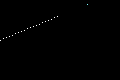
\includegraphics[width=0.6\textwidth]{ figures/samples/linear_sample.png}
			\caption{Ejemplo de muestra cruda.}
			\label{fig.cruda}
		\end{center}
\end{figure}
\vspace{-10pt}
Cada uno de las fotogramas presentaría un único píxel activo que se corresponde con el objeto del que se simula el movimiento y se almacena con el nombre \textit{"[n].png"} en la carpeta \textit{"sample[m]"}, donde \textit{"n"} sería el orden del instante de tiempo y \textit{"m"} el de la muestra generada. Cada una de estas carpetas que identifica una muestra es almacenada en el directorio \textit{raw}\_\textit{samples} que confluye todos los ejemplos del mismo tipo.\\

En este caso, a pesar de que la información es la misma, la cantidad de valores que se utilizan para representarla es mucho mayor. Se utiliza un total de \textit{$h * w * n\_points$}  valores de entrada a la red, y \textit{$h * w$} valores de salida de la misma, complicando las redes a estudiar.

\subsection{Tipos de dinámicas} \label{ap.dinamicas}

El movimiento del píxel en el vídeo viene determinado por tres dinámicas distintas, que van aumentando el grado de complejidad del mismo y ponen a prueba la capacidad de predicción de las redes. Además de las tres dinámicas que se han considerado: lineal, parabólica y  sinusoidal, dentro de cada una de ellas se aumenta de forma escalonada la dificultad incrementando el número de variables que adquieren un valor aleatorio, es decir, los \acrfull{dof} de las mismas.\\

Estas dinámicas afectan únicamente a la posición \textit{y} del píxel, y se utilizan los valores de \textit{x} obtenidos mediante la aplicación de un \acrfull{urm} al instante de tiempo con una velocidad aleatoria.

\subsubsection{Dinámica lineal}

La primera dinámica, y la más sencilla de todas, simula el movimiento del objeto en una línea recta a distintas velocidades y con distintas pendientes. Este movimiento se puede asimilar con el movimiento de un vehículo con una velocidad constante, sin tener en cuenta los efectos del rozamiento por la superficie ni la perspectiva. Para ello, utiliza la ecuación de la recta:
$$y = m*x + y0$$
que se materializa en el código de la siguiente forma:
\vspace{10pt}
\begin{lstlisting}[frame=single]
  self.g = lambda x, y0, m: (m * x) + y0
\end{lstlisting}

En la Figura~\ref{fig.lineal} se presenta un ejemplo de esta dinámica con todas las imágenes que lo conforman superpuestas en una sola.

\begin{figure}[H]
		\begin{center}
			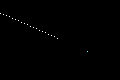
\includegraphics[width=0.6\textwidth]{ figures/samples/linear2_sample.png}
			\caption{Ejemplo de dinámica lineal.}
			\label{fig.lineal}
		\end{center}
\end{figure}
\vspace{-10pt}
Por la propia naturaleza de la ecuación, es posible ir modificando la complejidad del movimiento a medida que incrementamos la cantidad de parámetros que se asignan de forma aleatoria, es decir, los \acrshort{dof}. A continuación, se exponen los distintos casos que se dan en la dinámica actual.

\begin{description}
\item[Pendiente nula] \hfill 
\vspace{10pt}
\\
El movimiento más sencillo que se puede encontrar es un caso especial de la dinámica lineal. Ocurre cuando se fija la pendiente de la recta (\textit{m}) en un valor nulo, igualando el valor de la posición a una altura inicial. De esta forma se obtiene la ecuación simplificada:
$$y = y0$$
que se presenta en el código de la siguiente manera:
\vspace{10pt}
\begin{lstlisting}[frame=single]
  self.g = lambda x, y0: y0
\end{lstlisting}
La altura inicial se puede asignar de dos maneras distintas::
\vspace{10pt}
\begin{lstlisting}[frame=single]
  y0 = int(self.h / 2) #1
  y0 = random.randint(1, self.h - 1) #2
\end{lstlisting}
La primera línea asigna la altura a la mitad de la imagen (\textit{h/2}), mientras que con la segunda se establece un valor aleatorio entre los límites de la imagen, que introduce un nuevo \acrshort{dof}.

En la Figura~\ref{fig.urm} se muestra un ejemplo de este caso especial de la dinámica lineal.
\begin{figure}[H]
		\begin{center}
			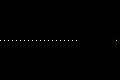
\includegraphics[width=0.6\textwidth]{ figures/samples/URM_sample.png}
			\caption{Ejemplo del caso con pendiente nula.}
			\label{fig.urm}
		\end{center}
\end{figure}

\item[\textbf{1 \acrshort{dof}}] \hfill 
\vspace{10pt}
\\
El primer parámetro de la ecuación que toma un valor aleatorio en cada muestra es la pendiente de la recta, dejando fija la altura inicial del punto. El código que se utiliza en cada iteración para la definición de los parámetros es el siguiente:
\vspace{10pt}
\begin{lstlisting}[frame=single]
  m = np.round(random.uniform(-self.h/10, self.h/10), 2)
  y0 = int(self.h / 2)
\end{lstlisting}
Los límites que se establecen para obtener el valor aleatorio son orientativos. Pretenden reducir al máximo el intervalo que asegure la presencia del punto en todas las imágenes pero esta presencia no llega a asegurarse en su totalidad. Es por esto que, posteriormente, se realiza una comprobación de las posiciones obtenidas.
\vspace{90pt}
	
\item[\textbf{2 \acrshort{dof}}] \hfill 
\vspace{10pt}
\\
Se deja que todos los parámetros de la ecuación tomen un valor aleatorio distinto en cada muestra, tanto la pendiente como la altura inicial. Para esta asignación se implementa el siguiente código:
\vspace{10pt}
\begin{lstlisting}[frame=single]
  m = np.round(random.uniform(-self.h/10, self.h/10), 2)
  y0 = random.randint(1, self.h - 1)
\end{lstlisting}
Al igual que en el caso anterior, los límites establecidos son orientativos para cumplir con las limitaciones del \textit{dataset}.
\vspace{10pt}

\end{description}

\subsubsection{Dinámica parabólica}

La dinámica parabólica, que aumenta el grado de complejidad mediante el incremento del número de parámetros necesarios para su definición, utiliza la ecuación de la parábola para obtener las posiciones \textit{y}:
$$y = a*t^2 + b*t + c$$
que se implementa en el código de mediante las siguiente línea:
\vspace{10pt}
\begin{lstlisting}[frame=single]
  self.g = lambda x, a, b, c: a * (x ** 2) + b * x + c
\end{lstlisting}

En la Figura~\ref{fig.parab} se puede ver un ejemplo, con el mismo formato que el de la dinámica anterior, de este tipo de movimiento.

\begin{figure}[H]
		\begin{center}
			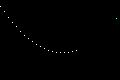
\includegraphics[width=0.6\textwidth]{ figures/samples/parabolic_sample.png}
			\caption{Ejemplo de dinámica parabólica.}
			\label{fig.parab}
		\end{center}
\end{figure}
\vspace{-10pt}

Al igual que en el caso lineal, se va incrementando la complejidad de la dinámica  aumentando el número de \acrshort{dof}, explicados a continuación.

\begin{description}
\item[\textbf{1 \acrshort{dof}}] \hfill 
\vspace{10pt}
\\
El parámetro que se modifica en este primer caso es el que acompaña al término cuadrático (\textit{a}), de tal forma que la definición de los parámetros queda de la siguiente manera: 
\vspace{10pt}
\begin{lstlisting}[frame=single]
  a = round(random.uniform(-0.75, 0.75), 3)
  b = 1.5
  c = int(self.h / 2)
\end{lstlisting}
El valor otorgado a \textit{b} deriva de una serie de pruebas para obtener aquel que mejor se ajustase a lo que se buscaba mientras que la altura inicial (\textit{c}) se establece en la mitad de la imagen. Por otro lado, al igual que ocurre en la dinámica lineal, los límites escogidos de la muestra son orientativos para cumplir con la presencia del píxel en todas las imágenes, pero en ningún caso la asegura. 
\vspace{10pt}
\item[\textbf{2 \acrshort{dof}}] \hfill 
\vspace{10pt}
\\
El siguiente parámetro a modificar es la altura inicial, que en este caso se establece con el parámetro \textit{c}. Siguiendo la definición del caso lineal,los parámetros de este caso quedan definidos de la siguiente manera:
\vspace{10pt}
\begin{lstlisting}[frame=single]
  a = round(random.uniform(-0.75, 0.75), 3)
  b = 1.5
  c = random.randint(1, self.h - 1)
\end{lstlisting}
\vspace{10pt}

\item[\textbf{3 \acrshort{dof}}] \hfill 
\vspace{10pt}
\\
En el último caso se definen todos los parámetros de la ecuación mediante un valor aleatorio. Con esta premisa, la definición de los parámetros presenta la siguiente forma:
\vspace{40pt}
\begin{lstlisting}[frame=single]
  a = round(random.uniform(-0.75, 0.75), 3)
  b = round(random.uniform(-2, 2), 3)
  c = random.randint(1, self.h - 1)
\end{lstlisting}
\vspace{10pt}

\end{description}

\subsubsection{Dinámica sinusoidal}
La dinámica más compleja considerada en este trabajo, la sinusoidal, hace uso de la función trigonométrica del seno para el cálculo de posiciones en el eje vertical. Su expresión es la siguiente:
$$y = a*sin(2*\pi*f*x + b) + c$$
y se traduce en el código en la línea:
\vspace{10pt}
\begin{lstlisting}[frame=single]
  self.g = lambda x, a, b, c, f: 
    a * math.sin(2 * math.pi * f * math.radians(x) + b) + c
\end{lstlisting}

En la Figura~\ref{fig.sin} se muestra un ejemplo de la dinámica mediante la superposición de las imágenes en una sola.

\begin{figure}[H]
		\begin{center}
			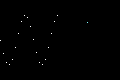
\includegraphics[width=0.6\textwidth]{ figures/samples/sinusoidal_sample.png}
			\caption{Ejemplo de dinámica sinusoidal.}
			\label{fig.sin}
		\end{center}
\end{figure}
\vspace{-10pt}
De la misma forma que sucede con las otras dos dinámicas, se aumenta la dificultad del movimiento mediante el aumento  de los \acrshort{dof}, que se exponen a continuación.
\vspace{150pt}
\begin{description}
\item[\textbf{1 \acrshort{dof}}] \hfill 
\vspace{10pt}
\\
El primer parámetro que se establece de forma aleatoria es la frecuencia (\textit{f}) del seno. La definición de los parámetros para este caso queda de la siguiente manera:
\vspace{10pt}
\begin{lstlisting}[frame=single]
  a = 25
  f = round(random.uniform(0.5, 5), 2)
  b = 0
  c = int(self.h / 2)
\end{lstlisting}

Como ocurre en el caso parabólico, los valores de los parámetros fijados se han obtenido mediante distintas pruebas con el objetivo de que sean lo más adecuados para los estudios realizados. De igual forma, los límites establecidos son orientativos para cumplir con las limitaciones del \textit{dataset}.
\vspace{10pt}
	
\item[\textbf{2 \acrshort{dof}}] \hfill
\vspace{10pt}
\\
El segundo parámetro que se deja libre es, de nuevo, la altura inicial de la imagen en la que comienza el movimiento, dando lugar a la siguiente definición de parámetros:
\begin{lstlisting}[frame=single]
  a = 25
  f = round(random.uniform(0.5, 5), 2)
  b = 0
  c = random.randint(1, self.h - 1)
\end{lstlisting}

\item[\textbf{3 \acrshort{dof}}] \hfill 
\vspace{10pt}
\\
El tercer parámetro que obtiene valores aleatorios en esta dinámica es la amplitud del seno, y se definen los parámetros de este caso con el siguiente código:
\vspace{10pt}
\begin{lstlisting}[frame=single]
  a = random.randint(15, 40)
  f = round(random.uniform(0.5, 5), 2)
  b = 0
  c = random.randint(1, self.h - 1)
\end{lstlisting}
\vspace{50pt}
\item[\textbf{4 \acrshort{dof}}] \hfill 
\vspace{10pt}
\\
Por último se permite que todos los parámetros tomen valores aleatorios, dando lugar al caso más complejo de este movimiento. Para ello se usa el siguiente código:
\vspace{10pt}
\begin{lstlisting}[frame=single]
  a = random.randint(15, 40)
  f = round(random.uniform(0.5, 5), 2)
  b = round(random.uniform(0, 2 * math.pi), 3)
  c = random.randint(1, self.h - 1)
\end{lstlisting}
\vspace{10pt}
\end{description}
\section{Herramienta de generación} \label{sec.generador}

Para la elaboración propia de los distintos conjuntos de datos,  se ha desarrollado un código\footnote{\url{https://github.com/RoboticsLabURJC/2017-tfm-nuria-oyaga/tree/master/Generator}} en Python que, a través de la fijación de varios parámetros en un fichero de configuración, elabora un conjunto de muestras que se adapta al estudio concreto en el que se vaya a aplicar. En esta sección se explican las dos partes fundamentales de este código: la especificación de los parámetros y la propia generación y almacenamiento de las muestras.

\subsection{Fichero de configuración} \label{ap.fichero}

A través de este fichero se establecen los parámetros principales que definen las características del \textit{dataset} a generar. A continuación se explican los distintos valores a definir y lo que supone modificar cada uno de ellos. 

\begin{basedescript}{\desclabelstyle{\pushlabel}\desclabelwidth{2.75cm}}
\item[\textit{root}] Define la ruta en la que se almacenará la estructura de carpetas y archivos que se genera en la ejecución del código.
\item[\textit{to\_generate}] Indica el tipo de dato que va a ser generado. A pesar de que este proyecto se centra en el estudio con imágenes, el generador se desarrolló con la posibilidad de generar datos de tres tipos: funciones, vectores unidimensionales e imágenes.
\item[\textit{motion\_type}] Especifica el tipo de movimiento, la dinámica que sigue el objeto entre cada \textit{frame}, explicadas en el apartado~\ref{ap.dinamicas}.
\item[\textit{height}]  Número entero que indica la altura de la imagen, su dimensión \textit{y}. En este trabajo se utiliza una altura de 80 píxeles.
\item[\textit{width}]  Número entero que indica el ancho de la imagen, su dimensión \textit{x}. En este trabajo se utiliza un ancho de 120 píxeles.
\item[\textit{object}]  Define el tipo de objeto que se mueve en la imagen. En este trabajo únicamente se utiliza el objeto píxel, de tal forma que toda la imagen será negra a excepción de un punto activo que será considerado el objeto.
\item[\textit{obj\_color}]  Permite definir el color del objeto. Se utiliza un único nivel de intensidad en el caso del píxel y una terna RGB para otros objetos.
\item[\textit{dof}] Establece los grados de libertad de la dinámica de movimiento, es decir, el número de variables que se generan de forma aleatoria en la ecuación que la define.
\item[\textit{n\_samples}]  Número entero que indica el número de muestras totales que se generarán en el conjunto.
\item[\textit{n\_points}] Número entero que indica la cantidad de instantes de tiempo que serán utilizados para predecir.
\item[\textit{gap}] Número entero que define la separación temporal, instantes de tiempo, entre la última muestra conocida y la muestra a predecir.
\item[\textit{noise}] Permite añadir ruido de un determinado tipo a las muestras para un estudio más avanzado.
\item[\textit{split}] Indica si se dividirá el conjunto en los tres subconjuntos (\textit{train}, \textit{validation}, \textit{test}) y la proporción en la que lo hará si así de define.
\end{basedescript}

De esta manera, se permite un ajuste más sencillo del \textit{dataset} a generar al tipo de problema que se quiera estudiar, dejando al gusto del usuario las características del mismo.
    
\subsection{Generación del \textit{dataset}} \label{ap.generacion}

En la Figura~\ref{fig.flujo_gen} se expone el diagrama del flujo que sigue el programa encargado de la generación del \textit{dataset}, centrándose en el tipo de dato que es de interés en este trabajo: los fotogramas.\\
\vspace{10pt}
\begin{figure}[H]
    \begin{center}
        \begin{tikzpicture}[node distance=2.5cm]
            \node (cd) [treenode] {Creación de \\ directorios};
            \node (def) [treenode, below of=cd] {Definición de muestra};
            \node (obt) [treenode, below of=def] {Obtención de muestra};
            \node (val) [decision, below of=obt, yshift=-0.25cm] {¿Es válida?};
            \node (gen) [treenode, below of=val, yshift=-0.25cm] {Generación de imágenes};
            \node (div) [decision, below of=gen, yshift=-0.25cm] {¿División?};
            \node (asig) [treenode, below of=div, yshift=-0.25cm] {Asignación de subconjunto};
            \node (sav) [treenode, right of=div, xshift=3cm] {Almacenamiento de muestras};
            
            \draw [arrow] (cd) -- (def);
            \draw [arrow] (def) -- (obt);
            \draw [arrow] (obt) -- (val);
            \draw [arrow] (val) -- node[anchor=east, yshift=0.3cm] {Sí} (gen);
            \draw [arrow] (val) --  node[anchor=south, xshift=-0.35cm] {No} ++ (3cm,0cm) |-(obt);
            \draw [arrow] (gen) -- (div);
            \draw [arrow] (div) -- node[anchor=east, yshift=0.3cm] {Sí} (asig);
            \draw [arrow] (div) --  node[anchor=south, xshift=-0.6cm] {No} (sav);
            \draw [arrow] (asig) -- ++ (5.5cm,0cm) |- (sav.south);
            \draw [arrow] (sav) |- node[align=center, anchor=west, yshift=-5cm, xshift=0.2cm] {\textit{for n in}\\ \textit{n}\_\textit{samples}} (def);
        \end{tikzpicture}
        \caption{Diagrama de flujo del generador.}
	    \label{fig.flujo_gen}
	\end{center}
\end{figure}
\vspace{-10pt}
En primer lugar se comprueban y se crean, en caso de ser necesario, los directorios que son necesarios para el almacenamiento del conjunto según la ruta que ha sido indicada en el fichero de configuración. La estructura de ficheros que se crea con el fin de almacenar todas las muestras del conjunto es explicada en el apartado~\ref{ap.estructura}.\\

Tras la creación de la estructura necesaria se entra en un bucle, que se itera el número de muestras que haya sido definido, en el que se define, obtiene, valida, genera y almacena cada uno de los ejemplos que conforman el \textit{dataset}.\\

Para la definición de la muestra se utiliza la clase correspondiente al tipo de movimiento que se vaya a implementar, la cual tiene definida de forma interna la ecuación que se corresponde con la dinámica. Este tipo de dinámica a implementar viene indicada en el fichero de configuración y todas las clases y ecuaciones que son utilizadas se explican en profundidad en el Apartado~\ref{ap.dinamicas}.\\

Tras definir la muestra se llama a la función encargada de generarla. A grandes rasgos, esta función obtiene las posiciones \textit{(x,y)} del píxel en cada uno de los fotogramas y comprueba que esta posición obtenida no se salga de los límites de la imagen, evitando así oclusiones y desapariciones. Para obtener esas posiciones se realizan varios pasos que, aunque pueden variar en número en función de la dinámica y de los grados de libertad, siguen siempre la misma estructura. Esta estructura queda encapsulada en un bucle \textit{while}, que será detenido una vez se obtenga un conjunto de posiciones válidas, con las siguientes operaciones:

\begin{enumerate}
  \item Se define el movimiento que sigue el píxel en el eje \textit{x}, identificado con el instante temporal \textit{t} y, por tanto, con la velocidad a la que se mueve el píxel. Éste es el mismo independientemente de la dinámica con la que se esté trabajando, se corresponde con un \acrshort{urm} y viene definido de la siguiente forma:
  \vspace{10pt}
  \begin{lstlisting}[frame=single]
  self.f = lambda t, x0, u_x: x0 + u_x * t
  \end{lstlisting}
  Para poder definir el movimiento \acrshort{urm} en los conjuntos desarrollados se fija el punto de inicio (\textit{x0}) en el instante 0 y se asigna una velocidad aleatoria para cada una de las muestras. Esta asignación se realiza mediante el siguiente código:
  \vspace{10pt}
  \begin{lstlisting}[frame=single]
  limit = int(self.w / (self.n_points + self.gap))
  u_x = random.randint(1, limit)
  \end{lstlisting}
  Así se establece un límite en la velocidad, en función del número de instantes de tiempo conocidos y la separación entre el instante a predecir y el último conocido, que asegura la aparición del píxel en todas las imágenes de la muestra.
  
  \item Se obtienen los valores concretos de la posición \textit{x} en cada instante de tiempo de la siguiente forma:
  \vspace{10pt}
  \begin{lstlisting}[frame=single]
  numbers_x = [self.f(x, x0, u_x) for x in range(self.n_points)]
  numbers_x.append(self.f(self.n_points + self.gap - 1, x0, u_x))
  \end{lstlisting}
  Primero se calculan todos los valores de los instantes de tiempo conocidos (\textit{n}\_\textit{points}) y, posteriormente, se añade el valor correspondiente con el instante a predecir (\textit{n}\_\textit{points+gap}).
  
  \item Se define el valor de todas las variables que son necesarias para aplicar la ecuación de la dinámica y obtener las posiciones en el eje \textit{y}. La forma de definir estas variables, explicadas en el Apartado~\ref{ap.dinamicas}, dependen del grado de libertad que se haya indicado en el fichero de configuración. A medida que aumenta la complejidad aumenta el número de variables que se generan de forma aleatoria. 
  
  \item Se calculan las posiciones en el eje \textit{y}, en función de la dinámica que se haya establecido, mediante la siguiente línea:
  \vspace{10pt}
  \begin{lstlisting}[frame=single]
  numbers_y = [self.g(n_x, *args) for n_x in numbers_x]
  \end{lstlisting}
  Los argumentos que se pasan a la función de la dinámica serán las variables que previamente han sido definidas.
  
  \item Se comprueba que todas las posiciones se encuentren dentro de la imagen y, en caso positivo, se detiene el bucle y se continúa con el flujo del programa de generación. Si es negativo se repetirá el proceso hasta alcanzar un conjunto de posiciones válido.
\end{enumerate}

Una vez se han obtenido las posiciones del píxel válidas se procede a la generación de la propia secuencia de imágenes. Para ello se recorren todas las posiciones que han sido generadas (\textit{n}\_\textit{points} + 1) y se crea una imagen por cada una de ellas. La imagen se inicia con todos los píxeles nulos, completamente negra, y posteriormente se activa el píxel que se corresponde con la posición \textit{(y,x)} con el valor indicado en el fichero de configuración, para este proyecto fijado en 255. Se debe trasponer el vector de posición por la forma en la que Numpy establece el acceso a las posiciones en las imágenes\footnote{\url{https://scikit-image.org/docs/dev/user\_guide/numpy_images.html}}, primero las filas (\textit{y}) y luego a las columnas (\textit{x}).\\

Antes de almacenar la muestra, si se ha establecido la división del \textit{dataset} en los subconjuntos de entrenamiento, validación y \textit{test}, se asignará la misma al conjunto al que pertenece. Para esta asignación se utiliza un criterio de orden de la siguiente forma:

\begin{itemize}
    \setlength\itemsep{3pt}
    \item $n\_sample < n\_train \Rightarrow$ Conjunto de entrenamiento
    \item $n\_train \leqslant n\_sample < n\_train + n\_test\Rightarrow$ Conjunto de \textit{test}
    \item $n\_train + n\_test \leqslant n\_sample < n\_train + n\_test\ + n\_val \Rightarrow$ Conjunto de validación
\end{itemize}

Los valores que definen el número de muestras que tiene cada conjunto vienen dados por los distintos parámetros de división establecidos en el fichero de configuración. El código empleado para calcular estos valores es el siguiente:
\vspace{10pt}
\begin{lstlisting}[frame=single]
  n_test = int(n_samples * float(conf['split']['fraction_test']))
  n_val = int(n_samples * float(conf['split']['fraction_validation']))
  n_train = n_samples - n_val - n_test
\end{lstlisting}

En los conjuntos desarrollados para este trabajo, el \textit{flag} que indica la división estará siempre activado, pues se hace se hace uso de los tres subconjuntos diferenciados en las distintas fases de la investigación. Por lo tanto, el flujo del generador siempre será el mismo independientemente del tipo de dato que se esté generando, pasando la muestra por el proceso de asignación correspondiente.\\

Para el almacenamiento de la muestra en la carpeta correspondiente, la del subconjunto si se ha hecho división o la general en caso contrario, se realizan tres operaciones que permiten obtener información de la misma en distintos formatos.

\begin{itemize}
    \setlength\itemsep{3pt}
    \item \textbf{\textit{parameters.txt}}: Se escriben las distintas variables utilizadas para la generación de cada muestra. Cada fila de este fichero se corresponde con un ejemplo generado.
    \item \textbf{\textit{modeled}\_\textit{samples}}: Se guarda un fichero para cada muestra con las posiciones de la misma.
    \item \textbf{\textit{raw}\_\textit{samples}}: Se almacena una carpeta por muestra con las imágenes que la conforman.
\end{itemize}

Con todo esto se obtiene un directorio, cuya estructura se ha explicado más a fondo en el apartado~\ref{ap.estructura}, que contiene todo lo necesario para entrenar y evaluar las distintas redes que se estudian en el desarrollo de este proyecto.
\lhead[]{CAPÍTULO \thechapter. FIGURAS DE MÉRITO Y EVALUACIÓN}
\chapter{Figuras de mérito y evaluación}\label{cap.evaluacion}

Para evaluar de modo fiable la calidad de las redes neuronales profundas como predictores visuales se ha desarrollado una herramiento \textit{software} que obtienen unas figuras de mérito objetivas. El proceso de evaluación aplica las redes sobre los conjuntos de datos de test supervisados que se han descrito en el Capítulo~\ref{cap.generacion}, computa las figuras de mérito elegidas y las representa gráficamente para un mejor análisis. La comparación de estas gráficas de las distintas redes estudiadas es lo que permitirá extraer conclusiones sobre distintos parámetros.\\

En este capítulo se explican dichas figuras de mérito y se realiza un análisis en profundidad del código Python desarrollado para la evaluación, realizando también  una interpretación sobre los gráficos y resultados que arroja dicho código al terminar la ejecución.

\section{Figuras de mérito}

A continuación se describen las figuras de mérito que se han utilizado para evaluar las prestaciones de las redes, que se aplican tanto a imágenes modeladas como crudas. Para obtener conclusiones sobre la capacidad predictiva de las redes estudiadas se realiza una comparación entre dichas medidas. Estas comparaciones permiten obtener conclusiones sobre parámetros como el número de muestras utilizadas para entrenar, la complejidad de la dinámica o el horizonte temporal de predicción. Dichas conclusiones serán las que ayuden a tomar decisiones en la mejora del entrenamiento y la estructura de las redes para obtener la mejor red posible para la predicción.

\begin{description}
\item[Distancia entre píxeles] \hfill 
\vspace{10pt}
\\
La medida que se utiliza para cuantificar el error cometido en cada una de las predicciones es la distancia Euclídea\footnote{\url{https://en.wikipedia.org/wiki/Euclidean_distance}}  entre el píxel predicho~(\textit{p}) y el real~(\textit{q}). En dos dimensiones, su expresión viene dada por:  
$$d_E(p,q) = \sqrt{(p_1 - q_2)^2 + (p_1 - q_2)^2}$$

Además, para un  análisis más profundo, esta distancia se desglosa en cada una de las dimensiones de la imagen, \textit{x} e \textit{y}, simplemente calculando la diferencia en términos absolutos del valor en dichas coordenadas:
$$d_{E,dim}(p_{dim}, q_{dim}) = |p_{dim} - q_{dim}|$$

Las distancias anteriores cuantifican el error absoluto cometido en el plano de la imagen  y sus dimensiones \textit{x} e \textit{y}. Para analizar de una forma más completa la bondad de la red, se considera también el error relativo a la a la máxima distancia entre dos píxeles de la imagen, así como distintos estadísticos sobre las medidas de distancia.

\vspace{10pt}

\item[Distancia relativa] \hfill 
\vspace{10pt}
\\
La distancia absoluta puede dar una visión incompleta sobre el fallo que se ha cometido. Puesto que no es lo mismo desviarse una distancia de 5 píxeles en una imagen de 5x5 que en una de 1920x1080, se hace uso del error relativo\footnote{\url{https://en.wikipedia.org/wiki/Approximation_error}}. La medida relativa~($\eta$) normaliza la distancia absoluta~($\epsilon$) respecto a la máxima distancia en la imagen~($\upsilon$), haciendo uso de la siguiente fórmula:
$$\eta = \frac{\epsilon}{\upsilon}$$
En el caso de las imágenes, el máximo error a cometer es la mayor distancia entre dos píxeles de la imagen. Para una imagen de altura \textit{h} y anchura \textit{w}, la máxima distancia se corresponde con su diagonal, cuyo valor se obtiene de la siguiente manera:
$$\upsilon = \sqrt{h^2 + w^2}$$

La distancia relativa se suele indicar de forma porcentual, por lo que el valor calculado se multiplica por 100 para su expresión como porcentaje:
$$\delta = \eta * 100\%$$

La distancia relativa consigue normalizar la medida para una comparación más justa entre imágenes de distinto tamaño, permitiendo tener una idea más realista del fallo que se está cometiendo. 

\vspace{10pt}

\item[Estadísticos] \hfill 
\vspace{10pt}
\\
Para que la medición de la calidad de las predicciones sea fiable típicamente se aplica la red neuronal sobre un conjunto de secuencias, no sobre una única, es decir sobre varias secuencias supervisadas de fotogramas, que incluyen el fotograma verdadero en el tiempo de predicción. A partir de las medidas anteriores en dicho conjunto se obtienen una serie de estadísticos que permiten comparar las prestaciones de distintas redes y extraer conclusiones. A continuación se describen los estadísticos considerados.

\begin{itemize}
    \item \textbf{Máximo:} Se trata del error máximo cometido sobre todas las secuencias analizadas. Este valor identifica la imagen para la que más distancia existe entre la posición real y la predicha, que será uno de los elementos a tener en cuenta para examinar la bondad de la red. 
    \item \textbf{Media:} Se trata de la media de los vectores de error resultantes, absoluto y relativo, para obtener un único valor que permita hacer comparaciones rápidas.
\end{itemize}

\item[Formas de representación] \hfill 
\vspace{10pt}
\\
Para un mejor análisis de las figuras de mérito y los estadísticos presentados, se crean una serie de representaciones gráficas que contienen la información relevante para la comparación. Estas representaciones tienen su base en dos tipos:

\begin{itemize}
    \item \textbf{Histograma}\footnote{\url{https://en.wikipedia.org/wiki/Histogram}}: Se trata de un gráfico de barras que enfrenta la frecuencia con la que se comete un error con el valor del mismo, agrupado en intervalos para una representación más compacta.
    \item \textbf{\textit{Boxplot}}\footnote{\url{https://matplotlib.org/3.3.1/api/_as_gen/matplotlib.pyplot.boxplot.html}}: Se trata de un diagrama de caja y bigotes en el que la caja representa los cuartiles y las líneas que se extienden desde ella indican variabilidad fuera de los cuartiles superior e inferior. Por otro lado, los valores atípicos u \textit{outliers} se representan como puntos individuales dispersos por el eje vertical de la caja.
\end{itemize}

Todas las representaciones se combinan en una única figura, similar a la representada en la Figura~\ref{fig.test_example}, que se divide en cuatro regiones: una para el histograma del error absoluto, otra para el del relativo, una tercera para el \textit{boxplot} y la última con información de la media y el máximo. 

\begin{figure}[H]
		\begin{center}
			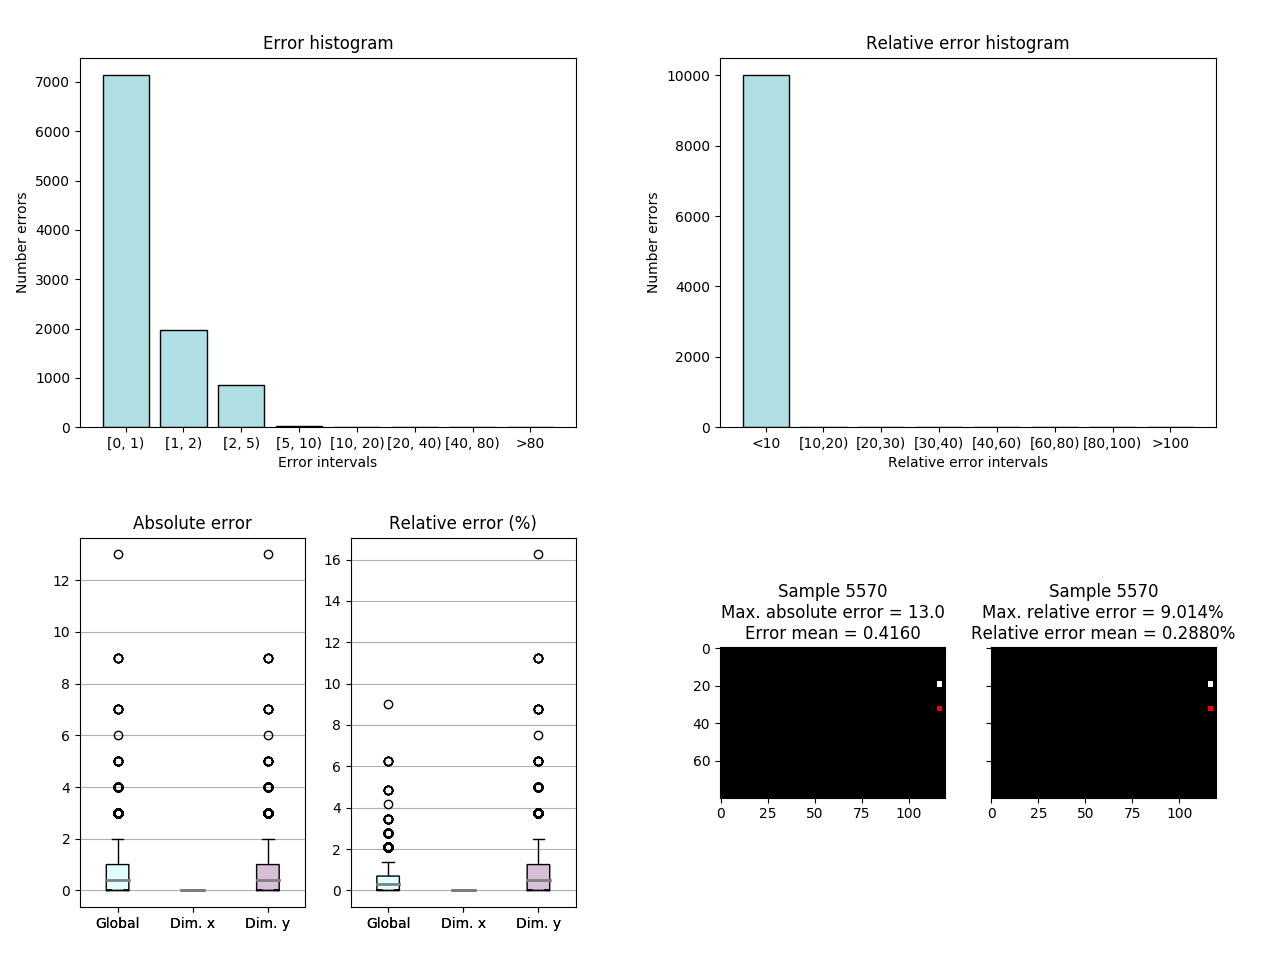
\includegraphics[width=0.9\textwidth]{ figures/error_stats_example.png}
			\caption{Ejemplo de gráfica con la distribución de distintas figuras de mérito y estadísticos asociados.}
			\label{fig.test_example}
		\end{center}
\end{figure}
\vspace{-10pt}

Con esta figura se representa de una forma resumida y clara toda la información referente las prestaciones de la red, a su calidad como predictor visual, facilitando la posterior tarea de análisis.
\vspace{10pt}
\end{description}

\section{Metodología de evaluación} \label{sec.eval}

Para el cálculo de las medidas  y la obtención de la Figura~\ref{fig.test_example} se ha desarrollado un código en Python sobre el que se profundiza en la siguiente sección.\\

En la Figura~\ref{fig.flujo_test} se muestra el flujo que sigue el código para evaluar una red concreta con un conjunto de \textit{test} determinado. El programa sigue un flujo muy sencillo y lineal cuyo resultado son la Figura~\ref{fig.test_example} y los valores asociados a las figuras de mérito que permiten la comparación de las distintas redes. 

\begin{figure}[H]
    \begin{center}
        \begin{tikzpicture}[node distance=2cm]
            \node (ld) [treenodelong] {Lectura de datos};
            \node (net) [treenodelong, below of=ld] {Carga de la red};
            \node (pred) [treenodelong, below of=net] {Predicción};
            \node (trans) [treenodelong, below of=pred] {Transformación de posiciones};    
            \node (calc) [treenodelong, below of=trans] {Cálculo de figuras de mérito};
            \node (pres) [treenodelong, below of=calc] {Presentación de resultados};
            
            \draw [arrow] (ld) -- (net);
            \draw [arrow] (net) -- (pred);
            \draw [arrow] (pred) -- (trans);
            \draw [arrow] (trans) -- (calc);
            \draw [arrow] (calc) -- (pres);
        \end{tikzpicture}
        \caption{Diagrama de flujo del evaluador.}
	    \label{fig.flujo_test}
	\end{center}
\end{figure}



En primer lugar se realizan las operaciones de lectura del conjunto de \textit{test} y carga de la red en memoria, cuyas rutas se obtienen del fichero de configuración correspondiente, para posteriormente pasar por la red los datos y obtener sus predicciones.\\

Puesto que las posiciones que se obtienen a la salida de la red tienen un formato diferente al de las posiciones reales, para obtener las figuras de mérito  es necesario realizar una transformación previa. Esta transformación dependerá del tipo de datos, modelados o crudos, que se estén tratando, ya que el problema se afronta de manera distinta en función de ello.

Cuando se trata con imágenes modeladas, se realiza una tarea de regresión. Es por ello que la salida de la red es un par de valores que corresponden a las coordenadas de la posición estimada. En este caso, la única acción a realizar es el redondeo de la estimación, para obtener un número entero. El procesamiento en el código queda de la siguiente manera:
\vspace{10pt}
\begin{lstlisting}[frame=single]
  p = np.round(p).astype(np.float64)
  predict_pos.append(p)
\end{lstlisting}
En el caso de trabajar con imágenes en crudo, el problema de predicción se aborda como un problema de clasificación binaria~(``0'' ó ``1'') donde la salida es un vector de longitud $h \times w$, con la codificación de la clase en cada píxel. En este caso se redimensiona el vector de salida al del tamaño de la imagen, obteniendo la posición del píxel activo de la siguiente forma:
\vspace{10pt}
\begin{lstlisting}[frame=single]
  p = p.reshape(dim)
  predict_pos.append(np.unravel_index(p.argmax(), p.shape))
\end{lstlisting}

Una vez obtenidas las posiciones predichas y reales en el mismo formato, se obtienen las figuras de mérito mediante el siguiente proceso:

\begin{enumerate}
    \item Se calcula, para cada imagen a predecir, la distancia entre la posición real del píxel activo y la estimada, es decir, el error absoluto.
    \item Se calcula el error relativo cometido, sobre el plano de imagen y las dimensiones \textit{x} e \textit{y}, en cada una de las imágenes a predecir.
    \item Se calculan los estadísticos para cada uno de los tipos de error obtenidos.
    \item Se crean los histogramas asociados al error absoluto y relativo en el plano de imagen.
    \item Se obtiene la imagen de máximo error, tanto absoluto como relativo, en el plano de imagen. Tras su identificación, se utilizan distintos colores para representar ambas posiciones (predicha y real) en una única figura.
    \item Se crea el \textit{boxplot} para los errores sobre el plano de la imagen, la dimensión \textit{x} y la dimensión \textit{y}. 
\end{enumerate}

Finalmente, tras el cálculo de las figuras de mérito y la creación de los gráficos que facilitarán la tarea de análisis, se almacenan los resultados en dos formatos distintos:
\begin{itemize}
    \item El fichero \textit{error}\_\textit{result.txt} almacena, para cada una de las imágenes predichas, el número que la identifica, la posición real, la posición predicha y los errores absoluto y relativo.
    \item Una figura que aúna cuatro gráficos representativos: los histogramas de los errores absolutos y relativos de cada imagen a predecir, el \textit{boxplot} de ambos tipos de error y la representación de la imagen de máximo error.
    
\end{itemize}

Con esta metodología para evaluar las prestaciones de una red se dispone de una forma objetiva de comparación entre redes, permitiendo  extraer conclusiones sobre distintos aspectos de las mismas.
\lhead[]{CAPÍTULO \thechapter. PREDICCIÓN DE IMÁGENES MODELADAS}
\chapter{Predicción con imágenes modeladas}\label{cap.redes3dmod}

En este capítulo se presentan todos los estudios realizados en cuanto a la predicción en imágenes modeladas, con el objetivo de explorar distintas estructuras para atacar el problema. En particular, se quiere analizar el aporte de las redes recurrentes, que incorporan cierta memoria, a la solución.\\

En el mundo de las imágenes modeladas se ha afrontado la predicción como un problema de regresión, en el que la entrada es el conjunto de instantes de tiempo que se consideran conocidos (\textit{n}\_\textit{points}) con sus pares de posiciones (\textit{x}, \textit{y}) y la salida par de coordenadas en el instante de tiempo futuro. Cada una de estas coordenadas pueden tomar cualquier valor numérico decimal por lo que, como se explicó en la Sección~\ref{sec.eval}, es necesario realizar un redondeo para obtener la posición final, los píxeles están siempre representados por números enteros.\\

Para abordar la capacidad de predicción de las distintas redes propuestas se han utilizado los conjuntos generados, cuyas muestras siguen la estructura definida en la Figura~\ref{fig.dataset}, manteniendo fijos algunos parámetros:
\begin{itemize}
    \item El número de instantes temporales conocidos~(\textit{n}\_\textit{points}) es en todos los casos 20.
    \item La separación~(\textit{gap}) entre la última muestra conocida y la que se quiere predecir se establece en 10 instantes temporales.
    \item La división del conjunto se realiza con el 80\% de las muestras para el entrenamiento, el 10\% para validación, utilizado para el \textit{early stopping}, y el 10\% restante para el \textit{test}.
\end{itemize}

A continuación se realiza el recorrido por las distintas estructuras neuronales entrenadas, presentando los resultados obtenidos y las conclusiones que dan lugar a la exploración de distintas vías para la mejora de los mismos.

\section{Arquitectura no recurrente: Perceptrón Multicapa}
La primera aproximación para abordar la predicción de las imágenes modeladas considera una arquitectura de \acrshort{mlp} con una única capa oculta, explicado en detalle en el Apartado~\ref{ap.mlp}. En la Figura~\ref{fig.norec_simple_mod} se muestra un esquema que ilustra la arquitectura del \acrshort{mlp} utilizado para predecir la posición del píxel móvil en este formato de imagen. Esta estructura tiene como entrada 20 pares de valores (\textit{x}, \textit{y}) que alimentan una única capa oculta con 10 neuronas, proporcionando a la salida un par de valores que se corresponde con la posición estimada.\\

\begin{figure}[H]
		\begin{center}
			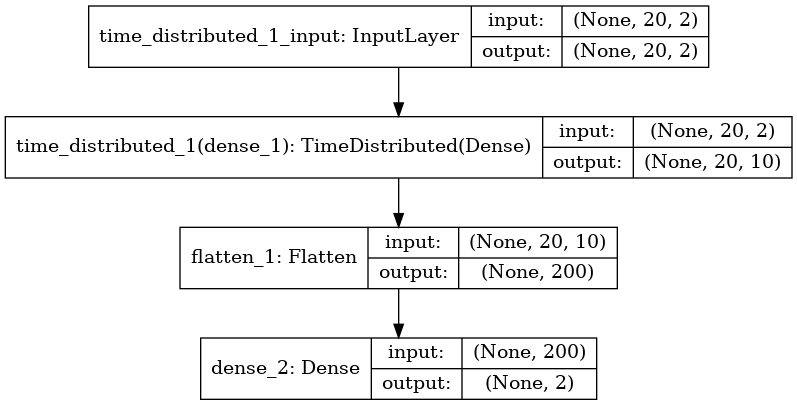
\includegraphics[width=0.8\textwidth]{ figures/net/NOREC_simple_mod.png}
			\caption{Estructura de \acrshort{mlp} con 1 capa oculta y 10 neuronas para imágenes modeladas.}
			\label{fig.norec_simple_mod}
		\end{center}
\end{figure}
\vspace{-10pt}

Tras la definición de la red, se realizan diversos experimentos con el objetivo de lograr la predicción en el escenario más complejo considerado. Se aumenta de forma progresiva la complejidad en el movimiento, considerando en primera instancia más grados de libertad, y posteriormente otras dinámicas.

\subsection{Influencia del número muestras}\label{ap.muestras}
Antes de comenzar con el estudio de las distintas redes con las dinámicas consideradas se realiza un breve estudio sobre el número de muestras utilizando el caso especial de la dinámica lineal, con pendiente nula, por su sencillez. Bajo esta premisa, se emplea en primer lugar un conjunto de 1000 muestras, de las cuales 800 se emplean para entrenamiento, 100 para validación y las 100 restantes para \textit{test}.\\

En la Figura~\ref{fig.norec_urm_fix_1000} se muestran los resultados obtenidos al evaluar la red entrenada con el conjunto cuya altura inicial del píxel en la imagen permanece fija.

\begin{figure}[H]
		\begin{center}
			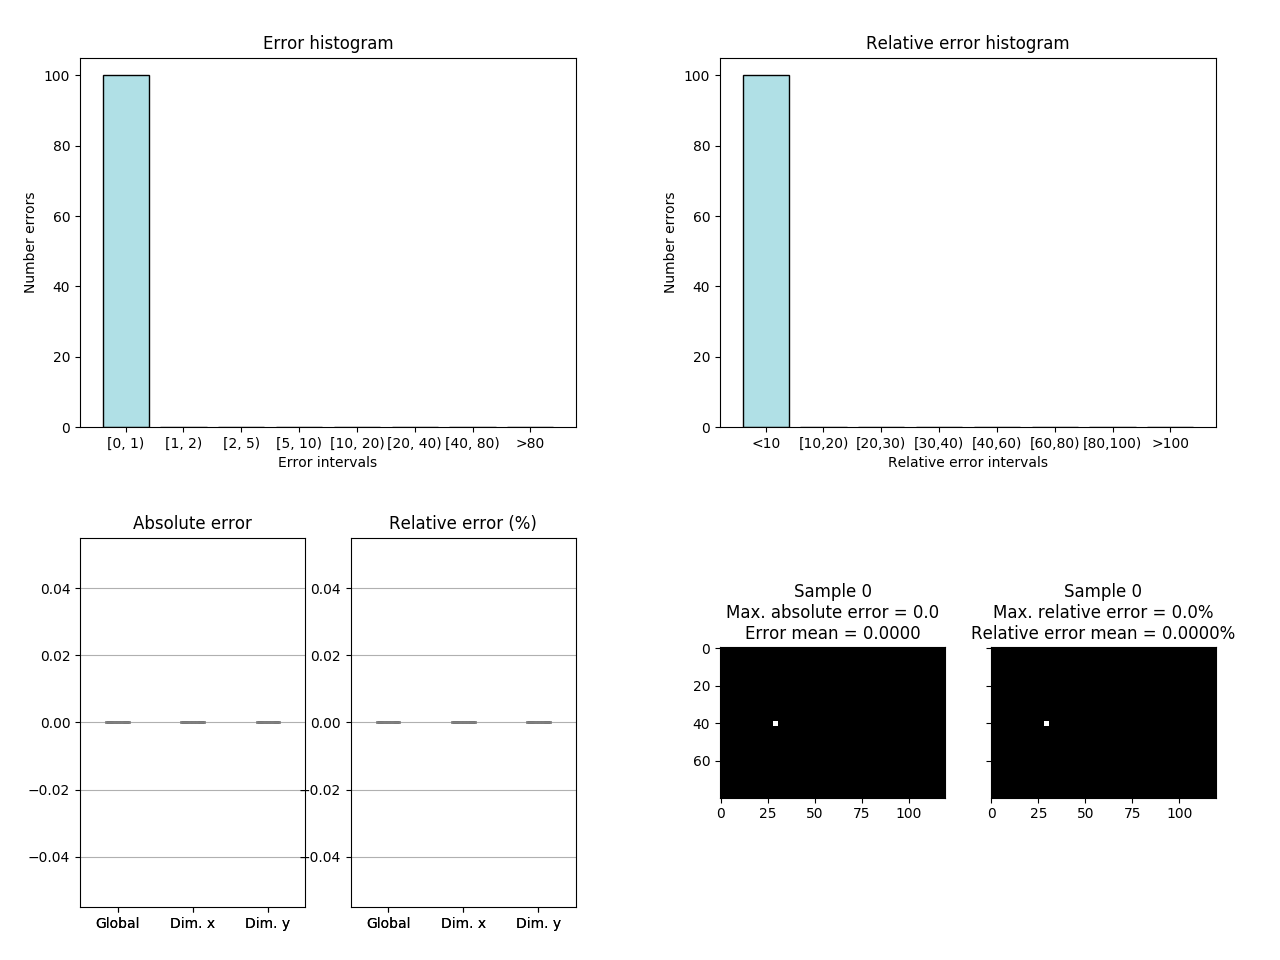
\includegraphics[width=0.8\textwidth]{ figures/test_mod/NOREC/URM_fix_1000.png}
			\caption{Resultados de \acrshort{mlp} con dinámica lineal, pendiente nula y altura fija en imágenes modeladas~(100 muestras de \textit{test})}
			\label{fig.norec_urm_fix_1000}
		\end{center}
\end{figure}
\vspace{-10pt}

El error obtenido en este caso es nulo ya que, al mantener fija la altura y aplicar las restricciones de aparición del píxel en todas la imágenes, el número de muestras distintas es mucho menor a las 1000 creadas. Este hecho hace que la red aprenda todos los ejemplos posibles en el entrenamiento, evitando que se pueda equivocar en cualquiera de los ejemplos de \textit{test}.\\

Con el objetivo de incrementar la complejidad de la dinámica, se entrena la misma estructura de red con el mismo número de muestras pero dejando la altura inicial como parámetro libre en cada predicción. Los resultados de la evaluación de esta nueva red, que se muestran en la Figura~\ref{fig.norec_urm_var_1000}, ya no son tan buenos como en el caso anterior. La razón es que, al dejar que la altura inicial tome un valor aleatorio ha aumentado la variabilidad de las muestras, impidiendo que la red vea la totalidad de las variantes en la fase de entrenamiento, presentando casos desconocidos en la evaluación.

\begin{figure}[H]
		\begin{center}
			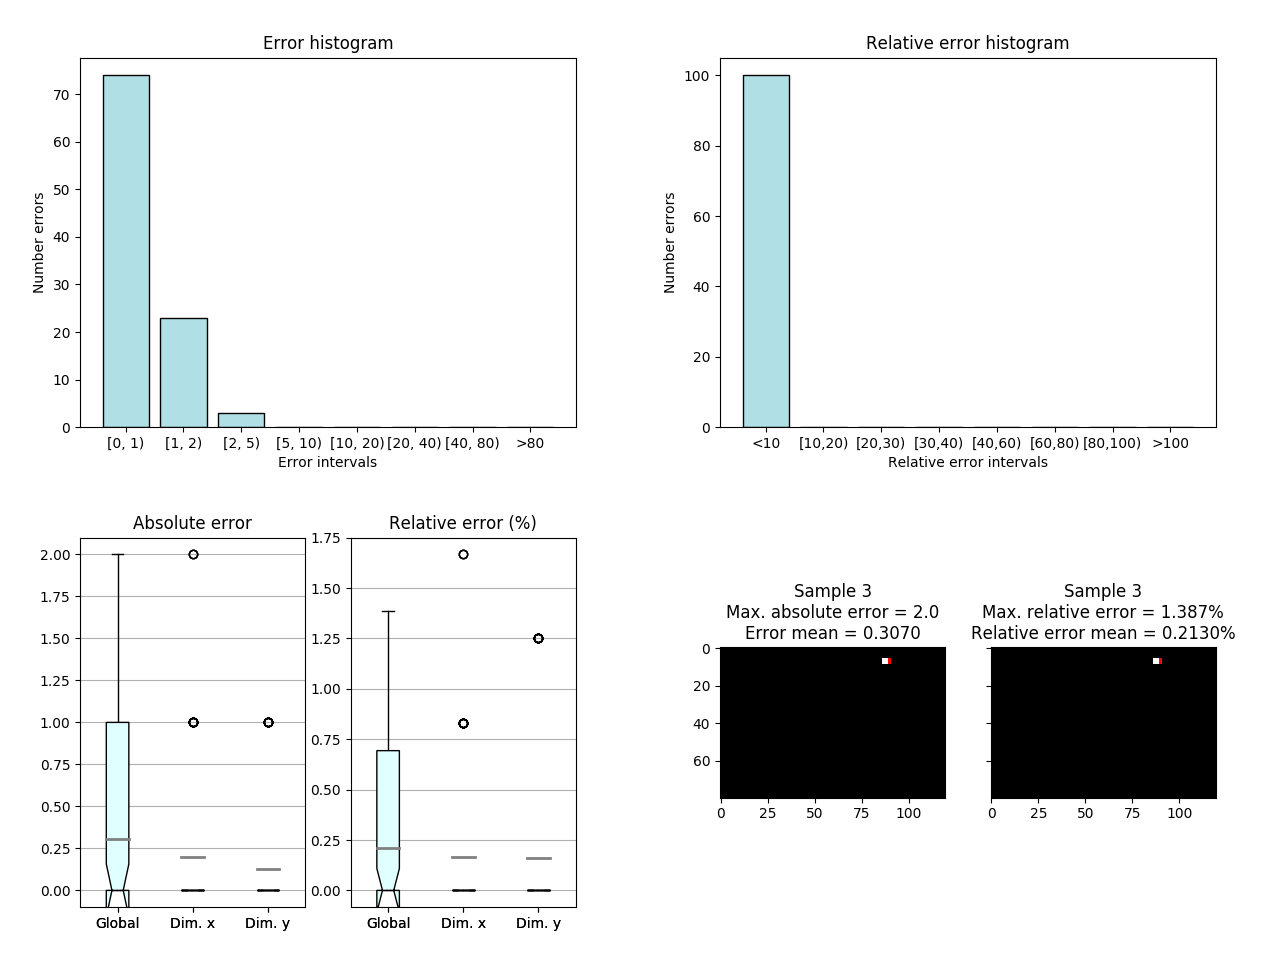
\includegraphics[width=0.8\textwidth]{ figures/test_mod/NOREC/URM_var_1000.png}
			\caption{Resultados de \acrshort{mlp} con dinámica lineal, pendiente nula y altura aleatoria en imágenes modeladas~(100 muestras de \textit{test}).}
			\label{fig.norec_urm_var_1000}
		\end{center}
\end{figure}
\vspace{-10pt}

La primera acción  para tratar de mejorar los resultados es aumentar el número de muestras para incrementar el número de ejemplos de los que la red aprende. En esta línea, se genera un nuevo conjunto de 5000 muestras con la misma proporción en la generación de las tres particiones: 4000 destinadas al entrenamiento, 500 a la validación y otras 500 al \textit{test}. Los resultados de la red entrenada con este nuevo conjunto se muestran en la Figura~\ref{fig.norec_urm_var_5000}, en la que se puede comprobar que el error vuelve a ser nulo.

\begin{figure}[H]
		\begin{center}
			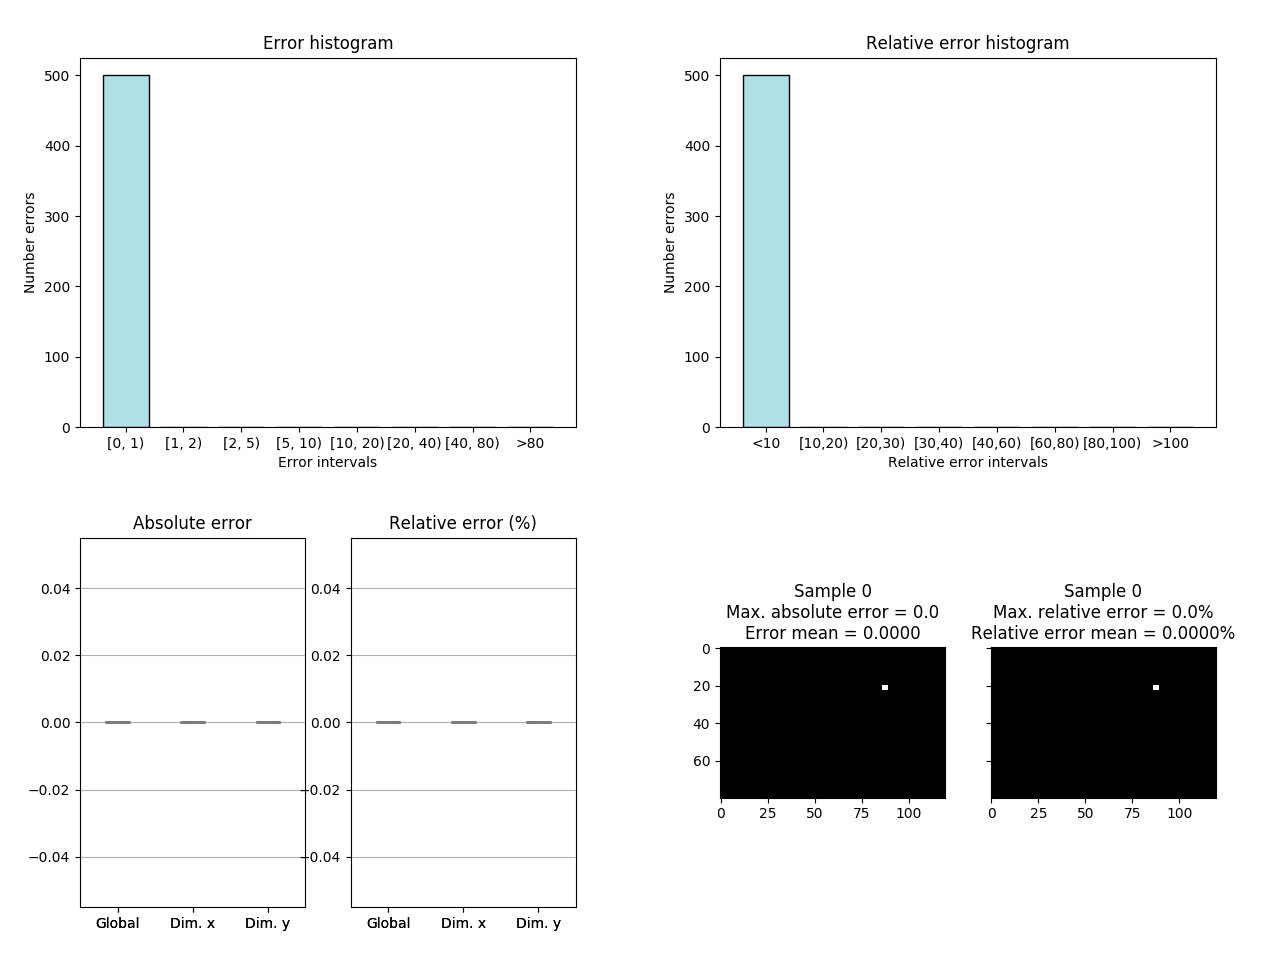
\includegraphics[width=0.8\textwidth]{ figures/test_mod/NOREC/URM_var_5000.png}
			\caption{Resultados de \acrshort{mlp} con dinámica lineal, pendiente nula y altura fija en imágenes modeladas~(500 muestras de \textit{test}).}
			\label{fig.norec_urm_var_5000}
		\end{center}
\end{figure}
\vspace{-10pt}

Con los resultados obtenidos se concluye que utilizar un mayor número de muestras es un factor que hace mejorar los resultados, pues la red aprende de una mayor variedad de ejemplos. Sin embargo, cuando se obtiene un acierto del 100\%, como en el primer caso, no hay margen de mejora y únicamente se consigue aumentar la complejidad computacional. Es decir, el aumento de muestras es un factor de mejora siempre que la naturaleza de las mismas sea lo suficientemente compleja como para necesitar un mayor número de observaciones para modelar la estadística subyacente en los datos.

\subsection{Predicción con dinámicas lineales}
Para abordar la predicción de fotogramas que representan objetos siguen una dinámica lineal se emplea un conjunto con un total de 10000 muestras dividido en 8000 muestras para entrenamiento, 1000 para validación y 1000 para evaluación.\\

En primer lugar se realiza el estudio de esta dinámica con un único \acrshort{dof}, la pendiente de la trayectoria del píxel activo, cuyos resultados de evaluación de la red entrenada queda reflejado en la Figura~\ref{fig.norec_lin_fix_10000}.

\begin{figure}[H]
		\begin{center}
			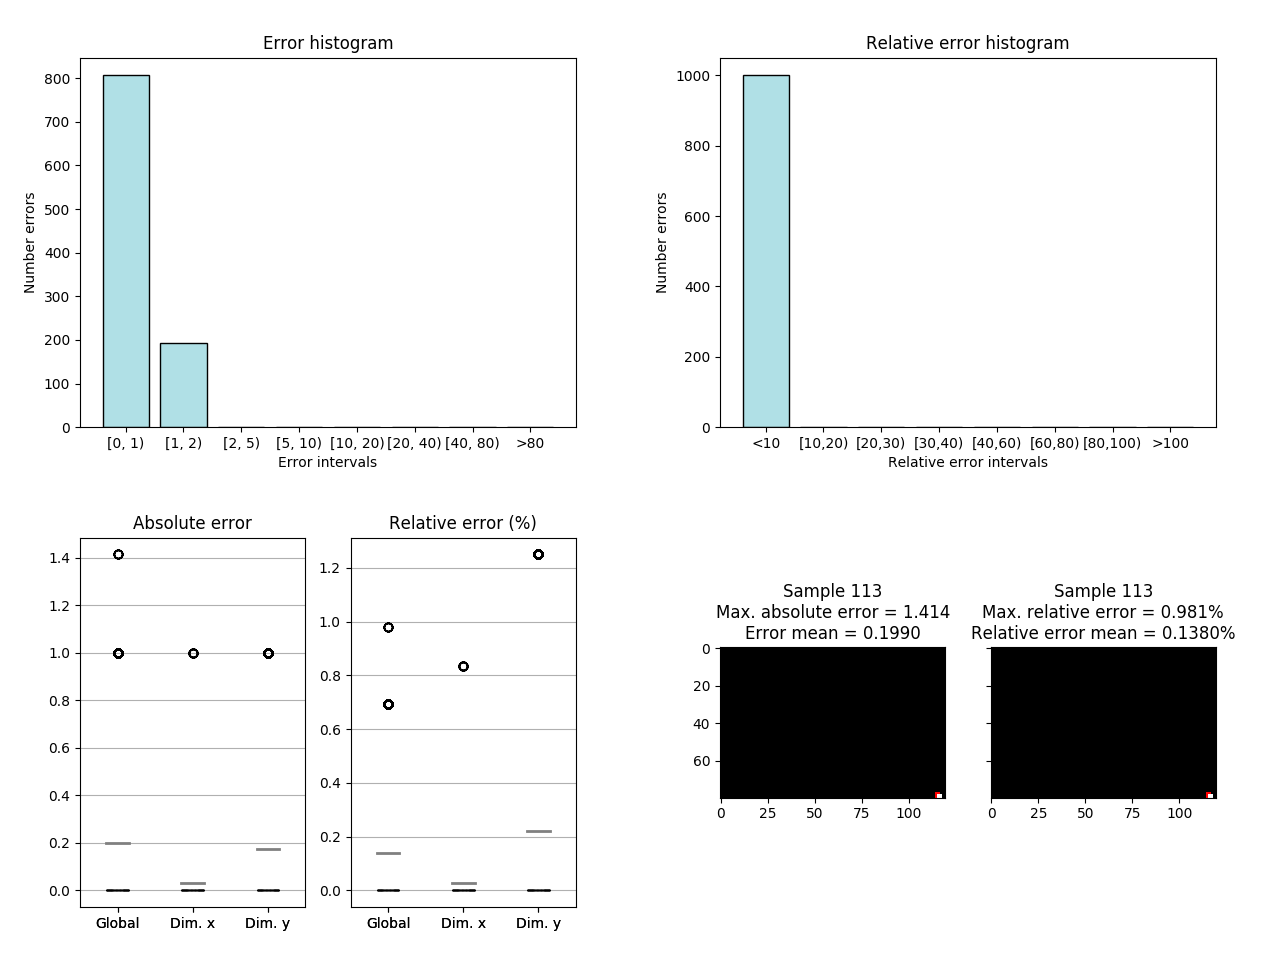
\includegraphics[width=0.8\textwidth]{ figures/test_mod/NOREC/linear_fix_10000.png}
			\caption{Resultados de \acrshort{mlp} con dinámica lineal de 1 \acrshort{dof} en imágenes modeladas~(1000 muestras de \textit{test}).} 
			\label{fig.norec_lin_fix_10000}
		\end{center}
\end{figure}
\vspace{-10pt}

Se puede comprobar que la capacidad de predicción de esta red es buena, ofreciendo un error relativo muy reducido tanto en términos de media como de máximo.\\

Se aumenta el grado de complejidad de la dinámica con un nuevo \acrshort{dof}, la altura inicial, y se repite el experimento con la misma estructura de red, cuyos resultados se reflejan en la Figura~\ref{fig.norec_lin_var_10000}. Como era de esperar, dejar mayor libertad de movimiento al píxel activo, aumentando la complejidad, repercute de forma directa en la capacidad de predicción de la red. Sin embargo, los resultados obtenidos indican que la red continúa siendo capaz de predecir bien bajo estas condiciones.\\

Dados los resultados para el caso más complejo de la dinámica lineal, 2~\acrshort{dof}, se concluye que, con el número de muestras modeladas establecidas y la estructura de red propuesta, es posible predecir satisfactoriamente la posición de un píxel móvil que sigue una dinámica lineal, independientemente de sus \acrshort{dof}.

\begin{figure}[H]
		\begin{center}
			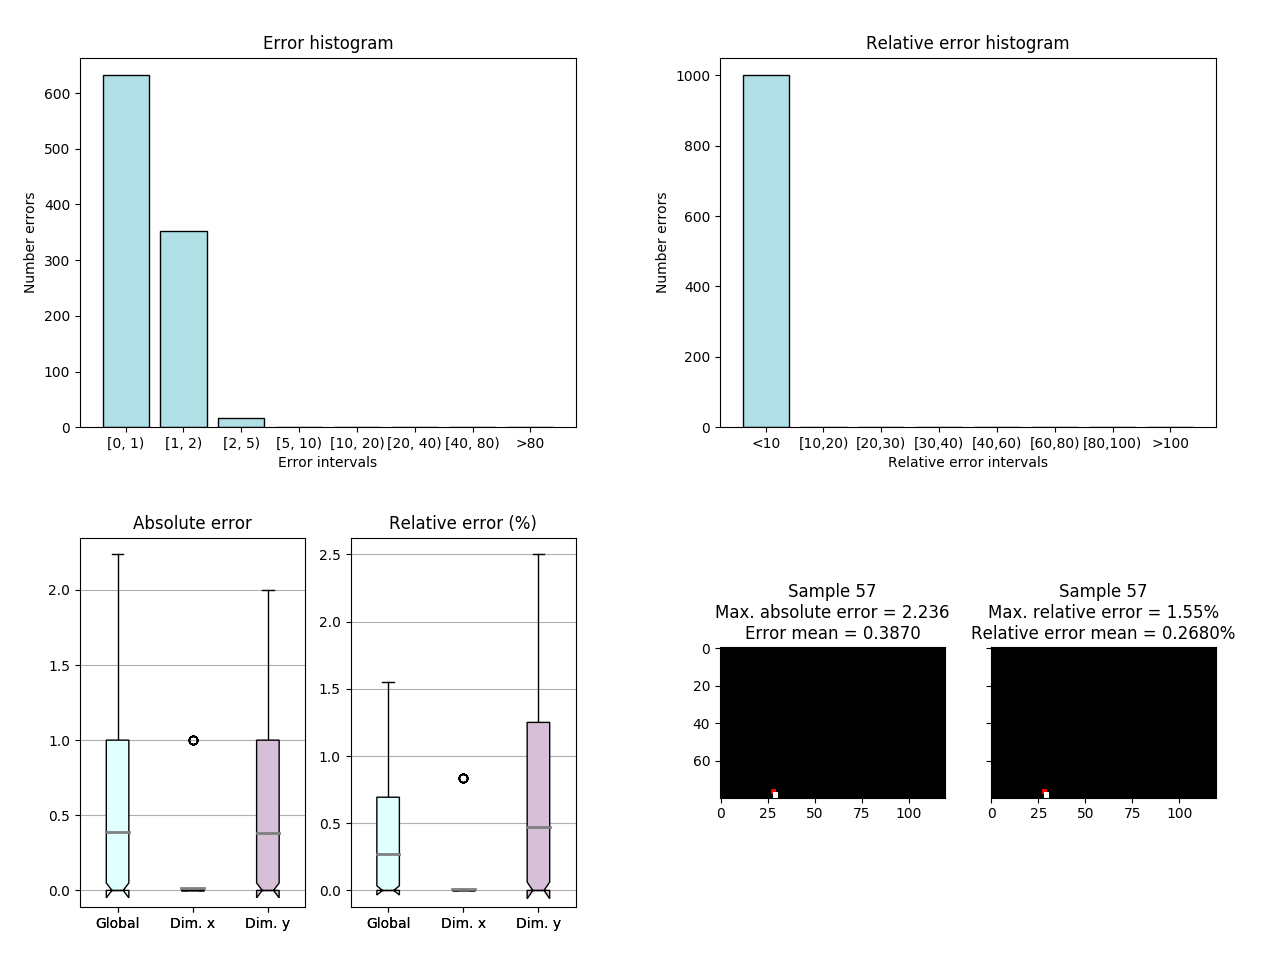
\includegraphics[width=0.8\textwidth]{ figures/test_mod/NOREC/linear_var_10000.png}
			\caption{Resultados de \acrshort{mlp} con dinámica lineal de 2 \acrshort{dof} en imágenes modeladas~(1000 muestras de \textit{test}).}
			\label{fig.norec_lin_var_10000}
		\end{center}
\end{figure}
\vspace{-10pt}


\subsection{Predicción con dinámicas parabólicas}
Para abordar la predicción de fotogramas que representan objetos siguen una dinámica parabólica se utiliza un conjunto con 10000 ejemplos, divididos de la misma manera que en la dinámica anterior.\\

El análisis de la capacidad predictiva de la red comienza con el caso más sencillo,  un único \acrshort{dof}, el valor de \textit{a} en esta dinámica. La Figura~\ref{fig.norec_parab_fix_10000} muestra los resultados obtenidos al evaluar la red entrenada bajo estas condiciones. Estos resultados demuestran que la red propuesta es capaz de predecir bien la posición del píxel móvil en este primer caso.

\begin{figure}[H]
		\begin{center}
			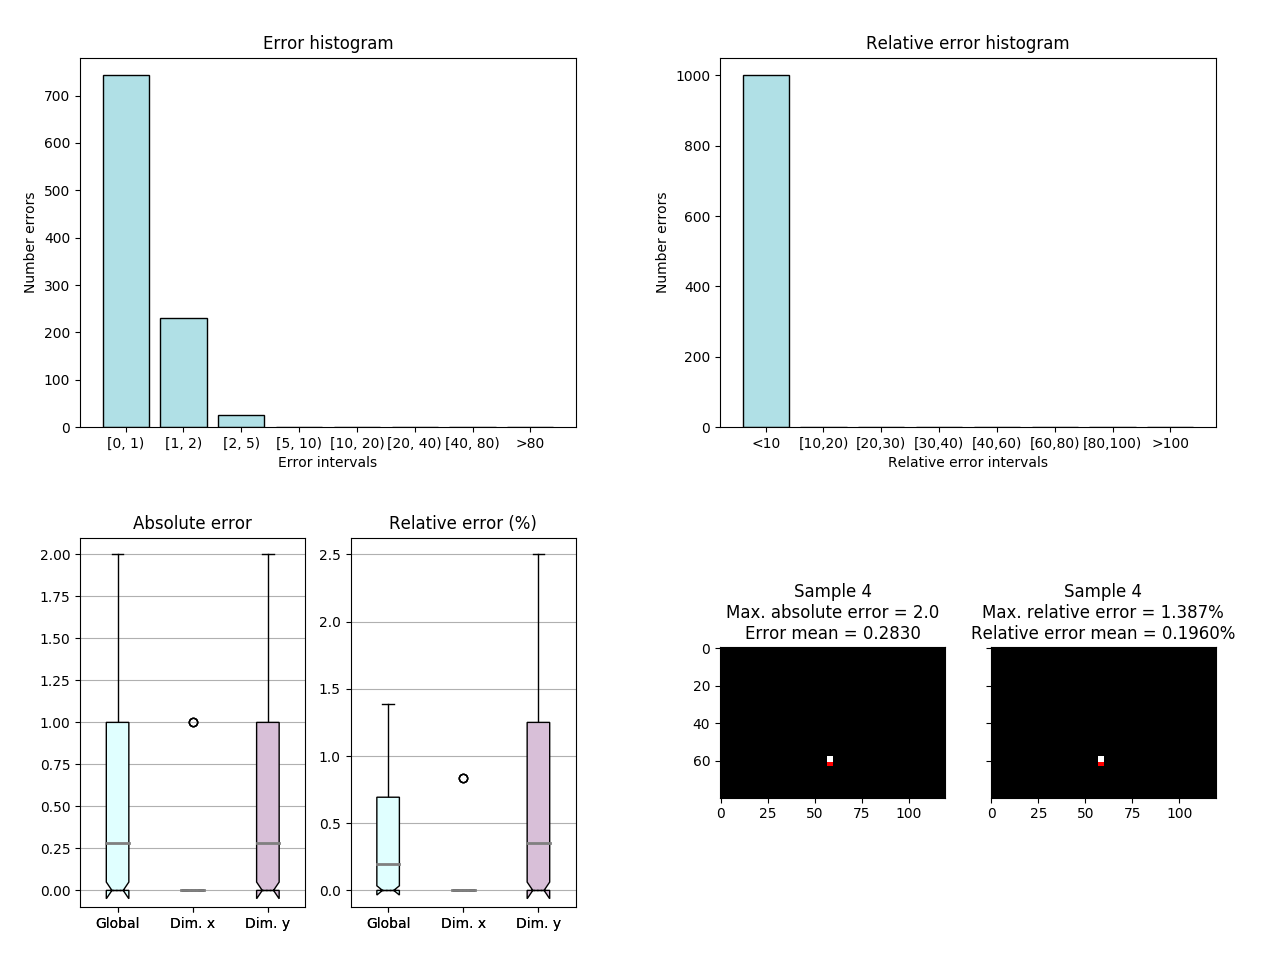
\includegraphics[width=0.8\textwidth]{ figures/test_mod/NOREC/parab_fix_10000.png}
			\caption{Resultados de \acrshort{mlp} con dinámica parabólica de 1 \acrshort{dof} en imágenes modeladas~(1000 muestras de \textit{test}).} 
			\label{fig.norec_parab_fix_10000}
		\end{center}
\end{figure}
\vspace{-10pt}

Tras los buenos resultados obtenidos con el primer caso de la dinámica, 1~\acrshort{dof},se prosigue con el aumento del los \acrshort{dof} para poner a prueba la estructura.\\

En las Figuras~\ref{fig.norec_parab_var_10000}~y~\ref{fig.norec_parab_var1_10000} se muestran los resultados obtenidos para las predicción de la dinámica con 2 y 3 \acrshort{dof}, la altura inicial y \textit{c}, respectivamente. A la vista de estos resultados se comprueba que, a pesar de que los resultados empeoran ligeramente al introducir más grados de libertad, éste se mantiene en unos valores razonables. Se concluye que, para imágenes modeladas, el \acrshort{mlp} es capaz de predecir el desplazamiento del píxel según la dinámica parabólica, independientemente del nivel de complejidad que se establezca.

\begin{figure}[H]
		\begin{center}
			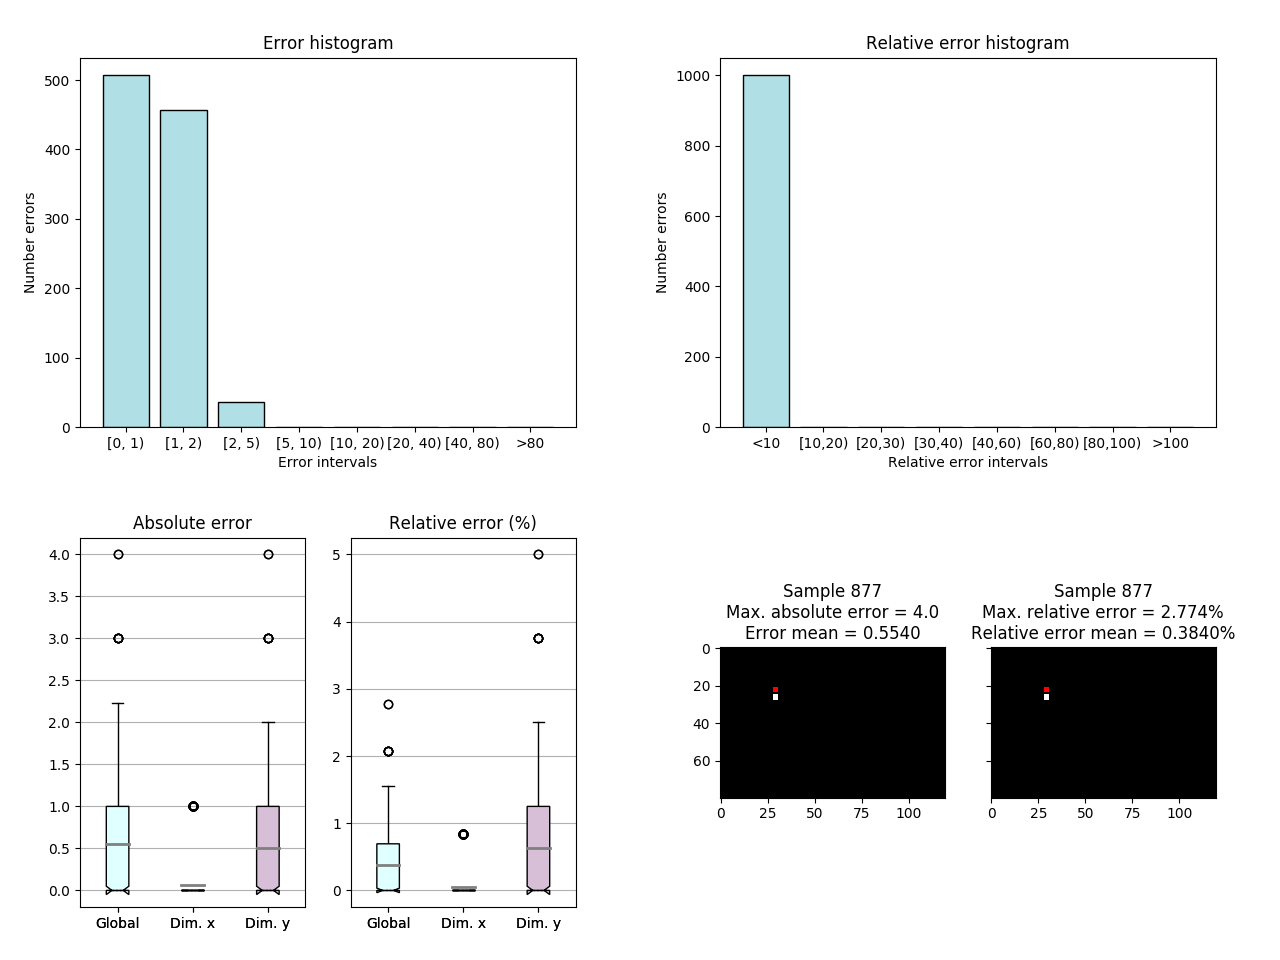
\includegraphics[width=0.8\textwidth]{ figures/test_mod/NOREC/parab_var_10000.png}
			\caption{Resultados de \acrshort{mlp} con dinámica parabólica de 2 \acrshort{dof} en imágenes ~(1000 muestras de \textit{test}).}
			\label{fig.norec_parab_var_10000}
		\end{center}
\end{figure}
\vspace{-30pt}
\begin{figure}[H]
		\begin{center}
			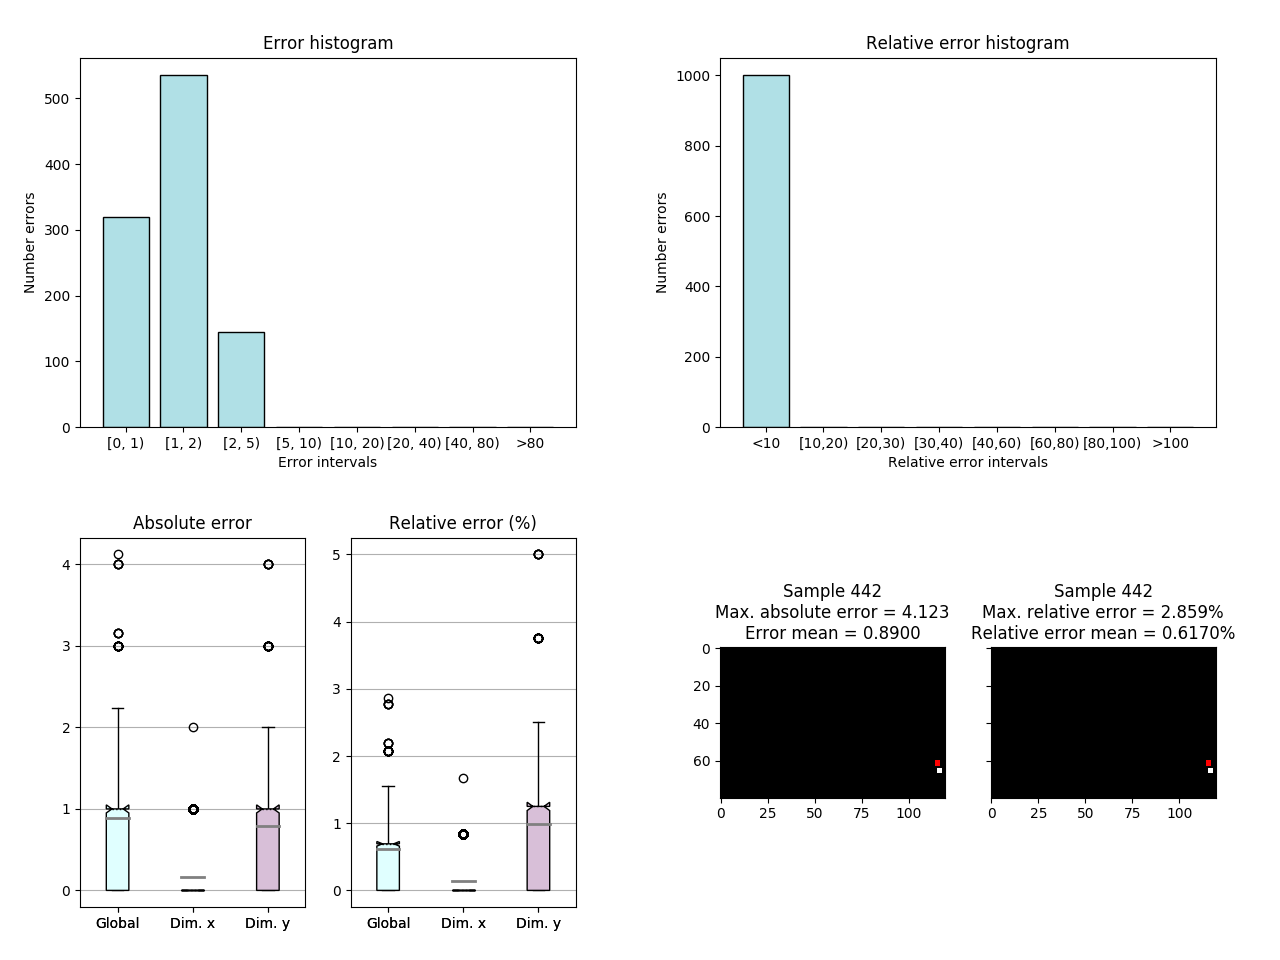
\includegraphics[width=0.8\textwidth]{ figures/test_mod/NOREC/parab_var1_10000.png}
			\caption{Resultados de \acrshort{mlp} con dinámica parabólica de 3 \acrshort{dof}~(1000 muestras de \textit{test}).}
			\label{fig.norec_parab_var1_10000}
		\end{center}
\end{figure}

\subsection{Predicción con dinámicas sinusoidales}
Para abordar la predicción de fotogramas que representan objetos siguen una dinámica sinusoidal se utiliza un \textit{dataset} compuesto por 10000 muestras, dividido de la misma forma que en dinámicas anteriores. En la Figura~\ref{fig.norec_sin_fix_10000} se muestra la evaluación de la estructura de red propuesta cuando el movimiento del píxel sigue una función sinusoidal con un solo \acrshort{dof}, la frecuencia.

\begin{figure}[H]
		\begin{center}
			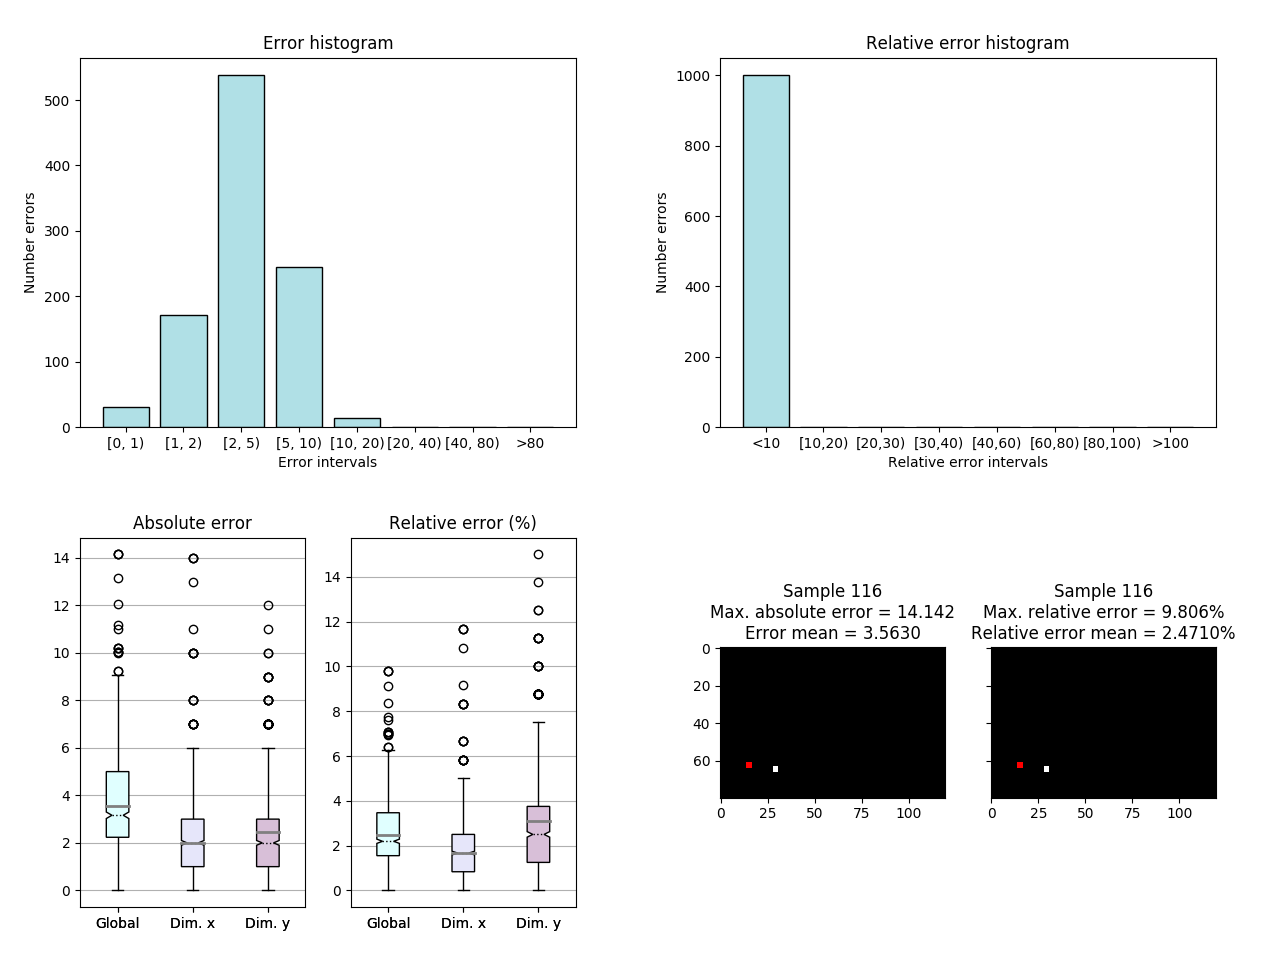
\includegraphics[width=0.8\textwidth]{ figures/test_mod/NOREC/sin_fix_10000.png}
			\caption{Resultados de \acrshort{mlp} con dinámica sinusoidal de 1 \acrshort{dof}~(1000 muestras de \textit{test})).} 
			\label{fig.norec_sin_fix_10000}
		\end{center}
\end{figure}
\vspace{-10pt}

En este caso, los resultados no son tan buenos como los obtenidos para las dinámicas anteriores, que eran más sencillas. Siguiendo la conclusión extraída del Apartado~\ref{ap.muestras}, la solución más inmediata a este deterioro es el aumento de muestras, pasando a un conjunto con un total del 100000 ejemplos: 80000 de entrenamiento, 10000 de validación y 10000 de \textit{test}. Los resultados obtenidos con este nuevo conjunto queda reflejado en los gráficos de la Figura~\ref{fig.norec_sin_fix_100000}.

\begin{figure}[H]
		\begin{center}
			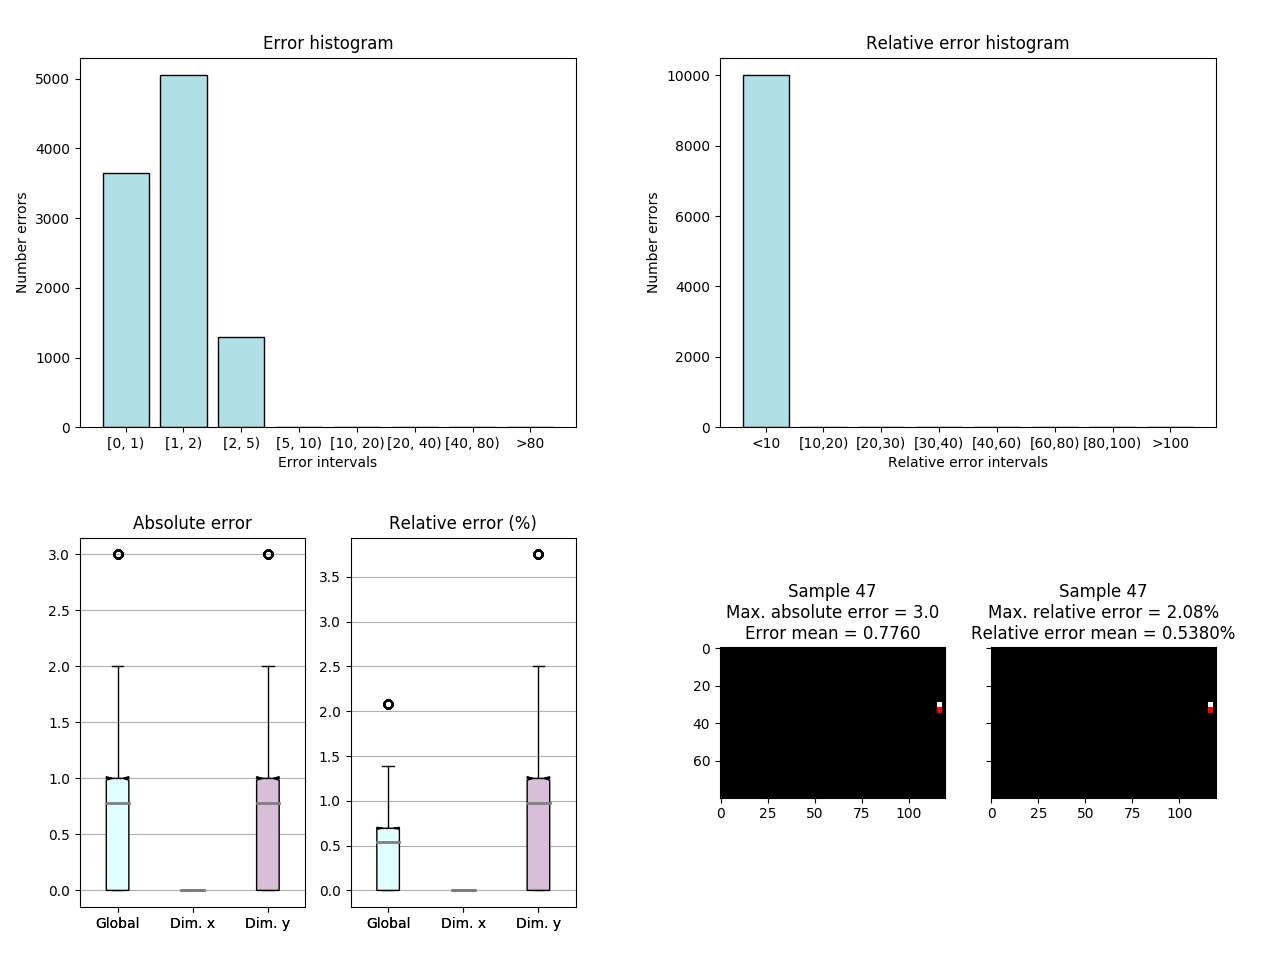
\includegraphics[width=0.8\textwidth]{ figures/test_mod/NOREC/sin_fix_100000.png}
			\caption{Resultados de \acrshort{mlp} con dinámica sinusoidal de 1 \acrshort{dof}~(10000 muestras de \textit{test}).}
			\label{fig.norec_sin_fix_100000}
		\end{center}
\end{figure}
\vspace{-10pt}

Con el incremento en el número de muestras se obtienen mejores resultados en la evaluación, alcanzando la capacidad predictiva conseguida en las dinámicas anteriores.\\

Manteniendo en 100000 el número de muestras, se aumenta la libertad de movimiento del píxel a 2 \acrshort{dof}, con la altura inicial. La red se entrena y evalúa bajo estas premisas dando lugar a los resultados mostrados en la Figura~\ref{fig.norec_sin_var_100000}. Estos datos hacen ver que el aumento de un grado de libertad en esta dinámica incrementa de forma significativa su complejidad, perdiendo la red la capacidad predictiva alcanzada.

\begin{figure}[H]
		\begin{center}
			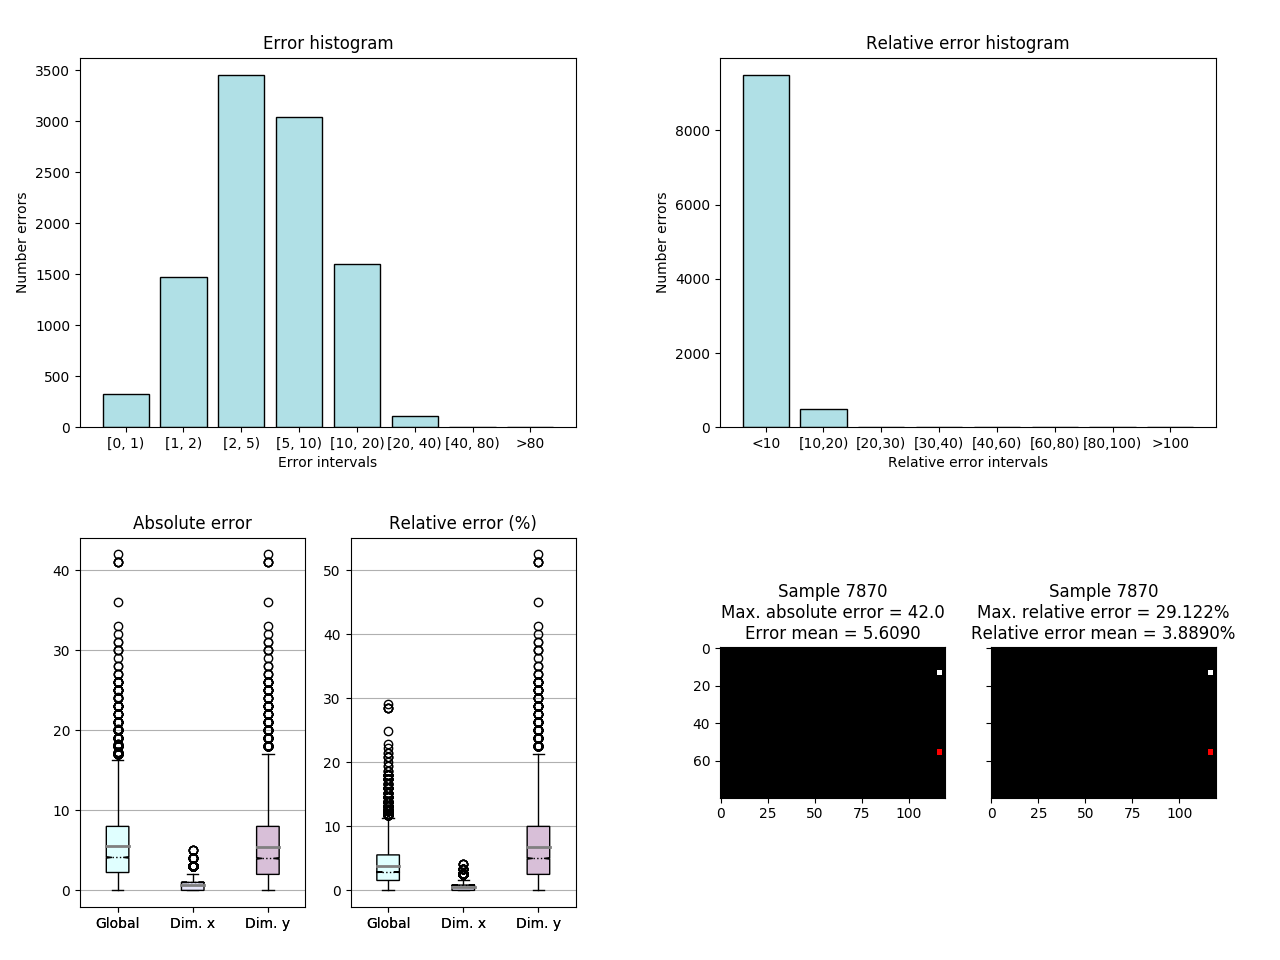
\includegraphics[width=0.8\textwidth]{ figures/test_mod/NOREC/sin_var_100000.png}
			\caption{Resultados de \acrshort{mlp} con dinámica sinusoidal de 2 \acrshort{dof}~(10000 muestras de \textit{test}).}
			\label{fig.norec_sin_var_100000}
		\end{center}
\end{figure}
\vspace{-10pt}

Con estos resultados se concluye que la estructura del \acrshort{mlp} propuesto no es capaz de abarcar la dinámica sinusoidal en su totalidad, poniendo su límite en un único \acrshort{dof}.

\subsection{Resumen de resultados} \label{ap.resumen_RNNmlp}
En la Tabla~\ref{tab.mlp} se muestra un resumen de los resultados alcanzados en cada dinámica.

\begin{table}[H]
	\centering
	\begin{tabular}{{|l|c|c|}}
		\hline
		\multicolumn{2}{|c|}{\textbf{Dinámica}} & \textbf{\acrshort{mlp}}\\ \hline 
		\multirow{2}{*}{Lineal}
		&1~\acrshort{dof} & \cellcolor{darkgreen}{0.21\%}\\
		\cline{2-3}
        &2~\acrshort{dof} & \cellcolor{darkgreen}{0.31\%}\\
        \hline
        \multirow{3}{*}{Parabólica}
        &1~\acrshort{dof} & \cellcolor{darkgreen}0.28\%\\
        \cline{2-3}
        &2~\acrshort{dof} & \cellcolor{darkgreen}0.42\%\\
        \cline{2-3}
        &3~\acrshort{dof} & \cellcolor{darkgreen}0.65\%\\ 
        \hline
        \multirow{2}{*}{Sinusoidal}
        &1~\acrshort{dof} & \cellcolor{darkgreen}0.54\%\\
        \cline{2-3}
        &2~\acrshort{dof} & \cellcolor{myorange}3.89\%\\
        \hline
	\end{tabular}
	\caption{Promedio del error relativo en \textit{test} al evaluar el \acrshort{mlp} con imágenes modeladas y distintas dinámicas (10000 muestras de \textit{test}).}
	\label{tab.mlp}
\end{table}

Para la interpretación de esta tabla se ha establecido un código de cuatro colores que indiquen a simple vista los mejores resultados, en términos de promedio y máximo de error relativo, para cada uno de los casos:

\begin{itemize}
    \item \textbf{Verde oscuro:} Indica muy buenos resultados.
    \item \textbf{Verde claro:} Indica resultados satisfactorios con cierto grado de mejoría.
    \item \textbf{Naranja:} Indica resultados intermedio, generalmente con un buen valor promedio pero un máximo elevado.
    \item \textbf{Rojo:} Indica malos resultados.
\end{itemize}

Además, en el interior de cada celda se refleja el promedio del error relativo de cada uno de los casos para una ilustración cuantitativa de los resultados. Con el objetivo de obtener una evaluación equitativa se han evaluado todas las redes con un conjunto de 10000 muestras, repitiendo la evaluación en aquellas que se utilizaron 1000.
\section{Arquitectura recurrente: LSTM-1}
Otro punto de estudio en el trabajo es el análisis de la capacidad de predicción con redes recurrentes, capaces de captar la relación temporal. Más concretamente se ha optado por el uso de las \acrshort{lstm}, explicadas en el Apartado~\ref{ap.lstm}, por su uso extendido en problemas de esta tipología. En la Figura~\ref{fig.rec_simple_mod} se muestra la estructura de red creada para el caso más sencillo, en el que se emplea una única capa \acrshort{lstm} de 25 neuronas.
\vspace{10pt}
\begin{figure}[H]
		\begin{center}
			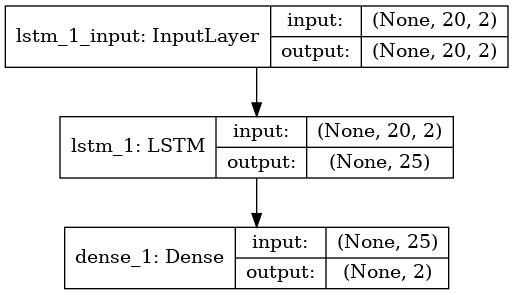
\includegraphics[width=0.6\textwidth]{ figures/net/REC_simple_mod.png}
			\caption{Estructura de LSTM-1 para imágenes modeladas.}
			\label{fig.rec_simple_mod}
		\end{center}
\end{figure}
\vspace{-10pt}

Las entradas y la salida de esta nueva estructura de red coinciden con las establecidas para el \acrshort{mlp}: 20 posiciones como entrada y 1 como salida.

\subsection{Predicción con dinámicas lineales}
Al aplicar la red recurrente sobre los \textit{dataset} cuyo movimiento del píxel en la imagen se rige por la función lineal se obtienen unos resultados muy similares que en el caso no recurrente. En las Figuras~\ref{fig.rec_lin_fix_10000}~y~\ref{fig.rec_lin_var_10000} se puede comprobar cómo se obtienen resultados muy similares a los del \acrshort{mlp}, mejorando ligeramente los resultados en términos de media.\\

\begin{figure}[H]
		\begin{center}
			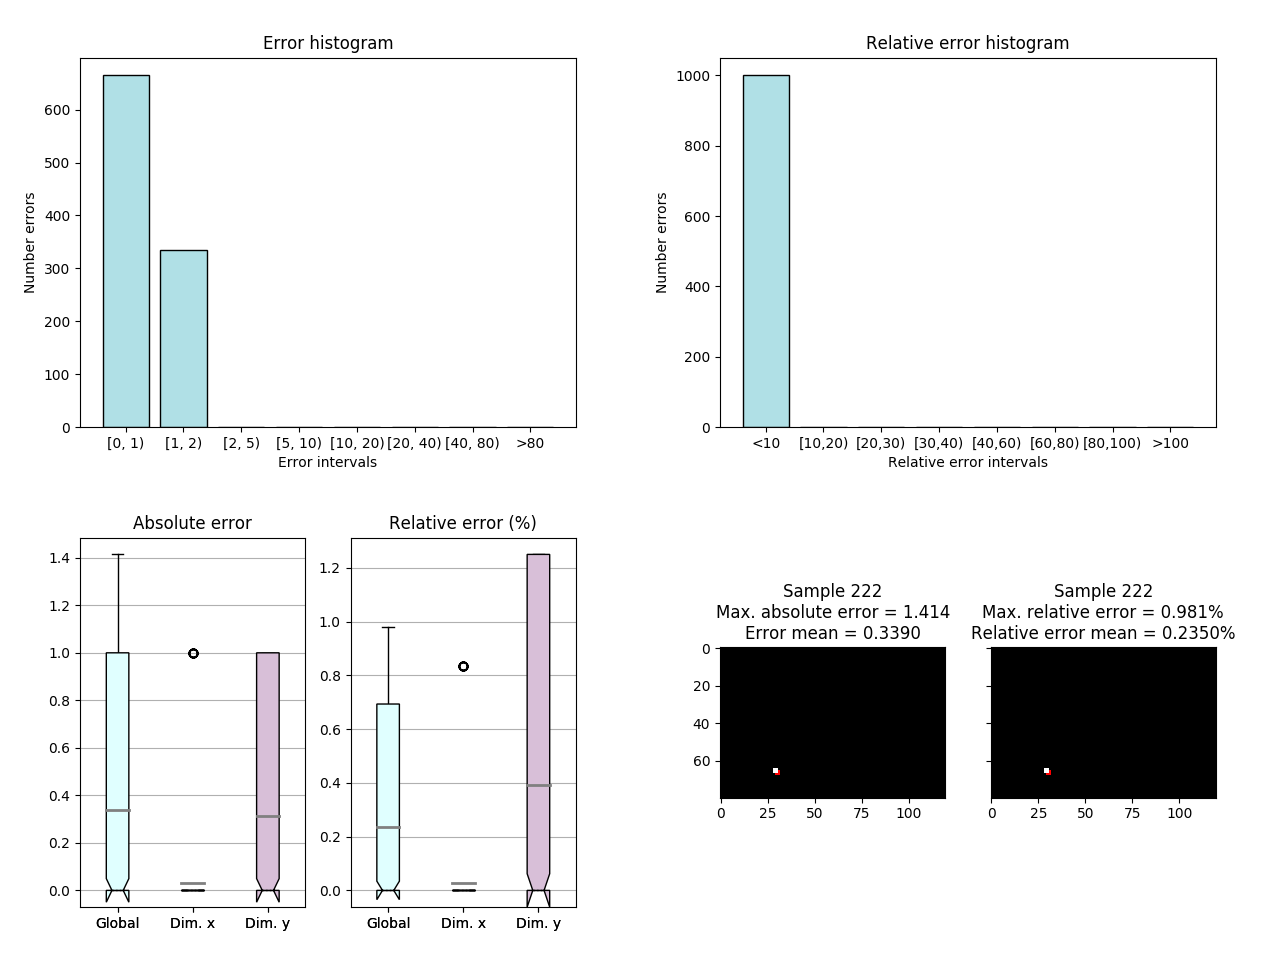
\includegraphics[width=0.8\textwidth]{ figures/test_mod/REC/simple/linear_fix_10000.png}
			\caption{Resultados de LSTM-1 con dinámica lineal de 1 \acrshort{dof}~(1000 muestras de \textit{test}).} 
			\label{fig.rec_lin_fix_10000}
		\end{center}
\end{figure}

\begin{figure}[H]
		\begin{center}
			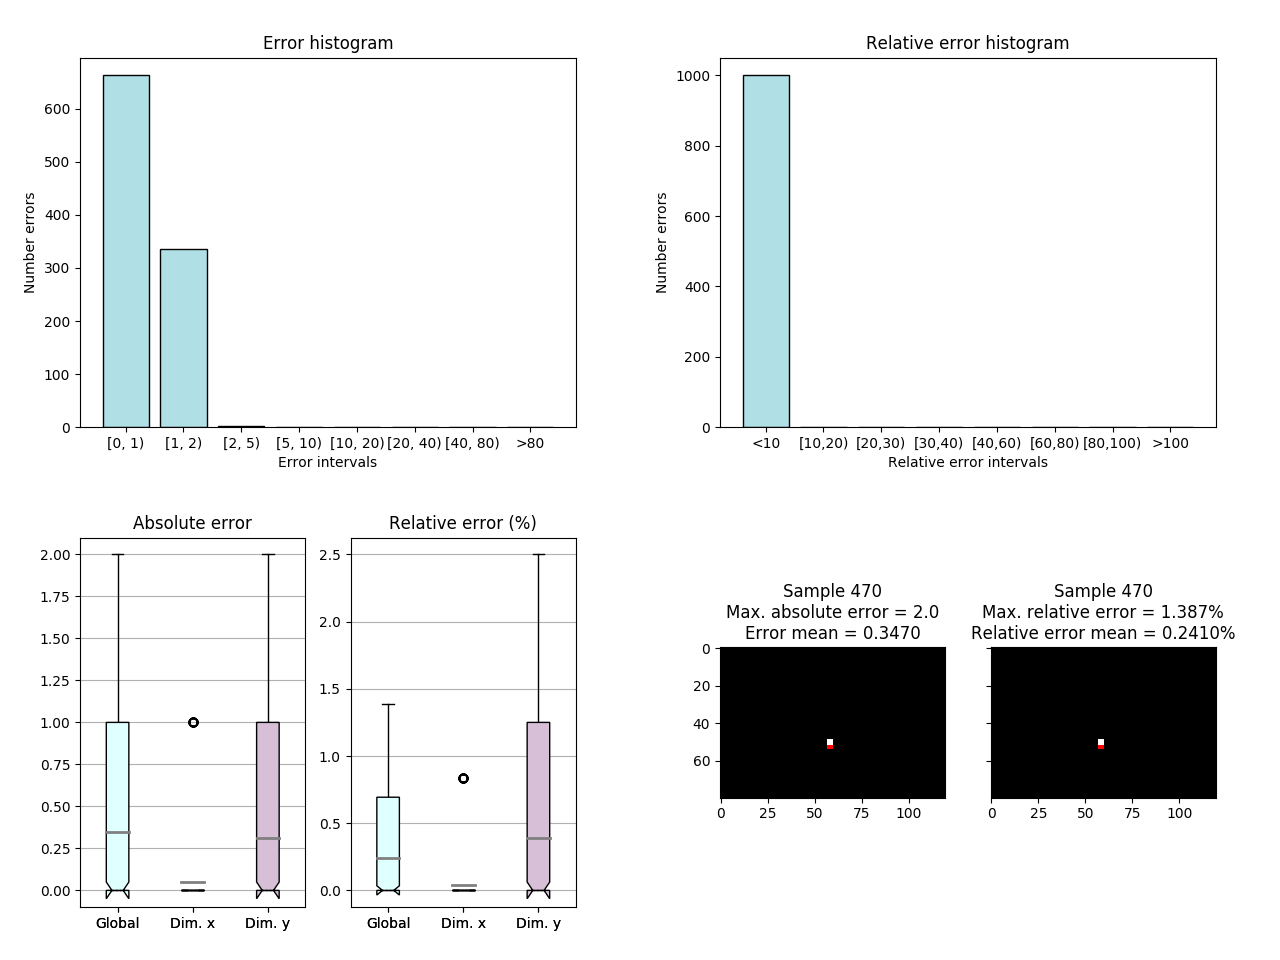
\includegraphics[width=0.8\textwidth]{ figures/test_mod/REC/simple/linear_var_10000.png}
			\caption{Resultados de LSTM-1 con dinámica lineal de 2 \acrshort{dof}~(1000 muestras de \textit{test}).}
			\label{fig.rec_lin_var_10000}
		\end{center}
\end{figure}
\vspace{-10pt}

Estos resultados permiten concluir que en las dinámicas cuyos resultados en el \acrshort{mlp} son buenos, al utilizar redes \acrshort{lstm} la capacidad predictiva se mantiene. Es decir, las redes recurrentes no empeoran significativamente la predicción cuándo ésta funciona sin recurrencia.

\subsection{Predicción con dinámicas parabólicas}
El caso parabólico es muy similar al lineal. Con la red no recurrente ya se consigue que la capacidad predictiva sea buena, por lo que introducir la recurrencia no aportará gran diferencia aunque puede mejorar los resultados. En la Tabla~\ref{tab.mlp_lstm_parab} se muestra una comparación de los resultados obtenidos para esta dinámica con sus 3~\acrshort{dof} y 10000 muestras, tanto con la estructura \acrshort{mlp} como con la \acrshort{lstm}.\\

Estos resultados corroboran lo concluido en el caso lineal: introducir la recurrencia en los casos donde se obtenían buenos resultados, no modifica significativamente los mismos.

\begin{table}[H]
	\centering
	\begin{tabular}{{l|c|c|c|c|}}
		\cline{2-5}
		& \multicolumn{2}{|c|}{\textbf{\acrshort{mlp}}} & \multicolumn{2}{|c|}{\textbf{LSTM-1}} \\
		\hline
		\multicolumn{1}{|l|}{\textbf{\acrshort{dof}}} & \textbf{\textit{Max.}} & \textbf{\textit{Mean}} & \textbf{\textit{Max.}} & \textbf{\textit{Mean}}\\
		\hline 
		\multicolumn{1}{|l|}{\textbf{1~(\textit{a})}} & 1.4\% & 0.2\% & 1.4\% & 0.1\%\\ \hline
		\multicolumn{1}{|l|}{\textbf{2~(\textit{c})}} & 2.8\% & 0.4\% & 2.2\% & 0.3\%\\ \hline
		\multicolumn{1}{|l|}{\textbf{3~(\textit{b})}} & 2.9\% & 0.6\% & 2.3\% & 0.6\%\\ \hline
	\end{tabular}
	\caption{Error relativo en la dinámica parabólica con \acrshort{mlp} y LSTM-1 (1000 muestras de \textit{test})).}
	\label{tab.mlp_lstm_parab}
\end{table}

\subsection{Predicción con dinámicas sinusoidales}
En la dinámica sinusoidal, con el \acrshort{mlp}, únicamente se conseguía dominar el caso más sencillo de 1 \acrshort{dof} (frecuencia). En la Figura~\ref{fig.rec_sin_fix_100000} se muestran los resultados obtenidos para este caso utilizando la estructura recurrente propuesta. Se mantienen los buenos resultados arrojados por el \acrshort{mlp}, reforzando las conclusiones extraídas.\\

\begin{figure}[H]
		\begin{center}
			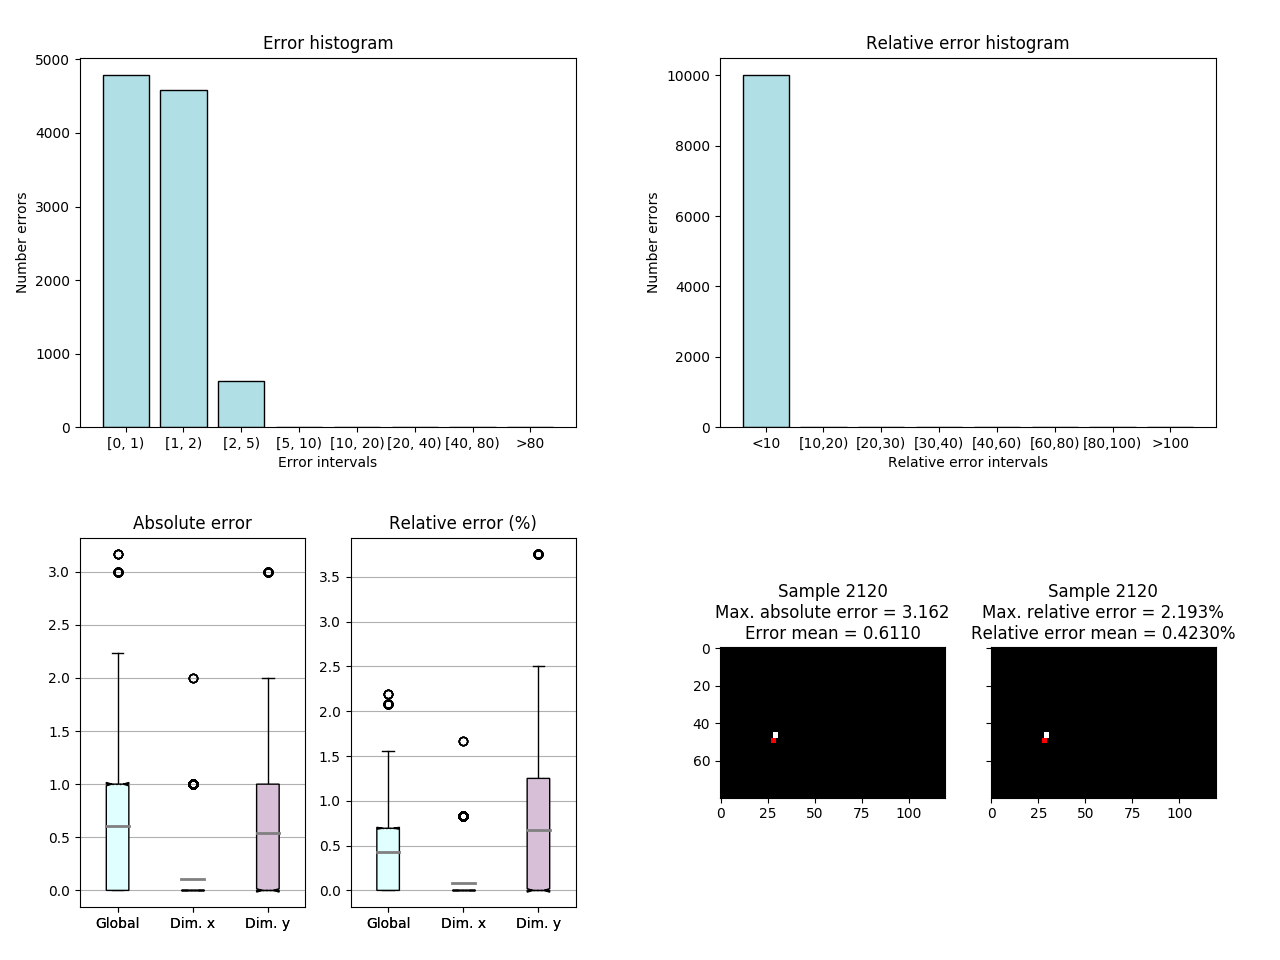
\includegraphics[width=0.8\textwidth]{ figures/test_mod/REC/simple/sin_fix_100000.png}
			\caption{Resultados de LSTM-1 con dinámica sinusoidal de 1 \acrshort{dof}~(10000 muestras de \textit{test}).}
			\label{fig.rec_sin_fix_100000}
		\end{center}
\end{figure}

Al complicar la dinámica con el aumento de la libertad de movimiento del píxel, la red no recurrente estudiada no es capaz de predecir correctamente. Se espera que al introducir la recurrencia, no solo se mantengan los resultados como anteriormente, sino que la capacidad predictiva en estos casos mejore considerablemente. En la Figura~\ref{fig.rec_sin_var_100000} se muestran los resultados del primer experimento en este sentido. Se entrena y evalúa la red recurrente propuesta con un conjunto de 100000 muestras y permitiendo 2 \acrshort{dof}, frecuencia y altura inicial.

\begin{figure}[H]
		\begin{center}
			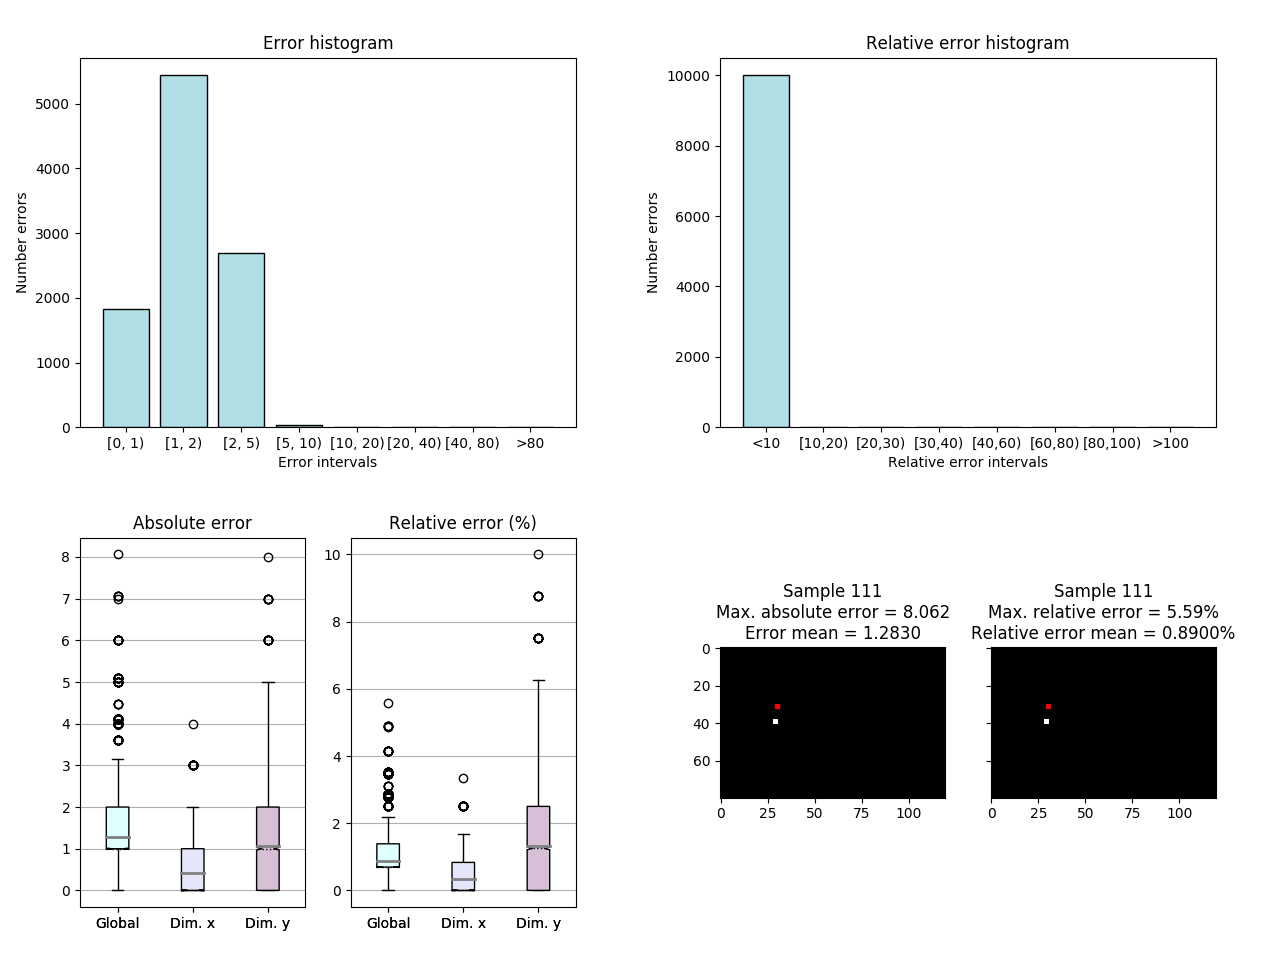
\includegraphics[width=0.8\textwidth]{ figures/test_mod/REC/simple/sin_var_100000.png}
			\caption{Resultados de LSTM-1 con dinámica sinusoidal de 2 \acrshort{dof}~(10000 muestras de \textit{test}).}
			\label{fig.rec_sin_var_100000}
		\end{center}
\end{figure}
\vspace{-10pt}

Se puede observar una mejora considerable respecto a los resultados de la Figura~\ref{fig.norec_sin_var_100000}, que evalúa una red no recurrente bajo las mismas circunstancias. Esta comparación corrobora la idea mencionada anteriormente de que la recurrencia mejora la capacidad predictiva de una red cuando esta no es es del todo buena.\\

Se añade un nuevo \acrshort{dof} a la dinámica, la amplitud y se realiza el entrenamiento y evaluación con un conjunto del mismo número de muestras~(100000) que en los casos anteriores. En la Figura~\ref{fig.rec_sin_var1_100000} se muestran los resultados para este caso.

\begin{figure}[H]
		\begin{center}
			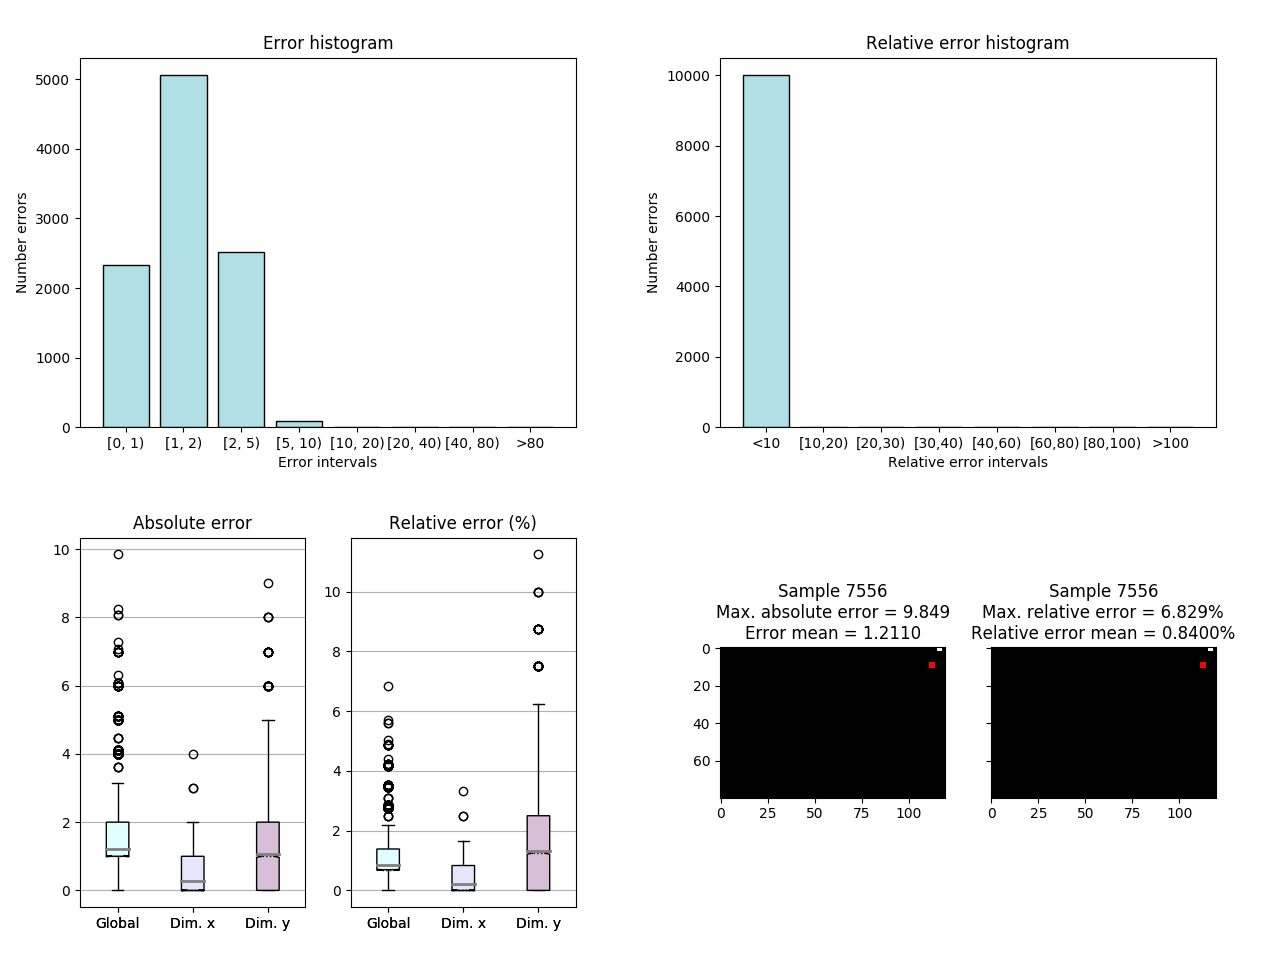
\includegraphics[width=0.8\textwidth]{ figures/test_mod/REC/simple/sin_var1_100000.png}
			\caption{Resultados de LSTM-1 con dinámica sinusoidal de 3 \acrshort{dof}~(10000 muestras de \textit{test}).}
			\label{fig.rec_sin_var1_100000}
		\end{center}
\end{figure}
\vspace{-10pt}

Los resultados obtenidos indican que la red tiene una buena capacidad predictiva, lo que refuerza la idea de que introducir la recurrencia en problemas de esta naturaleza facilita la tarea de predicción.\\

Se entrena la red con el siguiente grado de complejidad, 4~\acrshort{dof}, cuyos resultados se reflejan en la Figura~\ref{fig.rec_sin_var2_100000}. Para este último caso, el más complejo de la dinámica, la red no tiene una buena capacidad predictiva a pesar de introducir la recurrencia. Este hecho puede derivarse de la sencillez de la propia red propuesta, que dispone de una única capa con 25 neuronas, algo que se tratará posteriormente.

\begin{figure}[H]
		\begin{center}
			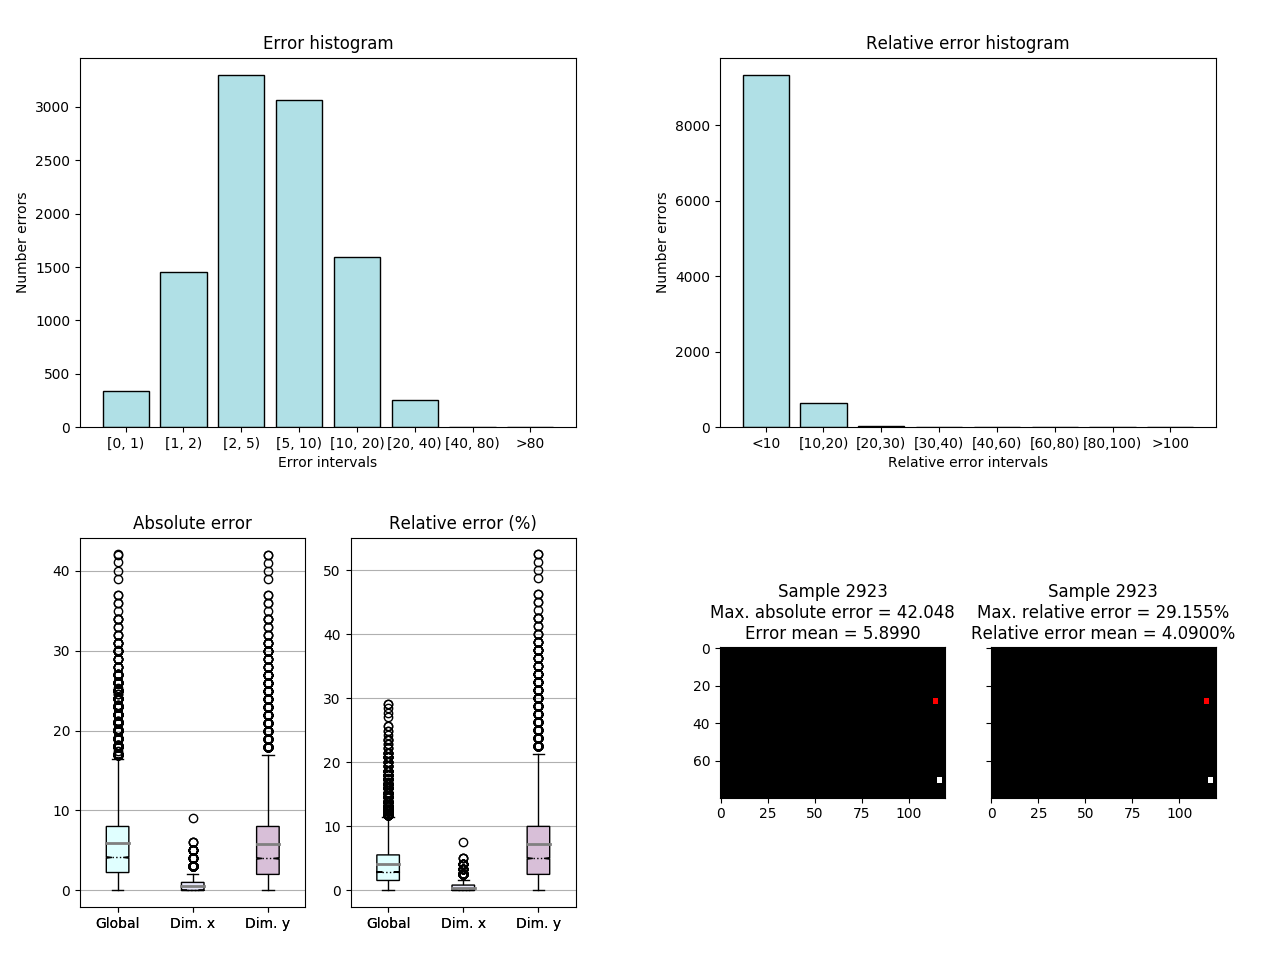
\includegraphics[width=0.8\textwidth]{ figures/test_mod/REC/simple/sin_var2_100000.png}
			\caption{Resultados de LSTM-1 con dinámica sinusoidal de 4 \acrshort{dof}~(10000 muestras de \textit{test}).}
			\label{fig.rec_sin_var2_100000}
		\end{center}
\end{figure}
\vspace{-20pt}
\subsection{Resumen de resultados}
La Tabla~\ref{tab.lstm1} resume los resultados obtenidos con la red \textit{LSTM-1} para cada dinámica.

\begin{table}[H]
	\centering
	\begin{tabular}{{|l|c|c|}}
		\hline
		\multicolumn{2}{|c|}{\textbf{Dinámica}} & \textbf{LSTM-1}\\ \hline 
		\multirow{2}{*}{Lineal}
		&1~\acrshort{dof} & \cellcolor{darkgreen}0.16\%\\
		\cline{2-3}
        &2~\acrshort{dof} & \cellcolor{darkgreen}0.25\%\\ 
        \hline
        \multirow{3}{*}{Parabólica}
        &1~\acrshort{dof} & \cellcolor{darkgreen}0.12\%\\
        \cline{2-3}
        &2~\acrshort{dof} & \cellcolor{darkgreen}0.35\%\\
        \cline{2-3}
        &3~\acrshort{dof} & \cellcolor{darkgreen}0.58\%\\ 
        \hline
        \multirow{4}{*}{Sinusoidal}
        &1~\acrshort{dof} & \cellcolor{darkgreen}0.42\%\\
        \cline{2-3}
        &2~\acrshort{dof} & \cellcolor{greenyellow}0.89\%\\
        \cline{2-3}
        &3~\acrshort{dof} & \cellcolor{greenyellow}0.84\%\\
        \cline{2-3}
        &4~\acrshort{dof} & \cellcolor{myorange}4.1\%\\ 
        \hline
	\end{tabular}
	\caption{Promedio del error relativo en \textit{test} al evaluar la red LSTM-1 con imágenes modeladas y distintas dinámicas (10000 muestras de \textit{test}).}
	\label{tab.lstm1}
\end{table}

Al igual que en el caso anterior se han evaluado todas las redes con un conjunto de 10000 muestras para una comparación equitativa, repitiendo la evaluación en aquellas que se utilizaron 1000.

\section{Arquitectura recurrente: LSTM-4}
Para tratar de obtener una arquitectura capaz de predecir en todas las dinámicas en su caso más complejo se realizan una serie de experimentos que dan lugar a la estructura recurrente definida en la Figura~\ref{fig.rec_complex_mod}.

\begin{figure}[H]
		\begin{center}
			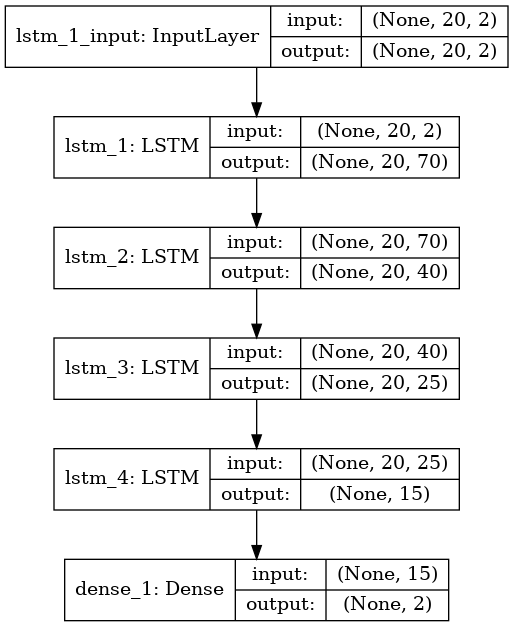
\includegraphics[width=0.67\textwidth]{ figures/net/REC_complex_mod.png}
			\caption{Estructura de LSTM-4 para imágenes modeladas.}
			\label{fig.rec_complex_mod}
		\end{center}
\end{figure}
\vspace{-10pt}
Esta nueva red está compuesta por 4 capas \acrshort{lstm} de 70, 40, 25 y 15 neuronas respectivamente, cuya entrada son las 20 posiciones conocidas y la salida la posición futura estimada.\\
\indent Para llegar a definir la nueva estructura de red se han explorado dos vías: el aumento de neuronas y el de capas, que serán explicados a continuación. Además, se presentan los resultados obtenidos para cada una de las dinámicas consideradas.
\subsection{Aumento de neuronas}
Una vía para la mejora de la red recurrente en las imágenes modeladas es el aumento de neuronas manteniendo una única capa. En este sentido, se duplica el número de neuronas, pasando de las 25 provistas para la red \textit{LSTM-1} a un total de 50. Con esta nueva red, utilizando el conjunto de 100000 muestras que sigue la dinámica sinusoidal con 4~\acrshort{dof}, se obtienen los resultados de la Figura~\ref{fig.units_rec_sin_var2_100000}.

\begin{figure}[H]
		\begin{center}
			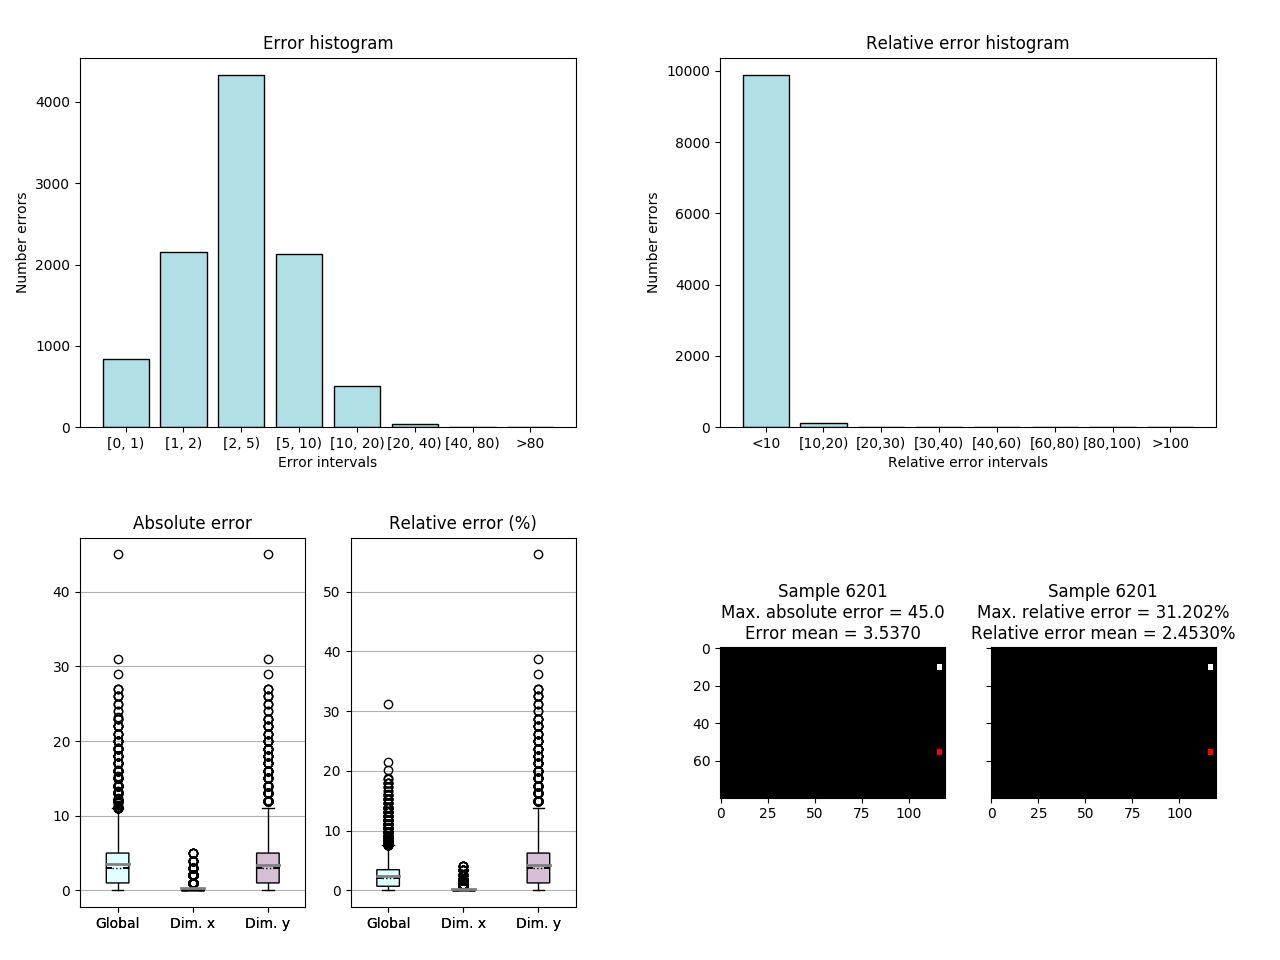
\includegraphics[width=0.8\textwidth]{ figures/test_mod/REC/complex/units_sin_var2_100000.png}
			\caption{Resultados de \acrshort{lstm} de 50 neuronas con dinámica sinusoidal de 4 \acrshort{dof}~(10000 muestras de \textit{test}).}
			\label{fig.units_rec_sin_var2_100000}
		\end{center}
\end{figure}
\vspace{-10pt}

Al comparar los resultados con los equivalentes para la red con menor número de neuronas, en la Figura ~\ref{fig.rec_sin_var2_100000}, se observa una mejora en promedio del error relativo. Este hecho parece corroborar la idea de que la poca capacidad predictiva de la red \textit{LSTM-1}, bajo estas circunstancias, es consecuencia de su simplicidad. Sin embargo, esta mejora no es suficiente para lograr una red que sea capaz de predecir en el caso más complejo.

\subsection{Aumento de capas} \label{ap.capas_mod}
La segunda vía a explorar en la mejora de la red \textit{LSTM-1} es el aumento de del número de capas. En este sentido, se comienza con el aumento de una única capa, que ya proporciona unos datos mucho mejores que los expuestos anteriormente. Este hecho hace ver que esta mecánica es más efectiva que el aumento de neuronas, y reafirma la idea de que una red más compleja captará mejor las distintas relaciones.\\

Con la idea de que el aumento del número de capas es la estrategia más efectiva, se debe establecer el límite de capas a añadir. Para ello se realiza un estudio en el que se aumenta de forma gradual el número de capas, disminuyendo de la misma forma el número de neuronas en cada una de ellas. En la Figura~\ref{fig.capas_mod} se muestra un gráfico en el que se representa la evolución del valor del error relativo, en términos de media y máximo, a medida que se aumentan las capas. Para la elaboración de esta tabla se ha utilizado el mismo conjunto que en el aumento de neuronas, 100000 muestras de sinusoidal con todos sus~\acrshort{dof}.

\begin{figure}[H]
		\begin{center}
			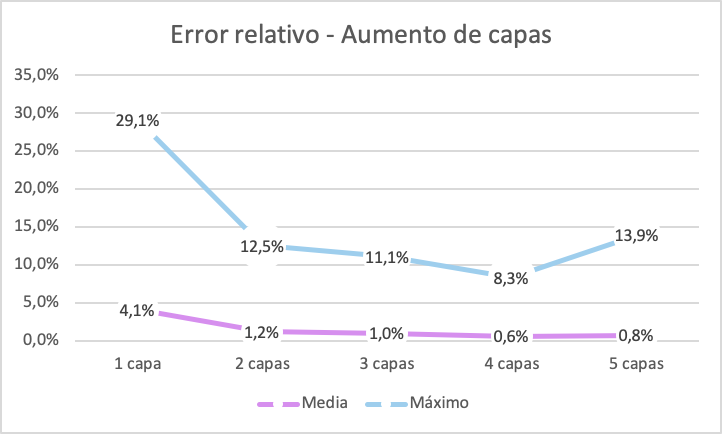
\includegraphics[width=0.7\textwidth]{ figures/test_mod/REC/complex/capas_mod.png}
			\caption{Comparación del error relativo al aumentar el número de capas \acrshort{lstm}~(Sinusoidal, 4~\acrshort{dof}, 10000 muestras de \textit{test}).}
			\label{fig.capas_mod}
		\end{center}
\end{figure}
\vspace{-10pt}

En esta gráfica se puede comprobar que los resultados mejoran a medida que se añaden más capas, hasta llegar a 4 capas. Cuando se emplean 5 capas el error vuelve a subir, empeorando los resultados, lo que hace que se opte por definir la estructura con 4 capas \acrshort{lstm}.

\subsection{Predicción con dinámicas lineales}
En la Figura~\ref{fig.complex_rec_lin_var_100000} se muestran los resultados obtenidos para la dinámica lineal de 2~\acrshort{dof} con esta nueva estructura de red.

\begin{figure}[H]
		\begin{center}
			\includegraphics[width=0.8\textwidth]{ figures/test_mod/REC/complex/linear_var_100000.png}
			\caption{Resultados de LSTM-4 con dinámica lineal de 2 \acrshort{dof}~(10000 muestras de \textit{test}).} 
			\label{fig.complex_rec_lin_var_100000}
		\end{center}
\end{figure}
\vspace{-10pt}
Los resultados obtenidos son muy similares a los de la estructura \acrshort{lstm} con una única capa y 10000 muestras. Este hecho hace concluir que, aunque los resultados son muy buenos, no compensa el aumento del coste computacional pues no se obtiene una mejora significativa.

\subsection{Predicción con dinámicas parabólicas}
Para esta dinámica, cuyo máximo grado de complejidad se alcanza al tener 3~\acrshort{dof}, los resultados obtenidos al evaluar la estructura de red propuesta se muestran en la Figura~\ref{fig.complex_rec_parab_var1_100000}.

\begin{figure}[H]
		\begin{center}
			\includegraphics[width=0.8\textwidth]{ figures/test_mod/REC/complex/parab_var1_100000.png}
			\caption{Resultados de LSTM-4 con dinámica parabólica de 3 \acrshort{dof}~(10000 muestras de \textit{test}).} 
			\label{fig.complex_rec_parab_var1_100000}
		\end{center}
\end{figure}
\vspace{-10pt}

Al igual que ocurre en el caso anterior, la capacidad de predicción de la red \textit{LSTM-1} ya es buena para esta dinámica con un conjunto de 10000 muestras. Los resultados arrojados al utilizar un conjunto más grande con una estructura más compleja reafirman lo concluido en el caso lineal: no compensa el coste computacional por la mejora.

\subsection{Predicción con dinámicas sinusoidales}
La última dinámica considerada hasta el momento, regida por la función sinusoidal, establece su máxima complejidad en 4~\acrshort{dof}. Los resultados de entrenar y evaluar la nueva red con el \textit{dataset} de 100000 muestras y dichos grados de libertad se muestran en la Figura~\ref{fig.complex_rec_sin_var2_100000}.

\begin{figure}[H]
		\begin{center}
			\includegraphics[width=0.8\textwidth]{ figures/test_mod/REC/complex/layers_sin_var2_100000.png}
			\caption{Resultados de LSTM-4 con dinámica sinusoidal de 4 \acrshort{dof}~(10000 muestras de \textit{test}).} 
			\label{fig.complex_rec_sin_var2_100000}
		\end{center}
\end{figure}
\vspace{-10pt}

En esta última dinámica no se habían conseguido unos resultados demasiado buenos con la estructura \textit{LSTM-1}, había un alto grado de incertidumbre. Con la nueva estructura de red los resultados de la misma mejoran considerablemente, lo que hace que se pueda predecir con mayor certeza. Por tanto, sí que resulta efectivo aumentar la complejidad y, con ello el coste computacional, por una mejora en la capacidad predictiva para la dinámica.

\subsection{Predicción con dinámica combinada}
Tras haber dominado por separado las dinámicas en su grado más complejo, se ha considerado un nuevo conjunto que contiene 33000 ejemplos lineales y parabólicos, y 34000 sinusoidales, con el objetivo de explorar una dinámica combinada. La red se entrena y evalúa con este nuevo conjunto y se obtienen los resultados mostrados en la Figura~\ref{fig.complex_rec_mix_100000}.

\begin{figure}[H]
		\begin{center}
			\includegraphics[width=0.8\textwidth]{ figures/test_mod/REC/complex/mix_100000.png}
			\caption{Resultados de LSTM-4 con dinámica combinada~(10000 muestras de \textit{test}).} 
			\label{fig.complex_rec_mix_100000}
		\end{center}
\end{figure}
\vspace{-10pt}

Los resultados están limitados por los obtenidos para cada dinámica por separado. Al mezclar las muestras en la misma proporción, con algún ejemplo más de la sinusoidal, no se espera mejorar los resultados de la que peor predice. De esta forma, aunque se comete mayor error respecto al caso sinusoidal, se consigue mantener la capacidad de predicción en términos generales.

\subsection{Predicción a largo plazo} 
El último experimento propuesto en cuanto a la predicción de las imágenes modeladas consiste en el análisis de la repercusión del horizonte temporal en la calidad de la predicción. Para ello se ha utilizado el conjunto de la dinámica combinada con 100000 muestras incrementando el valor del \textit{gap} gradualmente. En la Figura~\ref{fig.gap} se muestra la evolución del error relativo obtenido, en términos de media y máximo, a medida que se modifica este parámetro.

\begin{figure}[H]
		\begin{center}
			\includegraphics[width=0.7\textwidth]{ figures/test_mod/REC/complex/largoplazo.png}
			\caption{Comparación del error relativo al aumentar el \textit{gap}~(Combinada, 10000 muestras de \textit{test})}
			\label{fig.gap}
		\end{center}
\end{figure}
\vspace{-10pt}

A la vista de estos resultados queda patente el hecho de que poner la vista en una posición más lejana en el tiempo complica la tarea de predicción de la red. A medida que se aumenta la separación temporal entre el último elemento conocido y el que se quiere estimar la relación entre ambas se va difuminando, perdiendo la capacidad de predicción progresivamente. Sin embargo, esta pérdida se realiza siempre en umbrales admisibles: en una imagen de 640x480, por ejemplo, se obtienen 14 píxeles de media de error a 30 fotogramas (1.7\%) y 24 a 50 fotogramas (3\%).

\subsection{Resumen de resultados}
En la Tabla~\ref{tab.lstm4} se muestra el resumen de los resultados obtenidos en las distintas dinámicas consideradas para la red \textit{LSTM-4}.
\begin{table}[H]
	\centering
	\begin{tabular}{{|l|c|c|}}
		\hline
		\multicolumn{2}{|c|}{\textbf{Dinámica}} & \textbf{LSTM-4}\\ \hline 
		\multicolumn{1}{|c|}{Lineal}
        &2~\acrshort{dof} & \cellcolor{darkgreen}0.12\%\\ 
        \hline
        \multicolumn{1}{|c|}{Parabólica}
        &3~\acrshort{dof} & \cellcolor{darkgreen}0.5\%\\ 
        \hline
        \multicolumn{1}{|c|}{Sinusoidal}
        &4~\acrshort{dof} & \cellcolor{greenyellow}0.61\%\\
        \hline
        \multicolumn{2}{|c|}{Combinada} & \cellcolor{greenyellow}0.81\%\\ \hline 
	\end{tabular}
	\caption{Promedio del error relativo en \textit{test} al evaluar la red LSTM-4 con imágenes modeladas y distintas dinámicas (10000 muestras de \textit{test}).}
	\label{tab.lstm4}
\end{table}

Como anteriormente,se han evaluado todas las redes con un conjunto de 10000 muestras para que la comparación entre ellas sea equitativa.

\section{Comparativa global} \label{sec.comp_mod}
Tras realizar los experimentos con imágenes modeladas se obtiene un conjunto de redes entrenadas para las distintas dinámicas. Con el objetivo de compararlas de una forma rápida, se ha elaborado la Tabla~\ref{tab.comp_mod}. Esta tabla sigue el mismo código de colores especificado en el Apartado~\ref{ap.resumen_RNNmlp}, añadiendo el gris para aquellos experimentos que no han sido considerados. Además, el valor numérico asociado, promedio del error relativo, ilustra de una forma cuantitativa las prestaciones obtenidas, aunque no es la única figura de mérito utilizada para la asignación del color en la celda. También se han evaluado todas las redes con un conjunto de 10000 muestras para una comparación equitativa.

\begin{table}[H]
	\centering
	\begin{tabular}{{|l|c|c|c|c|}}
		\hline
		\multicolumn{2}{|c|}{\textbf{Dinámica}} & \textbf{\acrshort{mlp}} & \textbf{LSTM-1} & \textbf{LSTM-4}\\ \hline 
		\multirow{2}{*}{Lineal}
		&1~\acrshort{dof} & \cellcolor{darkgreen}0.21\% & \cellcolor{darkgreen}0.16\% & \cellcolor{gray!30}\\
		\cline{2-5}
        &2~\acrshort{dof} & \cellcolor{darkgreen}0.31\% & \cellcolor{darkgreen}0.25\% & \cellcolor{darkgreen}0.12\% \\ 
        \hline
        \multirow{3}{*}{Parabólica}
        &1~\acrshort{dof} & \cellcolor{darkgreen}0.28\% & \cellcolor{darkgreen}0.12\% & \cellcolor{gray!30}\\
		\cline{2-5}
        &2~\acrshort{dof} & \cellcolor{darkgreen}0.42\% & \cellcolor{darkgreen}0.35\% & \cellcolor{gray!30}\\
        \cline{2-5}
        &3~\acrshort{dof} & \cellcolor{darkgreen}0.65\%& \cellcolor{darkgreen}0.58\%& \cellcolor{darkgreen}0.6\%\\ 
        \hline
        \multirow{4}{*}{Sinusoidal}
        &1~\acrshort{dof} & \cellcolor{darkgreen}0.54\% & \cellcolor{darkgreen}0.42\% & \cellcolor{gray!30} \\
        \cline{2-5}
        &2~\acrshort{dof} & \cellcolor{myorange}3.89\% & \cellcolor{greenyellow}0.89\% & \cellcolor{gray!30} \\
        \cline{2-5}
        &3~\acrshort{dof} & \cellcolor{gray!30} & \cellcolor{greenyellow}0.84\% & \cellcolor{gray!30} \\
        \cline{2-5}
        &4~\acrshort{dof} & \cellcolor{gray!30} & \cellcolor{myorange} 4.09\%& \cellcolor{greenyellow}0.61\%\\ 
        \hline
        \multicolumn{2}{|c|}{Combinada} & \cellcolor{gray!30} & \cellcolor{gray!30} & \cellcolor{greenyellow}0.81\%\\ \hline 
	\end{tabular}
	\caption{Comparativa del promedio de error relativo en las distintas redes para imágenes modeladas con las distintas dinámicas (10000 muestras de \textit{test}).}
	\label{tab.comp_mod}
\end{table}

Se puede observar que la red que mejores resultados aporta es la \textit{LSTM-4}, que es capaz de realizar una predicción razonable en todas las dinámicas consideradas. Además, se refleja que el uso de la recurrencia aporta una mejora en la calidad de la predicción y que el aumento de capas recurrentes hace que se lleguen a dominar todas las dinámicas en su grado más complejo.

\lhead[]{CAPÍTULO \thechapter. PREDICCIÓN DE IMÁGENES CRUDAS}
\chapter{Predicción con imágenes crudas}\label{cap.redes3dcrud}

En este capíıtulo se presentan los estudios realizados para la predicción en imágenes crudas, con el objetivo de explorar distintas estructuras neuronales para abordar el problema. Al igual que en las imágenes modeladas, se pone el foco en el análisis de las redes recurrentes y, más concretamente, de aquéllas que mantienen la relación espacio-temporal.\\

Para las imágenes crudas, la tarea no se aborda como un problema clásico de regresión. Se quiere predecir una imagen en la que todos los píxeles toman un valor nulo salvo uno de ellos, considerado como activo. Esta naturaleza de las imágenes a predecir hace que se pueda afrontar el problema como una tarea de clasificación binaria donde la salida se corresponde con un vector de longitud $h \times w$, con la codificación de la clase en cada píxel. Para volver a obtener una imagen, según se explicó en la Sección~\ref{sec.eval}, se redimensiona el vector de salida a una matriz $h \times w$ que se pasa a una imagen en escala de grises con 8 bits por píxel.\\

La características que siguen todos los conjuntos de datos utilizados para este estudio, en lo que a \textit{n}\_\textit{points}, \textit{gap} y división en subconjuntos se refiere, son las mismas que las establecidas en el Capítulo~\ref{cap.redes3dmod} para imágenes modeladas. Además, cada una de las imágenes que forma una muestra tienen un tamaño de $80 \times 120$ píxeles.\\

A continuación se realiza el recorrido por las  estructuras neuronales entrenadas con imágenes crudas, mostrando los resultados obtenidos y las conclusiones que originan nuevas vías de investigación para la mejora de los mismos.


\section{Arquitectura no recurrente: Red convolucional} \label{sec.raw_norec_cnn}

Para abordar el estudio de la predicción en imágenes crudas con una arquitectura sin recurrencia se utiliza una \acrshort{cnn}, introducida en el Apartado~\ref{ap.cnn}. En la Figura~\ref{fig.cnn_raw} se presenta la estructura escogida para abordar la tarea de predicción con imágenes crudas. En este caso, la entrada a la red es una secuencia con 20 imágenes de tamaño $h \times w$, que alimenta dos capas consecutivas de convolución seguidas de una de reducción o \textit{pooling}. A la salida se obtiene un vector de longitud $h \times w$ que será redimensionado posteriormente para obtener una imagen.
\begin{figure}[H]
		\begin{center}
			\includegraphics[width=0.8\textwidth]{ figures/net/NOREC_simple_raw.png}
			\caption{Estructura de \acrshort{cnn} para imágenes crudas.}
			\label{fig.cnn_raw}
		\end{center}
\end{figure}
\vspace{-10pt}

Una vez definida la red, se realizan experimentos con conjuntos de secuencias de imágenes crudas donde la complejidad de movimiento del píxel activo va aumentando de forma progresiva, tanto con el tipo de dinámica como en el número de grados de libertad para la misma dinámica.

\subsection{Influencia del número de muestras}
Con el objetivo de analizar la influencia que el número de muestras tiene en el aprendizaje de la red, se ha desarrollado un experimento en el que dicho número aumenta de forma progresiva, entrenando la estructura descrita anteriormente. Se han empleado muestras cuyos píxeles siguen una dinámica lineal de un único \acrshort{dof}, evaluando todas las redes con un mismo conjunto de \textit{test} de 1000 muestras. Los resultados se muestran en la gráfica de la Figura~\ref{fig.n_muestras}.

\begin{figure}[H]
		\begin{center}
			\includegraphics[width=0.7\textwidth]{ figures/test_raw/NOREC/n_muestras.png}
			\caption{Comparación del error relativo al aumentar el número de muestras de entrenamiento con \acrshort{cnn}~(Lineal, 1~\acrshort{dof}, 1000).}
			\label{fig.n_muestras}
		\end{center}
\end{figure}
\vspace{-10pt}


En el gráfico se puede comprobar cómo aumentar el número de muestras de entrenamiento produce un efecto positivo en las prestaciones de la red hasta un límite, a partir del cuál las prestaciones se mantienen. Este valor límite en el número de muestras dependerá de la complejidad de la dinámica  dinámica que rige el movimiento. Para las dinámicas más sencillas se necesitará un número menor de muestras de entrenamiento que para las más complejas. Mediante el el uso de un número adecuado de muestras en el entrenamiento se evita que no haya suficientes secuencias para que la red sea capaz de aprender y, por otro lado, que la red vea todos los ejemplos de la dinámica y memorice las relaciones entre la entrada y la salida, evitando la generalización.

\subsection{Predicción con dinámicas lineales}
Para abordar la predicción de fotogramas donde se representan objetos que siguen una dinámica lineal, se utiliza un \textit{dataset} compuesto por 10000 muestras. Este conjunto de datos se divide en tres, de tal forma que 8000 muestras se utilizan para el entrenamiento, 1000 para la validación y 1000 para el \textit{test}.\\

En la Figura~\ref{fig.raw_norec_lin_fix_10000} se muestran los resultados obtenidos al evaluar la \acrshort{cnn} propuesta entrenada con dicho conjunto cuando se considera un único \acrshort{dof}, la pendiente de la trayectoria del píxel activo. Se observa que las prestaciones de la red son buenas, pues se consigue un error relativo muy reducido en términos de media y máximo.

\begin{figure}[H]
		\begin{center}
			\includegraphics[width=0.8\textwidth]{ figures/test_raw/NOREC/linear_fix_10000.png}
			\caption{Resultados de \acrshort{cnn} con dinámica lineal de 1 \acrshort{dof}~(1000 muestras de \textit{test}).}
			\label{fig.raw_norec_lin_fix_10000}
		\end{center}
\end{figure}
\vspace{-10pt}


Al aumentar el grado de complejidad de la dinámica añadiendo un nuevo \acrshort{dof}, la posición vertical en la imagen desde la que el píxel activo comienza su movimiento recto. Los resultados obtenidos bajo esta nueva premisa, utilizando el mismo número de muestras y distribución de los subconjuntos que en el caso anterior, se muestran en la Figura~\ref{fig.raw_norec_lin_var_10000}.

\begin{figure}[H]
		\begin{center}
			\includegraphics[width=0.8\textwidth]{ figures/test_raw/NOREC/linear_var_10000.png}
			\caption{Resultados de \acrshort{cnn} con dinámica lineal de 2 \acrshort{dof}~(1000 muestras de \textit{test}).}
			\label{fig.raw_norec_lin_var_10000}
		\end{center}
\end{figure}
\vspace{-10pt}

En esta ocasión, el resultado obtenido muestra un deterioro de las prestaciones de la red. Al tratar directamente con todos los píxeles de la imagen y no reducir la información a un par de valores (\textit{x}, \textit{y}), como en el caso de las modeladas, el número de parámetros que utiliza la red se ha elevado enormemente. Este hecho hace que, para el caso que se está tratando (dinámica lineal con 2\acrshort{dof}, la cantidad de ejemplos que se introducen a la red durante el entrenamiento pueda no ser suficiente. Para solucionar este problema  se decide aumentar el número de muestras del conjunto en un factor de 10, pasando de los 10000 ejemplos a 100000. La división en los tres subconjuntos se realiza con una asignación de 80000 para entrenamiento, 10000 para validación y 10000 para \textit{test}. Con este incremento en el número de muestras se vuelve a entrenar y a evaluar la misma estructura \acrshort{cnn}, obteniendo los resultados de la Figura~\ref{fig.raw_norec_lin_var_100000}.

\begin{figure}[H]
		\begin{center}
			\includegraphics[width=0.8\textwidth]{ figures/test_raw/NOREC/linear_var_100000.png}
			\caption{Resultados de \acrshort{cnn} con dinámica lineal de 2 \acrshort{dof}~(10000 muestras de \textit{test}).}
			\label{fig.raw_norec_lin_var_100000}
		\end{center}
\end{figure}
\vspace{-10pt}

Se observa que con el aumento en el número de muestras de entrenamiento se mejoran las prestaciones de la red en términos de promedio del error relativo, pero siguen existiendo algunos \textit{outliers}, valores atípicos que perjudican a la predicción y no permiten obtener resultados óptimos.

\subsection{Predicción con dinámicas parabólicas}
Para abordar la predicción de fotogramas donde se representan objetos que siguen una dinámica parabólica se utiliza un \textit{dataset} compuesto por 100000 muestras. Este conjunto de datos queda dividido en tres subconjuntos, utilizando 80000 muestras para el entrenamiento, 10000 para la validación y 10000 para el \textit{test}.\\

Se comienza el estudio con el caso más sencillo de la dinámica, un único \acrshort{dof}~(valor de \textit{a}). Los resultados obtenidos se reflejan en la Figura~\ref{fig.raw_norec_par_fix_100000}. Las prestaciones de la red son muy buenas, se obtienen valores muy bajos de error y el número de \textit{outliers} es también muy reducido.

\begin{figure}[H]
		\begin{center}
			\includegraphics[width=0.8\textwidth]{ figures/test_raw/NOREC/parabolic_fix_100000.png}
			\caption{Resultados de \acrshort{cnn} con dinámica parabólica de 1 \acrshort{dof}~(10000 muestras de \textit{test}).}
			\label{fig.raw_norec_par_fix_100000}
		\end{center}
\end{figure}
\vspace{-10pt}

Se aumenta la complejidad de la dinámica con un nuevo \acrshort{dof}, la posición vertical inicial del píxel en la imagen (valor de \textit{c}), manteniendo el número de muestras y la distribución de los subconjuntos  del caso anterior. Los resultados obtenidos sobre la red entrenada con este conjunto se muestran en la Figura~\ref{fig.raw_norec_par_var_100000}. En esta ocasión, al contrario que ocurría en la dinámica lineal, el aumento de la complejidad, aunque empeora los resultados, no provoca que la red pierda su capacidad predictiva.\\

Finalmente, dentro de esta dinámica se establecen 3 \acrshort{dof}. Se utiliza el mismo número de muestras por subconjunto que en los casos anteriores, obteniendo los resultados de la Figura~\ref{fig.raw_norec_par_var1_100000}. En ella se refleja que los valores de error son elevados, se produce un gran número de \textit{outliers} y la caja de los \textit{boxplot} se separa ligeramente del valor nulo. Con todo esto, las prestaciones de la red se reducen respecto a los casos anteriores, empeorando la capacidad predictiva de la red.

\begin{figure}[H]
		\begin{center}
			\includegraphics[width=0.8\textwidth]{ figures/test_raw/NOREC/parabolic_var_100000.png}
			\caption{Resultados de \acrshort{cnn} con dinámica parabólica de 2 \acrshort{dof}~(10000 muestras de \textit{test}).}
			\label{fig.raw_norec_par_var_100000}
		\end{center}
\end{figure}
\vspace{-30pt}
\begin{figure}[H]
		\begin{center}
			\includegraphics[width=0.8\textwidth]{ figures/test_raw/NOREC/parabolic_var1_100000.png}
			\caption{Resultados de \acrshort{cnn} con dinámica parabólica de 3 \acrshort{dof}~(10000 muestras de \textit{test}).}
			\label{fig.raw_norec_par_var1_100000}
		\end{center}
\end{figure}
\vspace{-10pt}

\subsection{Predicción con dinámicas sinusoidales}
Para abordar la predicción de fotogramas que representan objetos que siguen una dinámica sinusoidal, se utiliza un \textit{dataset} compuesto por 100000 muestras. Sobre el total de muestras establecido se realiza una división de tal forma que 80000 muestras se utilizan para el entrenamiento, 10000 para la validación y 10000 para el \textit{test}.\\

Se comienza con la variante más sencilla de esta dinámica, que deja como parámetro aleatorio la frecuencia de la sinusoide, 1~\acrshort{dof}. En la Figura~\ref{fig.raw_norec_sin_fix_100000} se muestran los resultados obtenidos, donde se puede comprobar que la red tiene muy buenas prestaciones para este caso.
\begin{figure}[H]
		\begin{center}
			\includegraphics[width=0.8\textwidth]{ figures/test_raw/NOREC/sin_fix_100000.png}
			\caption{Resultados de \acrshort{cnn} con dinámica sinusoidal de 1 \acrshort{dof}~(10000 muestras de \textit{test}).}
			\label{fig.raw_norec_sin_fix_100000}
		\end{center}
\end{figure}
\vspace{-10pt}

A continuación, se permite que la posición vertical inicial del píxel en la imagen tome también un valor aleatorio, estableciendo la dinámica con 2~\acrshort{dof}. Tras entrenar y evaluar la red propuesta con los subconjuntos correspondientes, cuyas características son las mismas que en casos anteriores, se obtienen los resultados de la Figura~\ref{fig.raw_norec_sin_var_100000}. Estos valores reflejan un deterioro de las prestaciones de la red por la complejidad de la dinámica. Los valores de error han aumentado considerablemente, especialmente el máximo, y se obtiene un número de \textit{outliers} mucho mayor que en el caso más sencillo. Con estos resultados, se establece el límite de predicción con la \acrshort{cnn} propuesta para dinámicas sinusoidales en un único \acrshort{dof}.

\begin{figure}[H]
		\begin{center}
			\includegraphics[width=0.8\textwidth]{ figures/test_raw/NOREC/sin_var_100000.png}
			\caption{Resultados de \acrshort{cnn} con dinámica sinusoidal de 2 \acrshort{dof}~(10000 muestras de \textit{test}).}
			\label{fig.raw_norec_sin_var_100000}
		\end{center}
\end{figure}
\vspace{-10pt}

\subsection{Resumen de resultados}

En la Tabla~\ref{tab.cnn} se muestra un resumen de los resultados alcanzados en cada dinámica con imágenes de píxeles 2D. Para la interpretación de esta tabla se ha establecido un código de cuatro colores que reflejan, de mejor a peor, los resultados obtenidos en cada experimento. La secuencia de colores utilizada comienza con el verde oscuro para resultados muy buenos, pasando por el verde claro y el naranja, para terminar con el rojo, que indica malos resultados. Para  realizar una comparación equitativa, se ha vuelto a evaluar la dinámica lineal de 1~\acrshort{dof} con 10000, proporcionando un promedio de error relativo de 0.07\%. 

\begin{table}[H]
	\centering
	\begin{tabular}{{|l|c|c|}}
		\hline
		\multicolumn{2}{|c|}{\textbf{Dinámica}} & \textbf{\acrshort{cnn}}\\ \hline 
		\multirow{2}{*}{Lineal}
		&1~\acrshort{dof} & \cellcolor{darkgreen}{0.07\%}\\
		\cline{2-3}
        &2~\acrshort{dof} & \cellcolor{greenyellow}{0.39\%}\\
        \hline
        \multirow{3}{*}{Parabólica}
        &1~\acrshort{dof} & \cellcolor{darkgreen}0.01\%\\
        \cline{2-3}
        &2~\acrshort{dof} & \cellcolor{darkgreen}0.07\%\\
        \cline{2-3}
        &3~\acrshort{dof} & \cellcolor{red}4.40\%\\ 
        \hline
        \multirow{2}{*}{Sinusoidal}
        &1~\acrshort{dof} & \cellcolor{darkgreen}0.003\%\\
        \cline{2-3}
        &2~\acrshort{dof} & \cellcolor{myorange}1.12\%\\
        \hline
	\end{tabular}
	\caption{Promedio del error relativo en \textit{test} al evaluar la \acrshort{cnn} con imágenes modeladas y distintas dinámicas (10000 muestras de \textit{test}).}
	\label{tab.cnn}
\end{table}

\section{Arquitectura recurrente: Convolucional + LSTM}
Una vía de investigación en cuanto al efecto de introducir la recurrencia en la predicción de imágenes es combinar una capa convolucional, que capte las relaciones espaciales, con una capa \acrshort{lstm} posterior, para las relaciones temporales. La estructura propuesta se muestra en la Figura~\ref{fig.cnn_lstm_raw}.

\begin{figure}[H]
		\begin{center}
			\includegraphics[width=0.9\textwidth]{ figures/net/REC_simple_raw.png}
			\caption{Estructura de \acrshort{cnn}+\acrshort{lstm} para imágenes crudas.}
			\label{fig.cnn_lstm_raw}
		\end{center}
\end{figure}
\vspace{-10pt}

La red consta de una capa convolucional de 32 neuronas seguida de su correspondiente capa de reducción. Tras la estructura propia de las \acrshort{cnn} se añade una capa para \textit{flatten} para obtener un vector de una dimensión que será la entrada a la única capa \acrshort{lstm} con 25 neuronas.

\subsection{Predicción con dinámicas lineales}
Para estudiar el efecto de la recurrencia con la arquitectura de red propuesta, se comienza con el caso más sencillo de todos: dinámica lineal de pendiente nula y con posición vertical inicial del píxel fija. El conjunto consta de  1000 muestras, de las cuales 800 son para entrenamiento, 100 para validación y otras 100 para \textit{test}. Al evaluar la red \acrshort{cnn} propuesta en la Sección~\ref{sec.raw_norec_cnn} con el mismo conjunto se obtiene un error completamente nulo, según se muestra en la Figura~\ref{fig.raw_norec_urm_fix_1000}; sin embargo, al introducir la capa \acrshort{lstm}, la red pierde toda su capacidad predictiva pasando de un 100\% de acierto a un 70\%, según se muestra en la Figura~\ref{fig.raw_rec_urm_fix_1000}.

\begin{figure}[H]
		\begin{center}
			\includegraphics[width=0.8\textwidth]{ figures/test_raw/NOREC/URM_fix_1000.png}
			\caption{Resultados de \acrshort{cnn} con dinámica lineal, pendiente nula y altura fija~(100 muestras de \textit{test}).} 
			\label{fig.raw_norec_urm_fix_1000}
		\end{center}
\end{figure}
\vspace{-10pt}

\begin{figure}[H]
		\begin{center}
			\includegraphics[width=0.8\textwidth]{ figures/test_raw/REC/CONV+LSTM/URM_fix_1000.png}
			\caption{Resultados de \acrshort{cnn}+\acrshort{lstm} con dinámica lineal, pendiente nula y altura fija~(100 muestras de \textit{test}).} 
			\label{fig.raw_rec_urm_fix_1000}
		\end{center}
\end{figure}
\vspace{-10pt}

Con estos resultados se puede concluir que analizar las relaciones temporales de forma independiente a las espaciales no parece una buena estrategia.

\subsection{Extensión gradual del punto activo}
Una de las posibles causas de que esta estrategia de combinar una \acrshort{cnn} con una \acrshort{lstm} no funcione correctamente es que se están empleando  imágenes con un único píxel activo, complicando a la red la tarea de encontrar correlaciones espaciales. Para analizar este hecho se decide ampliar la zona activa de la imagen, reduciendo de forma gradual el nivel de intensidad de los píxeles alrededor del píxel activo, haciendo uso de una función gaussiana isotrópica. En la Figura~\ref{fig.pixel} se muestra tanto el píxel utilizado hasta ahora, que denominaremos píxel discreto, como el resultado de convolucionar un filtro gaussiano con centro en dicho píxel y entorno activo 5x5.

\begin{figure}[H]
		\begin{center}
			\subfigure[]{\includegraphics[width=0.5\textwidth]{ figures/pixel_discreto.png}}
	        \subfigure[]{\frame{\includegraphics[width=0.5\textwidth]{ figures/pixel_gaussiano.png}}}
	        \caption{Ejemplos de píxel: (a)~Discreto y (b)~Expandido.}
			\label{fig.pixel}
		\end{center}
\end{figure}
\vspace{-10pt}

La intuición subyacente es que, al extender el píxel, los algoritmos que hacen uso de correlación espacial pueden tener valores gradualmente crecientes al acercarse a una correlación máxima, y tal vez durante el aprendizaje se vean ayudados a converger hacia ese máximo. Con un píxel discreto las correlaciones entre los píxeles de la imagen son todas nulas excepto en el máximo, lo que no ayuda a los algoritmos de aprendizaje (que se suelen apoyar en gradientes) a encontrarlo: en las cercanías del píxel activo las correlaciones valen igual que si se está lejos del mismo.\\

Para analizar la repercusión que tiene en evaluación el aprendizaje con extensión del píxel, se emplea el mismo conjunto de dinámica lineal utilizado anteriormente, aplicándole a las imágenes una convolución con el filtro gaussiano antes de su entrada a la red. En la Figura~\ref{fig.raw_rec_urm_fix_1000_gauss} se muestran los resultados de este nuevo experimento.

\begin{figure}[H]
		\begin{center}
			\includegraphics[width=0.8\textwidth]{ figures/test_raw/REC/CONV+LSTM/URM_fix_1000_Gauss.png}
			\caption{Resultados de \acrshort{cnn}+\acrshort{lstm} con píxel extendido en dinámica lineal, pendiente nula y altura fija~(100 muestras de \textit{test}).} 
			\label{fig.raw_rec_urm_fix_1000_gauss}
		\end{center}
\end{figure}
\vspace{-10pt}

Aunque los resultados han mejorado en términos de valores medios, la red continúa sin ser capaz de predecir correctamente. Además, la caja del \textit{boxplot} se ha visto desplazada hacia arriba, dejando los valores más bajos de error como \textit{outliers} de los resultados. Con este análisis se concluye que, por un lado, la estrategia de combinar por separado ambas relaciones no es adecuada, y por el otro, extender el píxel para facilitar el análisis de las correlaciones espaciales en la imagen no es una mejora.

\subsection{Resumen de resultados}
A modo de resumen, la Tabla~\ref{tab.conv+lstm} se muestran los resultados de los experimentos relacionados con la estructura que combina una capa convolucional con una \acrshort{lstm} posterior a modo de resumen.

\begin{table}[H]
	\centering
	\begin{tabular}{{|l|c|c|c|}}
		\hline
		\multicolumn{2}{|c|}{\textbf{Dinámica}} & \textbf{\acrshort{cnn}} & \textbf{\acrshort{cnn}+\acrshort{lstm}}\\ \hline 
		\multirow{2}{*}{Lineal}
		&Discreto & \cellcolor{darkgreen}{0.0\%} & \cellcolor{red}{29.6\%}\\
		\cline{2-3}
        &Extendido & \cellcolor{gray!30} & \cellcolor{red}{21.5\%}\\
        \hline
	\end{tabular}
	\caption{Promedio del error relativo en \textit{test} al evaluar la red \acrshort{cnn}+\acrshort{lstm} con imágenes modeladas y distintas dinámicas (10000 muestras de \textit{test}).}
	\label{tab.conv+lstm}
\end{table}

\section{Arquitectura recurrente: ConvLSTM-1}
Otra vía a explorar, en cuanto al efecto de la recurrencia en la capacidad de predicción de las redes, es el uso de las redes \textit{ConvLSTM} presentadas en el Apartado~\ref{ap.convLSTM}. Para ello, se define la estructura de red de la Figura~\ref{fig.convLSTM1}.

\begin{figure}[H]
		\begin{center}
			\includegraphics[width=0.9\textwidth]{ figures/net/REC_convLSTM_simple.png}
			\caption{Estructura de ConvLSTM-1 para imágenes crudas.}
			\label{fig.convLSTM1}
		\end{center}
\end{figure}
\vspace{-10pt}

Debido a la cantidad de valores en cada una de las secuencias de entrada, 20 imágenes con $80 \times 120$ píxeles, es necesario realizar una reducción de la dimensionalidad para que la máquina sea capaz de procesar todos los valores. Para ello se introduce tras la entrada de la red dos capas convolucionales, de 32 neuronas cada una, seguidas de su capa de \textit{pooling}, que reducen la cantidad de valores a procesar. Posteriormente, se utiliza una única capa \textit{ConvLSTM} de 5 neuronas que será la encargada de analizar las correlaciones espacio-temporales de las entradas.\\

Con la estructura de red definida se realizan experimentos sobre todas las dinámicas propuestas, aumentando de forma progresiva la complejidad de cada una de ellas.

\subsection{Predicción con dinámicas lineales}
Para la predicción en imágenes cuyo píxel se mueve siguiendo una dinámica lineal con un solo \acrshort{dof}, se utiliza el mismo conjunto que en el caso no recurrente: un total del 10000 muestras repartidas en 8000 para entrenar, 1000 para validar y 1000 para evaluar. La Figura~\ref{fig.raw_convlstm1_lin_fix_10000} muestra los resultado obtenidos con dicho conjunto.

\begin{figure}[H]
		\begin{center}
			\includegraphics[width=0.8\textwidth]{ figures/test_raw/REC/ConvLSTM_simple/linear_fix_10000.png}
			\caption{Resultados de ConvLSTM-1 con dinámica lineal de 1 \acrshort{dof}~(1000 muestras de \textit{test}).}
			\label{fig.raw_convlstm1_lin_fix_10000}
		\end{center}
\end{figure}
\vspace{-10pt}

Los resultados obtenidos para esta dinámica con un \acrshort{dof} son similares a los del caso no recurrente, proporcionando una muy buena capacidad predictiva para ambos tipos de redes. Estos resultados indican que la nueva estructura de red recurrente no deteriora las prestaciones de la estructura no recurrente, como sí ocurría con la estructura combinada de \acrshort{cnn} y \acrshort{lstm} posterior.\\

Siguiendo el procedimiento establecido hasta el momento, se aumenta la complejidad de la dinámica estableciendo 2 \acrshort{dof}, y se vuelve a entrenar la estructura neuronal propuesta. En este caso se utiliza un conjunto de 100000 muestras, distribuidas en 80000 de entrenamiento, 10000 de validación y 10000 de \textit{test}. En la Figura~\ref{fig.raw_convlstm1_lin_var_100000} se muestran las prestaciones de dicha red bajo las condiciones mencionadas.

\begin{figure}[H]
		\begin{center}
			\includegraphics[width=0.8\textwidth]{ figures/test_raw/REC/ConvLSTM_simple/linear_var_100000.png}
			\caption{Resultados de ConvLSTM-1 con dinámica lineal de 2 \acrshort{dof}~(10000 muestras de \textit{test}).}
			\label{fig.raw_convlstm1_lin_var_100000}
		\end{center}
\end{figure}
\vspace{-10pt}

Al comparar los resultados con los de la red convolucional, representados en la Figura~\ref{fig.raw_norec_lin_var_100000}, se observa una gran mejoría de la estructura recurrente~(ConvLSTM-1) respecto a la no recurrente~(\acrshort{cnn}). Se reducen los valores de error relativo tanto en media como en máximo, y la cantidad de \textit{outliers} es también menor. Este hecho refuerza la conclusión extraída con las imágenes modeladas de que la recurrencia, bien aplicada, mejora las prestaciones de las redes como predictores visuales.

\subsection{Predicción con dinámicas parabólicas}
En el caso de imágenes cuyo píxel activo sigue una la dinámica parabólica, se emplea un conjunto con 100000 ejemplos, de los que 80000 se emplearán para entrenar, 10000 para validar y otros 10000 para evaluar. En la Tabla~\ref{tab.cnn_convlstm_parab} se muestra la comparación del error relativo obtenido, tanto máximo como medio, con la red sin recurrencia, la \acrshort{cnn}, y con la red recurrente \textit{ConvLSTM-1}. En dicha tabla se reafirma el hecho de que introducir de manera adecuada la recurrencia en la estructura de la red conduce a una mejora en las prestaciones.

\begin{table}[H]
	\centering
	\begin{tabular}{{l|c|c|c|c|}}
		\cline{2-5}
		& \multicolumn{2}{|c|}{\textbf{\acrshort{cnn}}} & \multicolumn{2}{|c|}{\textbf{ConvLSTM-1}} \\
		\hline
		\multicolumn{1}{|l|}{\textbf{\acrshort{dof}}} & \textbf{\textit{Max.}} & \textbf{\textit{Mean}} & \textbf{\textit{Max.}} & \textbf{\textit{Mean}}\\
		\hline 
		\multicolumn{1}{|l|}{\textbf{1~(\textit{a})}} &  0.7\% &  0.01\% & 0.7\% & 0.01\%\\ \hline
		\multicolumn{1}{|l|}{\textbf{2~(\textit{c})}} &  8.3\% &  0.07\% & 4.9\% & 0.03\%\\ \hline
		\multicolumn{1}{|l|}{\textbf{3~(\textit{b})}} &  54.7\% &  4.4\% & 22.9\% & 3.8\%\\ \hline
	\end{tabular}
	\caption{Error relativo en la dinámica parabólica con \acrshort{cnn} y ConvLSTM-1 (10000 muestras de \textit{test}).}
	\label{tab.cnn_convlstm_parab}
\end{table}
A pesar de haber mejorado los resultados obtenidos, en el caso más complejo de la dinámica, 3~\acrshort{dof}, se continúa sin conseguir una buena capacidad predictiva, lo que deja un margen de mejora a estudiar por distintas vías.

\subsection{Predicción con dinámicas sinusoidales}
Para la dinámica sinusoidal se emplea para cada caso un conjunto de 100000 muestras, que se reparten en 80000 para entrenamiento, 10000 para validación y 10000 para \textit{test}. La Tabla~\ref{tab.cnn_convlstm_sin} refleja la misma comparación que en el caso parabólico. Los resultados muestran que, a pesar del aporte de la recurrencia en las prestaciones, la mejora obtenida es muy pequeña y se continúa sin ser capaz de predecir en los casos más complejos de la dinámica sinusoidal.

\begin{table}[H]
	\centering
	\begin{tabular}{{l|c|c|c|c|}}
		\cline{2-5}
	    &\multicolumn{2}{|c|}{\textbf{\acrshort{cnn}}}
	    &\multicolumn{2}{|c|}{\textbf{ConvLSTM-1}} \\
		\hline
		\multicolumn{1}{|l|}{\textbf{\acrshort{dof}}} & \textbf{\textit{Max.}} & \textbf{\textit{Mean}} & \textbf{\textit{Max.}} & \textbf{\textit{Mean}}\\
		\hline 
		\multicolumn{1}{|l|}{\textbf{1~(\textit{f})}} & 0.7\% & 0.01\% & 0.7\% & 0.01\%\\ \hline
		\multicolumn{1}{|l|}{\textbf{2~(\textit{y0})}} & 64.0\% & 1.1\% & 44.3\% & 1.1\%\\ \hline
		\multicolumn{1}{|l|}{\textbf{3~(\textit{A})}} & $\times$ & $\times$ & 46.5\% & 3.4\%\\ \hline
		\multicolumn{1}{|l|}{\textbf{3~(\textit{c})}} & $\times$ & $\times$ & 54.1\% & 13\%\\ \hline
	\end{tabular}
	\caption{Error relativo en la dinámica sinusoidal con ConvLSTM-1 (10000 muestras de \textit{test}).}
	\label{tab.cnn_convlstm_sin}
\end{table}

\subsection{Resumen de resultados}
La Tabla~\ref{tab.convlstm1} presenta un resumen de los mejores resultados obtenidos utilizando la red \textit{ConvLSTM-1} para cada una de las dinámicas.

\begin{table}[H]
	\centering
	\begin{tabular}{{|l|c|c|}}
		\hline
		\multicolumn{2}{|c|}{\textbf{Dinámica}} & \textbf{ConvLSTM-1}\\ \hline 
		\multirow{2}{*}{Lineal}
		&1~\acrshort{dof} & \cellcolor{darkgreen}0.06\%\\
		\cline{2-3}
        &2~\acrshort{dof} & \cellcolor{darkgreen}0.29\%\\ 
        \hline
        \multirow{3}{*}{Parabólica}
        &1~\acrshort{dof} & \cellcolor{darkgreen}0.01\%\\
        \cline{2-3}
        &2~\acrshort{dof} & \cellcolor{darkgreen}0.03\%\\
        \cline{2-3}
        &3~\acrshort{dof} & \cellcolor{red}3.76\%\\ 
        \hline
        \multirow{4}{*}{Sinusoidal}
        &1~\acrshort{dof} & \cellcolor{darkgreen}0.01\%\\
        \cline{2-3}
        &2~\acrshort{dof} & \cellcolor{myorange}1.12\%\\
        \cline{2-3}
        &3~\acrshort{dof} & \cellcolor{red}3.44\%\\
        \cline{2-3}
        &4~\acrshort{dof} & \cellcolor{red}13.00\%\\ 
        \hline
	\end{tabular}
	\caption{Promedio del error relativo en \textit{test} al evaluar la red ConvLSTM-1 con imágenes modeladas y distintas dinámicas (10000 muestras de \textit{test}).}
	\label{tab.convlstm1}
\end{table}

Al igual que en el primer caso, se ha reevaluado la dinámica lineal de 1~\acrshort{dof} con 10000 muestras para que la comparación entre las redes sea equitativa.

\section{Arquitectura recurrente: ConvLSTM-4}
Para tratar de obtener una arquitectura capaz de predecir en todas las dinámicas en su caso más complejo se realizan una serie de experimentos que dan lugar a la estructura de red recurrente definida en la Figura~\ref{fig.convLSTM4}.
\vspace{10pt}
\begin{figure}[H]
		\begin{center}
			\includegraphics[width=1\textwidth]{ figures/net/REC_convLSTM_complex.png}
			\caption{Estructura de ConvLSTM-4 para imágenes crudas.}
			\label{fig.convLSTM4}
		\end{center}
\end{figure}

La nueva arquitectura se compone de 4 capas \textit{ConvLSTM} de 20, 15, 10 y 5 neuronas que vienen precedidas de una única estructura convolucional~(capa convolucional y de \textit{pooling}) para la reducción de la cantidad de valores de entrada a la red.\\

Con el objetivo de mejorar los resultados, por un lado se reduce el número de capas convolucionales previas a la recurrencia, para evitar perder demasiadas correlaciones y perjudicar a la predicción. Por otro lado, y conforme a las conclusiones extraídas de las imágenes modeladas, se opta por aumentar el número de capas \textit{ConvLSTM} que se introducen en la estructura.

\subsection{Aumento de capas}
En línea con el estudio del Apartado~\ref{ap.capas_mod}, se explora dónde situar el límite de número de capas a añadir a la estructura para obtener las mejores prestaciones. Para ello se ha utilizado el conjunto que sigue una dinámica sinusoidal de máxima complejidad, 4~\acrshort{dof}, con un total de 100000 muestras: 80000 de entrenamiento, 10000 de validación y 10000 de \textit{test}. En la Figura~\ref{fig.capas_raw} se muestra el resultado de este estudio con la evolución del error relativo según el número de capas utilizado.
\begin{figure}[H]
		\begin{center}
			\includegraphics[width=0.7\textwidth]{ figures/test_raw/REC/ConvLSTM_complex/capas_raw.png}
			\caption{Comparación del error relativo al aumentar el número de capas ConvLSTM~(Sinusoidal, 4~\acrshort{dof}, 10000 muestras de \textit{test}).}
			\label{fig.capas_raw}
		\end{center}
\end{figure}
\vspace{-10pt}

El gráfico ilustra que a medida que se aumenta el número de capas \textit{ConvLSTM} en la estructura, las prestaciones de la misma mejoran en promedio. Sin embargo, al llegar a 4 capas se obtiene el mínimo en el valor de la media del error relativo, pues al pasar a 5 capas los resultados vuelven a empeorar. Este hecho hace que la estructura escogida esté formada por 4 capas \textit{ConvLSTM}, pues es la que mejores prestaciones ofrece.

\subsection{Predicción con dinámicas lineales}
En la Figura~\ref{fig.raw_convlstm4_lin_var_100000} se muestran los resultados obtenidos utilizando un conjunto que sigue la dinámica lineal de un \acrshort{dof}. Este conjunto consta de 100000 muestras en total, de las que 80000 se usan para el entrenamiento, 10000 para la validación y 10000 para la evaluación.

\begin{figure}[H]
		\begin{center}
			\includegraphics[width=0.8\textwidth]{ figures/test_raw/REC/ConvLSTM_complex/lin_var_100000.png}
			\caption{Resultados de ConvLSTM-4 con dinámica lineal de 1 \acrshort{dof}~(10000 muestras de \textit{test}).}
			\label{fig.raw_convlstm4_lin_var_100000}
		\end{center}
\end{figure}
\vspace{-10pt}

El aumento de número de capas tiene un claro efecto positivo en el caso más complejo de esta dinámica, reduciendo  considerablemente el error cometido y el número de \textit{outliers}.

\subsection{Predicción con dinámicas parabólicas}
Para la dinámica parabólica se emplea el mismo conjunto utilizado con la estructura de una capa, manteniendo todos los grados de libertad. En la Figura~\ref{fig.raw_convlstm4_par_var1_100000} se muestran los resultados obtenidos para este caso. Se puede comprobar que, aunque sí  hay una mejora en cuanto al valor del promedio del error relativo, se produce una mayor dispersión en los resultados que reduce la capacidad predictiva de la red.

\begin{figure}[H]
		\begin{center}
			\includegraphics[width=0.8\textwidth]{ figures/test_raw/REC/ConvLSTM_complex/parabolic_var1_100000.png}
			\caption{Resultados de ConvLSTM-4 con dinámica parabólica de 2 \acrshort{dof}~(10000 muestras de \textit{test}).}
			\label{fig.raw_convlstm4_par_var1_100000}
		\end{center}
\end{figure}
\vspace{-10pt}

\subsection{Predicción con dinámicas sinusoidales}
En la última dinámica propuesta, la sinusoidal, con las redes anteriores no se conseguía predecir bien con varios \acrshort{dof}. Por este motivo la nueva estructura de red se aplica, no solo al caso más complejo de 4~\acrshort{dof}, sino también a los casos de 2 y 3 \acrshort{dof} cuyos resultados no fueron satisfactorios.\\

En la Figura~\ref{fig.raw_convlstm4_sin_var_100000} se muestran los resultados obtenidos para la dinámica con 2~\acrshort{dof}. Con la nueva estructura propuesta se consigue dominar esta dinámica en términos de media del error relativo, pero sigue existiendo un gran número de \textit{outliers} que reducen la capacidad de predicción de la red.

\begin{figure}[H]
		\begin{center}
			\includegraphics[width=0.8\textwidth]{ figures/test_raw/REC/ConvLSTM_complex/sin_var_100000.png}
			\caption{Resultados de ConvLSTM-4 con dinámica sinusoidal de 2 \acrshort{dof}~(10000 muestras de \textit{test}).}
			\label{fig.raw_convlstm4_sin_var_100000}
		\end{center}
\end{figure}
\vspace{-10pt}

Aumentando la complejidad con un grado de libertad más, 3 \acrshort{dof}, se obtienen los resultados mostrados en la Figura~\ref{fig.raw_convlstm4_sin_var1_100000}. La situación es muy similar al caso anterior, se mejoran los valores de promedio del error relativo, pero la presencia de múltiples \textit{outliers} hace que las prestaciones de la red se vean reducidas.\\

Para terminar con la dinámica sinusoidal, en la Figura~\ref{fig.raw_convlstm4_sin_var2_100000} se muestran los resultados obtenidos para la dinámica con 4~\acrshort{dof}. Como ocurría en el caso parabólico, a pesar de una clara mejora en los valores, la existencia de \textit{outliers} de valores elevados empeoran los resultados y perjudican a la capacidad de predicción de la red.

\begin{figure}[H]
		\begin{center}
			\includegraphics[width=0.8\textwidth]{ figures/test_raw/REC/ConvLSTM_complex/sin_var1_100000.png}
			\caption{Resultados de ConvLSTM-4 con dinámica sinusoidal de 3 \acrshort{dof}~(10000 muestras de \textit{test}).}
			\label{fig.raw_convlstm4_sin_var1_100000}
		\end{center}
\end{figure}
\vspace{-30pt}
\begin{figure}[H]
		\begin{center}
			\includegraphics[width=0.8\textwidth]{ figures/test_raw/REC/ConvLSTM_complex/sin_var2_100000.png}
			\caption{Resultados de ConvLSTM-4 con dinámica sinusoidal de 4 \acrshort{dof}~(10000 muestras de \textit{test}).}
			\label{fig.raw_convlstm4_sin_var2_100000}
		\end{center}
\end{figure}
\vspace{-10pt}

\subsection{Predicción con dinámica combinada}
Por último, se realiza un experimento similar al que se realiza con imágenes modeladas, utilizando un conjunto que combine muestras de los tres tipos. Para ello se utilizan un total 33000 ejemplos que siguen una dinámica lineal, 33000 que siguen una parabólica y 34000 que siguen una sinusoidal, repartidas en una proporción de 80\%-10\%-10\% para los subconjuntos de entrenamiento, validación y \textit{test} respectivamente. Con esto, se obtienen los resultados mostrados en la Figura~\ref{fig.raw_convlstm4_mix_100000}.
\begin{figure}[H]
		\begin{center}
			\includegraphics[width=0.8\textwidth]{ figures/test_raw/REC/ConvLSTM_complex/mix_100000.png}
			\caption{Resultados de ConvLSTM-4 con dinámica combinada~(10000 muestras de \textit{test}).}
			\label{fig.raw_convlstm4_mix_100000}
		\end{center}
\end{figure}
\vspace{-10pt}

Los resultados obtenidos son muy similares a los que se consiguen con la dinámica más compleja de todas, la sinusoidal con 4~\acrshort{dof}. Sin embargo, se obtiene una ligera mejora en el la media del error relativo está propiciada por las buenas prestaciones en el caso lineal.


\subsection{Resumen de resultados}
En la Tabla~\ref{tab.convlstm4} se muestra el resumen de los resultados obtenidos con la red \textit{LSTM-4} para las  dinámicas consideradas.
\begin{table}[H]
	\centering
	\begin{tabular}{{|l|c|c|}}
		\hline
		\multicolumn{2}{|c|}{\textbf{Dinámica}} & \textbf{LSTM-4}\\ \hline 
		\multicolumn{1}{|c|}{Lineal}
        &2~\acrshort{dof} & \cellcolor{darkgreen}0.07\%\\ 
        \hline
        \multicolumn{1}{|c|}{Parabólica}
        &3~\acrshort{dof} & \cellcolor{myorange}0.87\%\\ 
        \hline
        \multirow{3}{*}{Sinusoidal}
        &2~\acrshort{dof} & \cellcolor{greenyellow}0.14\%\\
        \cline{2-3}
        &3~\acrshort{dof} & \cellcolor{greenyellow}0.51\%\\
        \cline{2-3}
        &4~\acrshort{dof} & \cellcolor{myorange}2.06\%\\
        \hline
        \multicolumn{2}{|c|}{Combinada} & \cellcolor{myorange}2.01\%\\ \hline 
	\end{tabular}
	\caption{Promedio del error relativo en \textit{test} al evaluar la red ConvLSTM-4 con imágenes modeladas y distintas dinámicas (10000 muestras de \textit{test}).}
	\label{tab.convlstm4}
\end{table}

Como en los casos anteriores, con el objetivo de que la comparación de los resultados sea equitativa, se ha reevaluado la dinámica lineal de 1~\acrshort{dof} con 10000 muestras.\\

La estructura ConvLSTM-4 consigue mejorar los resultados en cuanto al promedio del error relativo en todos los casos, sin embargo no se consigue solucionar el problema de los \textit{outliers}. Este hecho hace que, aunque se mejoren las prestaciones de la red, éstas no alcanzan unos valores suficientes  para  concluir que la red es capaz de predecir satisfactoriamente en todas las dinámicas independientemente de su complejidad.

\section{Comparativa global}
Tras realizar los experimentos con imágenes crudas se obtiene un conjunto de redes entrenadas para las distintas dinámicas. Para  comparar de una forma rápida todas ellas, se ha elaborado la Tabla~\ref{tab.comp_raw}, que sigue el mismo código de colores especificado en la Sección~\ref{sec.comp_mod}. También se han utilizado los resultados de la dinámica lineal de 1~\acrshort{dof} obtenidos con 10000 muestras para que la comparación sea equitativa.

\begin{table}[H]
	\centering
	\begin{tabular}{{|l|c|c|c|c|}}
		\hline
		\multicolumn{2}{|c|}{\textbf{Dinámica}} & \textbf{\acrshort{cnn}} & \textbf{ConvLSTM-1} & \textbf{ConvLSTM-4}\\ \hline 
		\multirow{2}{*}{Lineal}
		&1~\acrshort{dof} & \cellcolor{darkgreen}0.07\% & \cellcolor{darkgreen}0.06\% & \cellcolor{gray!30}\\
		\cline{2-5}
        &2~\acrshort{dof} & \cellcolor{greenyellow}0.39\% & \cellcolor{darkgreen}0.29\% & \cellcolor{darkgreen}0.07\% \\ 
        \hline
        \multirow{3}{*}{Parabólica}
        &1~\acrshort{dof} & \cellcolor{darkgreen}0.01\% & \cellcolor{darkgreen}0.01\% & \cellcolor{gray!30}\\
		\cline{2-5}
        &2~\acrshort{dof} & \cellcolor{darkgreen}0.07\% & \cellcolor{darkgreen}0.03\% & \cellcolor{gray!30}\\
        \cline{2-5}
        &3~\acrshort{dof} & \cellcolor{red}4.4\%& \cellcolor{red}3.76\%& \cellcolor{myorange}0.87\%\\ 
        \hline
        \multirow{4}{*}{Sinusoidal}
        &1~\acrshort{dof} & \cellcolor{darkgreen}0.003\% & \cellcolor{darkgreen}0.01\% & \cellcolor{gray!30} \\
        \cline{2-5}
        &2~\acrshort{dof} & \cellcolor{myorange}1.12\% & \cellcolor{myorange}1.08\% & \cellcolor{greenyellow} 0.14\%\\
        \cline{2-5}
        &3~\acrshort{dof} & \cellcolor{gray!30} & \cellcolor{red}3.44\% & \cellcolor{greenyellow} 0.54\%\\
        \cline{2-5}
        &4~\acrshort{dof} & \cellcolor{gray!30} & \cellcolor{red} 13\%& \cellcolor{myorange}2.06\%\\ 
        \hline
        \multicolumn{2}{|c|}{Combinada} & \cellcolor{gray!30} & \cellcolor{gray!30} & \cellcolor{myorange}2.01\%\\ \hline 
	\end{tabular}
	\caption{Comparativa del promedio de error relativo en las distintas redes para imágenes crudas con las distintas dinámicas (10000 muestras de \textit{test}).}
	\label{tab.comp_raw}
\end{table}

Los resultados obtenidos reflejan la complejidad de la tarea de predicción con las imágenes en crudo, debido al elevado número de parámetros a encontrar.
La red que obtiene mejores resultados es la que incorpora un mayor número de capas y, además, utiliza recurrencia. Sin embargo, no se consigue dominar todas las dinámicas en su grado más complejo, con el máximo número de \acrshort{dof}. Únicamente la dinámica lineal produce unos resultados que indican que la red es capaz de predecir bien.\\

En cuanto al número de muestras utilizadas en el entrenamiento, su aumento puede aportar una mejora a las prestaciones siempre y cuando no se sobrepase un límite. Este límite viene determinado por la naturaleza de las imágenes a predecir. Si se establece un número muy elevado de muestras en el aprendizaje, se aumenta la complejidad del entrenamiento sin obtener un beneficio del mismo. Algo parecido pasa con el número de capas, incrementar en exceso este valor puede proporcionar una estructura excesivamente compleja que no solo no mejore los resultados, sino que pueda llega a empeorarlos.\\

Por otro lado, el uso de capas que analicen las relaciones espaciales junto con las temporales (\textit{ConvLSTM}) introduce una mejora en las prestaciones de la red. Sin embargo, si se separan ambos tipos de relación (\acrshort{cnn}+\acrshort{lstm}), no solo no se obtienen mejores resultados que sin recurrencia, se reduce por completo la capacidad predictiva de la red. Además, el número de capas utilizado repercute en los resultados, introduciendo una mejora en los resultados de promedio del error relativo a medida que se aumentan, hasta 4 capas, pero sin solucionar el problema de los \textit{outliers} que empeora la predicción.\\

Con todo lo expuesto anteriormente se concluye que, con imágenes crudas, ConvLSTM-4 es  la red que mejores resultados obtiene. Esta red consigue dominar por completo únicamente la dinámica lineal. Para el resto de dinámicas se deja la puerta abierta a nuevas investigaciones que permitan reducir el número de valores atípicos y mejorar las prestaciones para los casos más complejos.
\lhead[]{CAPÍTULO \thechapter. CONCLUSIONES}
\chapter{Conclusiones}\label{cap.conclusiones}
En este capítulo se exponen las conclusiones alcanzadas con el desarrollo del proyecto, las aportaciones principales y posibles líneas para continuar con este trabajo.

\section{Conclusiones}
El desarrollo de este trabajo ha permitido llegar una serie de conclusiones referentes a la tarea de predicción en secuencias de vídeo mediante el uso de redes neuronales profundas. A continuación se exponen las más importantes, desglosadas según los subobjetivos definidos en la Sección~\ref{sec.obj}.

\begin{description}
	\item[Desarrollo \textit{software} para ejecución y evaluación de redes] 
	\hfill 
	\vspace{5pt}
	\\
	Para realizar  el  diseño y análisis de una estructura neuronal concreta con un conjunto de imágenes determinado, se han desarrollado dos herramientas \textit{software} en Python. Una de ellas permite la ejecución de las distintas redes neuronales y la otra obtiene las figuras de mérito para  comparar las prestaciones de las redes.
	\item[Creación de las bases de datos] 
	\hfill 
	\vspace{5pt}
	\\
	Con la generación de una secuencia a partir de un único píxel activo cuya posición puede cambiar en fotogramas consecutivos conforme a una dinámica determinada, se han creado los 
	conjuntos necesarios para entrenar y evaluar las distintas redes neuronales. Estos conjuntos constan de dos tipos de imágenes, modeladas y crudas, y rigen el movimiento del píxel con tres dinámicas: lineal, parabólica y sinusoidal. Además, se considera una cuarta dinámica combinada que mezcla, en un mismo conjunto de muestras, ejemplos de cada una de las dinámicas. Para obtener las bases de datos necesarias se ha programado también un generador en Python que crea un determinado conjunto que está gobernado por unos parámetros concretos.  
	\item[Estudio de la predicción con imágenes modeladas] \hfill 
	\vspace{5pt}
	\\
	Las imágenes modeladas son fotogramas simplificados, resumidos a las coordenadas del píxel activo en cada instante. El análisis de las distintas redes neuronales para la predicción de la posición del píxel en conjuntos que siguen diferentes dinámicas de movimiento ha dado lugar a las siguientes conclusiones:
	\begin{itemize}
	    \item Las redes neuronales LSTM-4 predicen satisfactoriamente en todas las dinámicas, incluyendo las más complejas.
	    \item El número de muestras utilizadas en el entrenamiento repercute en los resultados obtenidos. En dinámicas más complejas, se obtienen mejores resultados  cuando se utiliza un número de muestras mayor. Sin embargo, un aumento excesivo puede ser contraproducente.
	    \item La elección del tipo de red tiene un efecto directo en la capacidad de predicción. La estructura \acrshort{mlp} establece su límite de predicción en la dinámica sinusoidal de 1~\acrshort{dof}, mientras que la red LSTM-1 es capaz de predecir razonablemente bien hasta con  3~\acrshort{dof} de dicha dinámica. La estructura LSTM-4, por el contrario, es capaz de predecir satisfactoriamente en todas las dinámicas.
	    \item La recurrencia aporta una mejora a los resultados, pues es capaz de captar las correlaciones temporales que una red no recurrente no puede procesar.
	    \item El aumento del número de neuronas en la capa \acrshort{lstm} no proporciona una mejora significativa en la capacidad predictiva de la red.
	    \item El aumento del número de capas \acrshort{lstm} en la estructura hace mejorar los resultados. Sin embargo, se establece un límite en este número a partir del cual crece la complejidad disminuyendo las prestaciones 
	    \item El incremento del horizonte temporal a predecir complica la tarea, siendo  más complicado para la red establecer una correlación temporal entre la última muestra conocida y la que se quiere estimar. A pesar de esto, se logra una predicción razonable cuando se establece un \textit{gap} elevado~(50 instantes temporales).
	\end{itemize}
	\item[Estudio de la predicción con imágenes crudas] 
	\hfill 
	\vspace{5pt}
	\\
    El análisis de distintas estructuras neuronales como predictores visuales con imágenes crudas, matrices 2D, da lugar a las conclusiones expuestas a continuación. Algunas de ellas coinciden con las extraídas para imágenes modeladas.
	\begin{itemize}
	    \item Se consigue predecir con buenos resultados en un gran número de dinámicas. En las dinámicas más complejas se obtienen resultados mejorables que limitan la capacidad de predicción con imágenes crudas.
	    \item El número de muestras utilizadas en el entrenamiento repercute en los resultados obtenidos, de la misma forma que en el caso de imágenes modeladas.
	    \item El análisis separado de las correlaciones espaciales y temporales, concatenando una red convolucional con una \acrshort{lstm}, no proporciona buenos resultados.
	    \item El uso de redes que con capaces de analizar las correlaciones espacio-temporales de forma simultánea (\textit{ConvLSTM}) eleva su calidad como predictores visuales.
	    \item La expansión gaussiana del píxel para facilitar la obtención de correlaciones espaciales en el fotograma, mejora ligeramente las prestaciones. Sin embargo, esta mejora no es suficiente como para que la estructura que procesa independiente de las correlaciones espaciales y temporales~(\acrshort{cnn}+\acrshort{lstm}) sea considerada una buena estrategia.
	    \item El aumento del número de capas \textit{ConvLSTM} en la estructura hace mejorar los resultados de la misma forma que ocurría en las \acrshort{lstm} con las imágenes modeladas.
    \end{itemize}
\end{description}

Finalmente, en cuanto a la comparación entre la predicción usando imágenes modeladas y crudas, ha sido posible encontrar una red (LSTM-4) que predice satisfactoriamente en todas las casuísticas modeladas. En contraposición, para las imágenes crudas, la mejor red obtenida (ConvLSTM-4) presenta ciertas dificultades de predicción. Este hecho demuestra que para la red es más complicado establecer relaciones entre matrices 2D, formadas por píxeles, que entre un par de valores (\textit{x}, \textit{y}), pues la complejidad de los datos es mayor en el primer caso.\\

En resumen,  los objetivos planteados al comienzo de este Trabajo Fin de Máster se han alcanzado satisfactoriamente.

\section{Líneas futuras}
Para continuar con la investigación abordada en este trabajo se pueden seguir varias vías que permitan obtener más resultados interesantes en el ámbito de la predicción con secuencias de vídeo.
\begin{itemize}
    \item En cuanto a la generación de muestras, es posible realizar un estudio más amplio sobre los valores que se otorgan a los parámetros que permanecen fijos, como la amplitud en la dinámica sinusoidal de 1~\acrshort{dof}. Además, se puede ampliar el rango en el que se generan los valores aleatorios, como la pendiente de la recta en la dinámica lineal de 1~\acrshort{dof}, incrementando las distintas posibilidades en la dinámica.
	\item En las imágenes modeladas, se puede realizar un análisis más profundo sobre el efecto de modificar la estructura de red aumentando simultáneamente tanto el número de capas como el de neuronas. De esta forma, se podrían mejorar los resultados obtenidos en la dinámicas más complejas que, a pesar de ser satisfactorios, permiten dicha mejora.
	\item Respecto a las imágenes crudas, hay aún un amplio campo de exploración en cuanto a la obtención de una estructura neuronal que sea capaz de predecir satisfactoriamente con todas las dinámicas.
	\item Referente a la expansión del píxel con valores decrecientes de luminancia, dado que sí se obtuvo una mejora, se puede aumentar el campo de exploración modificando el área de expansión y la función que rige la pérdida de intensidad. De esta forma se analiza su efecto en el entrenamiento de las redes y en sus prestaciones finales, y se comprobará si una expansión adecuada puede lograr una predicción satisfactoria.
	\item Una de las limitaciones de este trabajo es la sencillez de las imágenes en cuanto a tamaño y contenido, pues aparece un único píxel activo. En este aspecto, sería interesante investigar el efecto de aumentar el tamaño de la imagen a predecir, así como la modificación del tamaño y forma del objeto móvil.
	\item Otra limitación se encuentra en que las dinámicas que rigen el movimiento del píxel no sufren ningún tipo de distorsión o ruido. Este hecho permite profundizar en la investigación de secuencias de movimiento que no sean tan limpias, asemejándose más a un movimiento real.
	\item La última limitación del trabajo es que el muestreo se realiza de forma regular, con una velocidad constante y sin eliminación de muestras. En este sentido, queda abierta la exploración a secuencias cuyo muestreo se realice de forma no regular, con pérdida de datos en algunas posiciones o introduciendo una aceleración.
	\item Finalmente, es posible trasladar el estudio a una aplicación en el mundo real, que proporcione ayuda en la solución de problemas que se presentan en el día a día. A modo de ejemplo, se podría estimar la posición de una persona en movimiento, con el objetivo de agilizar su seguimiento si en algún momento se pierde su detección.
\end{itemize}


%%%%%%%%%%%%%%% Bibliografia %%%%%%%%%%%%%%%
\lhead[]{BIBLIOGRAFÍA}
\addcontentsline{toc}{chapter}{Bibliografía}
\bibliographystyle{unsrt}
\bibliography{Memoria}

\end{document}